\documentclass[12pt,a4paper]{report}
% =============================================================================
% packages.tex — FleetMan — Charte graphique bleue
% =============================================================================

% Encodage et langue
\usepackage[utf8]{inputenc}
\usepackage[T1]{fontenc}
\usepackage[french]{babel}

% Mise en page
\usepackage[top=2.5cm, bottom=2.5cm, left=1.8cm, right=1.8cm, headheight=16pt]{geometry}

% Typographie
\usepackage{mathptmx}
\usepackage{microtype}

% Graphiques et figures
\usepackage{graphicx}
\graphicspath{{figures/}}
\usepackage{caption}
\usepackage{subcaption}
\usepackage{tabularx}
\usepackage{float}
\usepackage{lscape}
\usepackage{pdflscape}
\usepackage{rotating}
\usepackage{tikz}
\usetikzlibrary{calc,shapes.geometric,arrows.meta,positioning,fit,backgrounds}

% Couleurs — charte FleetMan (bleu)
\usepackage[table,xcdraw]{xcolor}
\definecolor{primaryColor}{RGB}{19,109,236}    % fleetblue
\definecolor{secondaryColor}{RGB}{11,17,32}      % fleetdark
\definecolor{darkGray}{RGB}{107,114,128}       % fleetgray
\definecolor{fleetsuccess}{RGB}{16,185,129}
\definecolor{fleetwarning}{RGB}{245,158,11}
\definecolor{fleeterror}{RGB}{239,68,68}

% Alias pour compatibilité avec le corps du rapport
\definecolor{fleetblue}{RGB}{19,109,236}
\definecolor{fleetdark}{RGB}{11,17,32}
\definecolor{fleetgray}{RGB}{107,114,128}

% Tableaux
\usepackage{booktabs}
\usepackage{array}
\usepackage{longtable}
\usepackage{multirow}
\rowcolors{1}{white}{gray!8}

% Liens hypertexte
\usepackage{hyperref}
\hypersetup{
    colorlinks=true,
    linkcolor=black,
    filecolor=black,
    urlcolor=primaryColor,
    citecolor=black,
    pdftitle={FleetMan — Rapport d'Analyse et de Conception},
    pdfauthor={Groupe 4GI — FleetMan},
    pdfpagemode=FullScreen,
}

% En-têtes et pieds de page
\usepackage{fancyhdr}
\usepackage{emptypage}
\pagestyle{fancy}
\fancyhf{}
\fancyhead[L]{\textcolor{darkGray}{\leftmark}}
\fancyhead[R]{\textcolor{primaryColor}{\textbf{FleetMan — Rapport A\&C}}}
\fancyfoot[C]{\thepage}
\renewcommand{\headrulewidth}{0.4pt}
\renewcommand{\footrulewidth}{0pt}

% Espacement
\usepackage{indentfirst}
\setlength{\parindent}{0.5cm}
\renewcommand{\baselinestretch}{1.3}
\usepackage{parskip}

% Glossaires, sommaires locaux
\usepackage[nottoc]{tocbibind}
\usepackage{etoc}
\usepackage{lettrine}
\renewcommand{\LettrineFontHook}{\fontfamily{ptm}\selectfont\color{primaryColor}\bfseries}
\usepackage{csquotes}

% Titres de chapitres
\usepackage{titlesec}
\titleformat{\chapter}[display]
  {\fontfamily{ptm}\selectfont\bfseries\color{secondaryColor}\raggedleft}
  {%
    \mbox{%
      \raisebox{0.2cm}{\rotatebox{90}{\small\scshape C\,H\,A\,P\,I\,T\,R\,E}}%
      \hspace{0.2cm}%
      \colorbox{primaryColor}{\parbox[c][2cm][c]{2cm}{\centering\fontsize{60}{70}\selectfont\textcolor{white}{\thechapter}}}%
    }%
  }
  {0.5cm}
  {\LARGE\scshape}

\titleformat{name=\chapter,numberless}[block]
  {\fontfamily{ptm}\selectfont\bfseries\color{secondaryColor}\raggedleft}
  {}
  {0pt}
  {\LARGE\scshape}

\titleformat{\section}{\normalfont\Large\bfseries\color{primaryColor}}{\thesection}{1em}{}
\titleformat{\subsection}{\normalfont\large\bfseries\color{secondaryColor}}{\thesubsection}{1em}{}
\titleformat{\subsubsection}{\normalfont\normalsize\bfseries\color{darkGray}}{\thesubsubsection}{1em}{}

% Listes
\usepackage{enumitem}
\usepackage{pifont}
\setlist[itemize,1]{label=\textcolor{primaryColor}{\ding{43}}}
\setlist[itemize,2]{label=---}

% Boîtes personnalisées
\usepackage[most]{tcolorbox}
\tcbuselibrary{skins,breakable}

\newtcolorbox{problematique}{
    enhanced,
    colback=white!95!primaryColor,
    colframe=primaryColor,
    boxrule=1.5pt,
    arc=4pt,
    title=Problématique,
    fonttitle=\bfseries\sffamily\large,
    coltitle=white,
    attach boxed title to top left={xshift=-2mm, yshift=-2mm},
    boxed title style={
        empty,
        right=10mm,
        underlay={
            \fill[primaryColor]
                (frame.north west) --
                (frame.south west) --
                ([xshift=8mm]frame.south east) --
                (frame.north east) -- cycle;
        }
    }
}

\newtcolorbox{remarque}[1][]{
    colback=primaryColor!5,colframe=primaryColor,
    fonttitle=\bfseries,title={Remarque},breakable,#1
}
\newtcolorbox{definition}[2][]{
    colback=secondaryColor!4,colframe=secondaryColor,
    fonttitle=\bfseries\color{white},coltitle=white,title={#2},breakable,#1
}
\newtcolorbox{lecture}[1][]{
    colback=fleetsuccess!5,colframe=fleetsuccess,
    fonttitle=\bfseries\color{white},coltitle=white,
    title={Lecture du diagramme},breakable,#1
}

% Sommaire local de chapitre
\newcommand{\chapTOC}{
    \etocsetnexttocdepth{2}
    \etocsettocstyle{\vspace{0.5cm}\noindent\textbf{\Large Sommaire} \par\vspace{0.1cm}\noindent\rule{\textwidth}{0.5pt}\vspace{0.1cm}}{\vspace{0.2cm}\noindent\rule{\textwidth}{0.5pt}\vspace{0.5cm}}
    \localtableofcontents
    \clearpage
}

% Métadonnées page de garde (macros publiques)
\newcommand{\FleetMembreA}{}
\newcommand{\FleetMatriculeA}{}
\newcommand{\FleetMembreB}{}
\newcommand{\FleetMembreC}{}
\newcommand{\FleetEncadrant}{}
\newcommand{\FleetPromotion}{}
\newcommand{\FleetAnneeAcad}{}

\newcommand{\membre}[2]{\renewcommand{\FleetMembreA}{#1}\renewcommand{\FleetMatriculeA}{#2}}
\newcommand{\membreB}[1]{\renewcommand{\FleetMembreB}{#1}}
\newcommand{\membreC}[1]{\renewcommand{\FleetMembreC}{#1}}
\newcommand{\encadrant}[1]{\renewcommand{\FleetEncadrant}{#1}}
\newcommand{\promotion}[1]{\renewcommand{\FleetPromotion}{#1}}
\newcommand{\anneeAcad}[1]{\renewcommand{\FleetAnneeAcad}{#1}}








% --- Compléments spécifiques au rapport --------------------------------------
\usepackage{algorithm}
\usepackage{algpseudocode}
\makeatletter
\renewcommand{\ALG@name}{Algorithme}
\makeatother
\usepackage{amsmath}
\usepackage{amssymb}

\captionsetup{labelfont=bf, font=small, skip=6pt}
\captionsetup[figure]{position=bottom}
\captionsetup[table]{position=above}

\usepackage[backend=biber,style=authoryear,sorting=nyt]{biblatex}
\addbibresource{references.bib}

% Métadonnées page de garde
\promotion{4GI}
\anneeAcad{2025--2026}
\encadrant{Pr, Dr, Ing Djotio Thomas}
\membre{DJUZEU TABA II LILIAN JOEL}{22P274}
\membreB{DONFACK MEGNEGUE SERENA NELLY}
\membreC{EWANE BATCHAKUI NEHEMIE TURING}

% =============================================================================
\begin{document}
% =============================================================================

% --- Page de garde -----------------------------------------------------------
\begin{titlepage}
  \pagecolor{secondaryColor}\color{white}\centering
  \vspace*{1.8cm}
  {\small\textbf{ÉCOLE POLYTECHNIQUE DE YAOUNDÉ}}\\[0.2cm]
  {\small Département Génie Informatique --- Promotion \FleetPromotion}\\[1.5cm]
  \textcolor{primaryColor}{\rule{0.75\textwidth}{2pt}}\\[0.6cm]
  {\fontsize{46}{56}\bfseries\textcolor{primaryColor}{FleetMan}}\\[0.4cm]
  {\Large Plateforme de Gestion de Flotte de Véhicules}\\[0.6cm]
  \textcolor{primaryColor}{\rule{0.75\textwidth}{1pt}}\\[1.2cm]
  {\LARGE\bfseries Rapport d'Analyse et de Conception}\\[2cm]
  \begin{minipage}{0.85\textwidth}
    \raggedright
    {\large\textbf{Réalisé par :}}\\[0.4cm]
    \begin{itemize}[leftmargin=1.2cm, itemsep=0.2cm]
      \item \FleetMembreA\quad(\FleetMatriculeA)
      \item \FleetMembreB
      \item \FleetMembreC
    \end{itemize}
    \vspace{0.8cm}
    {\large\textbf{Encadré par :}} \FleetEncadrant
  \end{minipage}
  \vfill
  {\small Année académique \FleetAnneeAcad --- Juillet 2026}
\end{titlepage}
\nopagecolor

% --- Pages liminaires --------------------------------------------------------
\pagenumbering{roman}
\tableofcontents
\listoffigures
\listoftables

% =============================================================================
% RESUME
% =============================================================================
\chapter*{Resume}
\addcontentsline{toc}{chapter}{Resume}
\thispagestyle{fancy}

\noindent\textbf{Contexte et objectif.}
La gestion efficace d'une flotte de véhicules constitue un enjeu opérationnel
et économique majeur pour les entreprises de transport en Afrique centrale.
Ce projet vise à concevoir et implémenter \textbf{FleetMan}, une plateforme
B2B de gestion de flotte complète, déployée comme module métier de
l'écosystème RT-Comops, avec un back-office web et un mode hors ligne
pour les zones à connectivité intermittente.

\noindent\textbf{Matériel et méthodes.}
Le backend est développé en Java~21 sur Spring Boot~3.2 avec une architecture
hexagonale réactive (WebFlux, R2DBC, PostgreSQL~16, Redis, Kafka).
Le frontend est réalisé en Next.js~15 avec TypeScript, Tailwind CSS,
Serwist (PWA) et IndexedDB (Dexie).
L'authentification est déléguée au Kernel RT-Comops (JWT RS256, flux
\texttt{discover-contexts} / \texttt{select-context}).
La méthodologie adopte le Domain-Driven Design associé au pattern
Ports \& Adapters.

\noindent\textbf{Résultats.}
La plateforme expose plus de \textbf{300 points d'accès REST} répartis sur
\textbf{33 contrôleurs} et \textbf{24 modules fonctionnels}.
Trente-cinq migrations Liquibase structurent le schéma PostgreSQL
(multi-tenant, intégration Kernel, idempotence sync).
Le mode offline (cache local, file de mutations, API \texttt{/api/v1/sync})
couvre les rôles gestionnaire, admin et super-admin.
L'intégration Kernel (auth, organisations, ressources, fichiers, acteurs)
est opérationnelle en mode \texttt{kernel}.

\noindent\textbf{Discussion et conclusion.}
FleetMan constitue une réponse complète aux besoins de supervision de flotte
identifiés. Son architecture hexagonale garantit une testabilité maximale,
une résilience réseau via le mode offline, et une intégration native
à l'écosystème RT-Comops.

\medskip
\noindent\textbf{Mots-clés :} gestion de flotte, architecture hexagonale,
Spring WebFlux, multi-tenant, mode offline, PWA, Kernel RT-Comops,
Domain-Driven Design, Next.js.

% =============================================================================
% INTRODUCTION GENERALE
% =============================================================================
\chapter*{Introduction Generale}
\addcontentsline{toc}{chapter}{Introduction Generale}
\thispagestyle{fancy}
\pagenumbering{arabic}

\section*{Contexte general}
Le secteur du transport routier assure plus de 80\,\% du deplacement
des personnes et des marchandises en Afrique subsaharienne
\autocite{afdb2022transport}.
Selon l'Union Internationale des Transports Routiers, le poste carburant
represente entre 30\,\% et 40\,\% des charges d'exploitation
d'un transporteur \autocite{iru2023costs}.

\section*{Contexte specifique}
Au Cameroun, la majorite des entreprises de transport gerent encore leurs
flottes de facon manuelle~: carnets papier, appels telephoniques pour
localiser les vehicules, absence de tracabilite des incidents.
Cette situation engendre~:
\begin{itemize}[leftmargin=2cm]
  \item des pannes non anticipees dues a l'absence de maintenance preventive~;
  \item une consommation carburant non maitrisee~;
  \item une non-conformite documentaire exposant l'entreprise a des amendes~;
  \item l'impossibilite de calculer le cout reel d'exploitation par vehicule.
\end{itemize}

\section*{Problematique}
\textbf{Comment concevoir et implementer une plateforme numerique de gestion
de flotte adaptee aux besoins des entreprises de transport africaines,
garantissant le suivi en temps reel des vehicules, la tracabilite des
operations terrain et la maitrise des couts d'exploitation, tout en
s'integrant harmonieusement dans un ecosysteme logiciel multi-tenant
existant~?}

\section*{Motivation et objectifs SMART}
\begin{enumerate}[leftmargin=2cm]
  \item \textbf{Specifique}~: Developper un backend REST et un frontend web
        couvrant 20 modules fonctionnels de gestion de flotte.
  \item \textbf{Mesurable}~: Exposer au minimum 100 endpoints REST documentes.
  \item \textbf{Atteignable}~: Technologies maitrisees par l'equipe
        (Spring Boot, React, PostgreSQL).
  \item \textbf{Realiste}~: Projet de fin d'etudes de 5\textsuperscript{eme}
        annee, developpe sur 6 mois.
  \item \textbf{Temporel}~: Livraison finale en juin 2026.
\end{enumerate}

\section*{Structure du rapport}
Ce rapport est organisé en sept parties~:
\textbf{(I)} État de l'art et analyse de l'existant~;
\textbf{(II)} Analyse des besoins~;
\textbf{(III)} Conception de l'architecture~;
\textbf{(IV)} Conception des modules métier~;
\textbf{(V)} Implémentation, frontend et mode offline~;
\textbf{(VI)} Intégration au Kernel RT-Comops (réalisée)~;
\textbf{(VII)} Résultats et perspectives.

% =============================================================================
\part{Etat de l'Art et Analyse de l'Existant}
% =============================================================================

\chapter{Etat de l'Art des Solutions de Gestion de Flotte}

\section{Justification des criteres d'evaluation}

Avant de comparer les solutions, nous justifions les cinq criteres retenus
pour orienter la comparaison vers les besoins reels du projet~:

\begin{enumerate}[leftmargin=2cm]
  \item \textbf{Adapte au contexte africain}~: connectivite intermittente,
        devise XAF, support FR/EN.
  \item \textbf{Architecture reactive}~: flux GPS continus a haute frequence.
  \item \textbf{Multi-tenancy natif}~: isolation stricte entre entreprises.
  \item \textbf{Modules operations terrain}~: maintenance, incidents,
        carburant --- postes de cout principaux.
  \item \textbf{Open source et integrabilite}~: perennite et integration
        dans l'ecosysteme RT-Comops.
\end{enumerate}

Le tableau~\ref{tab:comparaison_solutions} presente la comparaison
issue de cette analyse.

\begin{table}[H]
\caption{Comparaison des solutions de gestion de flotte existantes}
\label{tab:comparaison_solutions}
\centering\small
\begin{tabularx}{\textwidth}{Xcccccc}
\toprule
\textbf{Critere} & \textbf{Samsara} & \textbf{Geotab} & \textbf{Traccar}
  & \textbf{Fleetstack} & \textbf{OpenGTS} & \textbf{FleetMan} \\
\midrule
Contexte africain
  & \textcolor{fleeterror}{Non} & \textcolor{fleeterror}{Non}
  & \textcolor{fleetwarning}{Partiel} & \textcolor{fleetwarning}{Partiel}
  & \textcolor{fleeterror}{Non} & \textcolor{fleetsuccess}{Oui} \\
Architecture reactive
  & \textcolor{fleetwarning}{Partiel} & \textcolor{fleeterror}{Non}
  & \textcolor{fleeterror}{Non} & \textcolor{fleeterror}{Non}
  & \textcolor{fleeterror}{Non} & \textcolor{fleetsuccess}{Oui} \\
Multi-tenancy natif
  & \textcolor{fleetsuccess}{Oui} & \textcolor{fleetsuccess}{Oui}
  & \textcolor{fleetwarning}{Partiel} & \textcolor{fleeterror}{Non}
  & \textcolor{fleeterror}{Non} & \textcolor{fleetsuccess}{Oui} \\
Operations terrain
  & \textcolor{fleetwarning}{Partiel} & \textcolor{fleetwarning}{Partiel}
  & \textcolor{fleeterror}{Non} & \textcolor{fleeterror}{Non}
  & \textcolor{fleeterror}{Non} & \textcolor{fleetsuccess}{Oui} \\
Open source
  & \textcolor{fleeterror}{Non} & \textcolor{fleeterror}{Non}
  & \textcolor{fleetsuccess}{Oui} & \textcolor{fleetsuccess}{Oui}
  & \textcolor{fleetsuccess}{Oui} & \textcolor{fleetsuccess}{Oui} \\
Integration Kernel
  & \textcolor{fleeterror}{Non} & \textcolor{fleeterror}{Non}
  & \textcolor{fleeterror}{Non} & \textcolor{fleeterror}{Non}
  & \textcolor{fleeterror}{Non} & \textcolor{fleetsuccess}{Oui} \\
\bottomrule
\end{tabularx}
\end{table}

\section{Positionnement de FleetMan}

FleetMan se distingue par son architecture hexagonale reactive, son
integration native dans l'ecosysteme RT-Comops, et ses modules d'operations
terrain complets. Il constitue la premiere solution de gestion de flotte
integree dans un ecosysteme ERP multi-tenant pour le marche camerounais.

\chapter{Analyse des Besoins}

\section{Acteurs du systeme}

\begin{table}[H]
\caption{Acteurs du systeme FleetMan et leurs responsabilites}
\label{tab:acteurs}
\centering
\begin{tabularx}{\textwidth}{p{3.5cm}p{3cm}X}
\toprule
\textbf{Acteur} & \textbf{Role} & \textbf{Responsabilites} \\
\midrule
Super Administrateur & SUPER\_ADMIN
  & Gestion globale de la plateforme, creation des administrateurs \\
Administrateur & FLEET\_ADMIN
  & Supervision des gestionnaires, statistiques globales \\
Gestionnaire de Flotte & FLEET\_MANAGER
  & Gestion quotidienne de la flotte, supervision des conducteurs \\
Conducteur & FLEET\_DRIVER
  & Demarrage des trajets, declaration d'incidents et maintenances \\
\bottomrule
\end{tabularx}
\end{table}

\section{Diagramme de cas d'utilisation}

Le diagramme de cas d'utilisation (figure~\ref{fig:usecase}) presente
l'ensemble des interactions entre les quatre acteurs et les fonctionnalites
du systeme, regroupees en huit domaines fonctionnels~: authentification,
vehicules, conducteurs, trajets, operations terrain, georeperage,
planification, documents et KPIs.

\subsection{Analyse detaillee des cas d'utilisation}

Le systeme FleetMan compte \textbf{35 cas d'utilisation} repartis en 
\textbf{9 domaines fonctionnels}. Cette organisation modulaire repond
aux principes de cohesion forte et couplage faible preconises par le
Domain-Driven Design.

\subsubsection{Domaine Authentification et Autorisation}

Ce domaine comprend 4 cas d'utilisation fondamentaux~:
\begin{itemize}[leftmargin=2cm]
  \item \textbf{S'authentifier}~: Verification des identifiants via le service
        Auth externe, generation de token JWT RS256 avec duree de vie de 24h.
  \item \textbf{Gerer les permissions}~: Attribution granulaire de permissions
        par role (RBAC) avec 45 permissions distinctes.
  \item \textbf{Consulter son profil}~: Acces en lecture seule aux informations
        personnelles synchronisees depuis le Kernel.
  \item \textbf{Gerer les sessions}~: Consultation et revocation des sessions
        actives pour renforcer la securite.
\end{itemize}

\subsubsection{Domaine Vehicules}

Le domaine vehicules constitue le coeur du systeme avec 8 cas d'utilisation~:
\begin{itemize}[leftmargin=2cm]
  \item \textbf{Enregistrer un vehicule}~: Saisie complete des caracteristiques
        techniques (marque, modele, immatriculation, capacite, motorisation).
  \item \textbf{Consulter la liste des vehicules}~: Filtrage avance par statut,
        type, flotte, et recherche textuelle.
  \item \textbf{Modifier un vehicule}~: Mise a jour des informations hors
        immatriculation (immuable apres creation).
  \item \textbf{Archiver un vehicule}~: Soft-delete preservant l'historique.
  \item \textbf{Consulter l'historique complet}~: Trajets, maintenances,
        incidents et consommations sur une periode donnee.
  \item \textbf{Exporter les donnees vehicules}~: Generation CSV/Excel pour
        analyse externe.
  \item \textbf{Gerer les documents vehicules}~: Upload, consultation et
        suivi d'expiration (assurance, visite technique, carte grise).
  \item \textbf{Calculer les couts d'exploitation}~: Agregation automatique
        carburant + maintenance + amortissement.
\end{itemize}

\subsubsection{Domaine Conducteurs}

Ce domaine comprend 6 cas d'utilisation~:
\begin{itemize}[leftmargin=2cm]
  \item \textbf{Enregistrer un conducteur}~: Saisie identite, contact,
        permis de conduire, photo.
  \item \textbf{Consulter la liste des conducteurs}~: Filtrage par statut
        (ACTIVE, INACTIVE, ON\_LEAVE) et flotte.
  \item \textbf{Evaluer les performances}~: Consultation du score de conduite,
        classement, historique des trajets.
  \item \textbf{Gerer les documents conducteurs}~: Permis, certificat medical,
        casier judiciaire avec alertes d'expiration.
  \item \textbf{Desactiver temporairement}~: Suspension en cas d'incident grave
        ou expiration de documents obligatoires.
  \item \textbf{Consulter le planning personnel}~: Le conducteur voit ses
        affectations futures et peut signaler une indisponibilite.
\end{itemize}

\subsubsection{Domaine Trajets et Telemetrie}

Ce domaine gere le cycle de vie des missions avec 7 cas d'utilisation~:
\begin{itemize}[leftmargin=2cm]
  \item \textbf{Creer un trajet}~: Definition du point de depart, destination,
        heure prevue, distance estimee.
  \item \textbf{Demarrer un trajet}~: Validation de l'etat du vehicule,
        activation du tracking GPS.
  \item \textbf{Envoyer la telemetrie GPS}~: Transmission temps reel toutes
        les 30 secondes (position, vitesse, cap).
  \item \textbf{Terminer un trajet}~: Calcul automatique distance reelle,
        duree, consommation estimee.
  \item \textbf{Consulter l'historique des trajets}~: Filtrage par vehicule,
        conducteur, periode avec export PDF.
  \item \textbf{Visualiser un trajet sur carte}~: Replay de l'itineraire
        complet avec points d'interet.
  \item \textbf{Comparer trajet prevu vs reel}~: Analyse des ecarts de
        distance, duree et cout.
\end{itemize}

% PAGE DEDIEE POUR LE DIAGRAMME DE CAS D'UTILISATION
\begin{landscape}
\begin{figure}[p]
  \centering
  
\includegraphics[height=0.95\textheight, keepaspectratio]{DiagrammeCasUtilisation}
  \caption{Diagramme de cas d'utilisation global de FleetMan.
           Les quatre acteurs (Super Administrateur, Administrateur,
           Gestionnaire et Conducteur) interagissent avec 35 cas d'utilisation
           repartis en 9 domaines fonctionnels. Le Gestionnaire de Flotte
           dispose du perimetre fonctionnel le plus large avec acces a
           22 cas d'utilisation, tandis que le Conducteur est limite aux
           operations terrain (8 cas d'utilisation).}
  \label{fig:usecase}
\end{figure}
\end{landscape}

\begin{lecture}
Chaque rectangle gris represente un domaine fonctionnel du systeme.
Les fleches pleines symbolisent les associations acteur-cas d'utilisation.
Le Gestionnaire de Flotte est l'acteur principal~: il interagit avec
la majorite des fonctionnalites (22 cas sur 35). Le Conducteur est limite
aux operations de terrain et au suivi de ses propres affectations.
Le Super Administrateur dispose de privileges transverses pour la gestion
multi-tenant et la configuration globale de la plateforme.
La hierarchie des permissions suit le principe RBAC (Role-Based Access Control)
avec heritage~: SUPER\_ADMIN herite de FLEET\_ADMIN qui herite de
FLEET\_MANAGER qui herite de FLEET\_DRIVER.
\end{lecture}

\subsection{Matrice de tracabilite acteurs-fonctionnalites}

\begin{table}[H]
\caption{Matrice de tracabilite acteurs vs domaines fonctionnels}
\label{tab:matrice_acteurs}
\centering\small
\begin{tabularx}{\textwidth}{Xcccc}
\toprule
\textbf{Domaine} & \textbf{Super Admin} & \textbf{Admin} & \textbf{Manager} & \textbf{Driver} \\
\midrule
Authentification & \cellcolor{fleetsuccess!20}Oui & \cellcolor{fleetsuccess!20}Oui & \cellcolor{fleetsuccess!20}Oui & \cellcolor{fleetsuccess!20}Oui \\
Vehicules        & \cellcolor{fleetwarning!20}Lecture & \cellcolor{fleetsuccess!20}Complet & \cellcolor{fleetsuccess!20}Complet & \cellcolor{fleetwarning!20}Lecture \\
Conducteurs      & \cellcolor{fleetwarning!20}Lecture & \cellcolor{fleetsuccess!20}Complet & \cellcolor{fleetsuccess!20}Complet & \cellcolor{fleetwarning!20}Profil \\
Trajets          & \cellcolor{fleeterror!20}Non & \cellcolor{fleetwarning!20}Lecture & \cellcolor{fleetsuccess!20}Complet & \cellcolor{fleetsuccess!20}Execution \\
Georeperage      & \cellcolor{fleeterror!20}Non & \cellcolor{fleetwarning!20}Lecture & \cellcolor{fleetsuccess!20}Complet & \cellcolor{fleeterror!20}Non \\
Operations       & \cellcolor{fleeterror!20}Non & \cellcolor{fleetwarning!20}Lecture & \cellcolor{fleetsuccess!20}Complet & \cellcolor{fleetsuccess!20}Declaration \\
Planification    & \cellcolor{fleeterror!20}Non & \cellcolor{fleetwarning!20}Lecture & \cellcolor{fleetsuccess!20}Complet & \cellcolor{fleetwarning!20}Consultation \\
Documents        & \cellcolor{fleeterror!20}Non & \cellcolor{fleetwarning!20}Lecture & \cellcolor{fleetsuccess!20}Complet & \cellcolor{fleetwarning!20}Upload \\
KPIs             & \cellcolor{fleetsuccess!20}Global & \cellcolor{fleetsuccess!20}Flotte & \cellcolor{fleetsuccess!20}Flotte & \cellcolor{fleeterror!20}Non \\
Administration   & \cellcolor{fleetsuccess!20}Complet & \cellcolor{fleetwarning!20}Partiel & \cellcolor{fleeterror!20}Non & \cellcolor{fleeterror!20}Non \\
\bottomrule
\end{tabularx}
\end{table}

\section{Exigences non fonctionnelles}

\begin{table}[H]
\caption{Exigences non fonctionnelles de la plateforme FleetMan}
\label{tab:enf}
\centering
\begin{tabularx}{\textwidth}{p{2cm}p{3cm}X}
\toprule
\textbf{Code} & \textbf{Categorie} & \textbf{Exigence} \\
\midrule
ENF-01 & Performance   & Latence P95 $\leq$ 200\,ms (100 utilisateurs simultanes) \\
ENF-02 & Disponibilite & Disponibilite $\geq$ 99,5\,\% hors maintenance \\
ENF-03 & Temps reel    & Latence GPS $\leq$ 5\,s entre position reelle et affichage \\
ENF-04 & Securite      & Chiffrement TLS\,1.3 en transit, AES-256 au repos \\
ENF-05 & Scalabilite   & Architecture stateless permettant le scaling horizontal \\
ENF-06 & Resilience    & Circuit Breaker sur tous les appels aux services externes \\
ENF-07 & Observabilite & Metriques Prometheus, logs structures JSON \\
ENF-08 & Maintenabilite& Couverture de tests $\geq$ 70\,\% sur la couche domaine \\
\bottomrule
\end{tabularx}
\end{table}

% =============================================================================
\part{Conception de l'Architecture}
% =============================================================================

\chapter{Choix Technologiques et Architecture Hexagonale}

\section{Justification des choix technologiques}

\begin{table}[H]
\caption{Comparaison Spring MVC vs Spring WebFlux pour FleetMan}
\label{tab:spring}
\centering
\begin{tabularx}{\textwidth}{Xcc}
\toprule
\textbf{Critere} & \textbf{Spring MVC} & \textbf{Spring WebFlux} \\
\midrule
Modele de concurrence    & Thread par requete       & Evenementiel (Netty) \\
Connexions simultanees   & $\sim$200 (pool threads) & $>$10\,000 \\
Integration R2DBC        & Non                      & Oui (natif) \\
Adapte aux flux GPS      & Non                      & Oui \\
Choix pour FleetMan      & \textcolor{fleeterror}{Rejete} & \textcolor{fleetsuccess}{Retenu} \\
\bottomrule
\end{tabularx}
\end{table}

Spring WebFlux a ete retenu car la gestion de flotte implique des flux
de donnees continus (GPS, alertes geofence) qu'un modele bloquant
ne peut pas absorber efficacement.
PostgreSQL avec R2DBC a ete prefere a MongoDB pour les donnees
hautement relationnelles (vehicule $\to$ conducteur $\to$ trajets).

\section{Architecture hexagonale --- Vue d'ensemble}

L'architecture hexagonale organise le systeme en trois couches concentriques
ou les dependances ne pointent que vers l'interieur.
La couche Domaine (entites, use cases, ports) est completement isolee
de toute dependance technique.

\section{Diagramme de packages}

Le diagramme de la figure~\ref{fig:packages} presente l'organisation
complete des packages Java du projet, illustrant la separation stricte
entre les couches domaine, application et infrastructure.

\subsection{Justification de l'architecture en packages}

L'organisation en packages suit rigoureusement les principes de l'architecture
hexagonale~:

\begin{enumerate}[leftmargin=2cm]
  \item \textbf{Package \texttt{domain}}~: Contient les entites metier,
        Value Objects, enumerations et exceptions metier. Aucune dependance
        externe (ni Spring, ni Jackson, ni JPA). Ce package est testable
        unitairement sans contexte Spring.
        
  \item \textbf{Package \texttt{application}}~: Definit les ports entrants
        (use cases) et sortants (persistence, messaging, external services).
        Les interfaces sont du Java pur. Les implementations des use cases
        (services) resident egalement ici et orchestrent la logique applicative.
        
  \item \textbf{Package \texttt{infrastructure}}~: Contient tous les adapters
        implementant les ports sortants, plus les adapters entrants (REST
        controllers, jobs planifies, event listeners Kafka). C'est le seul
        package autorisant les annotations Spring, Jackson, R2DBC.
\end{enumerate}

\subsection{Avantages de cette organisation}

\begin{itemize}[leftmargin=2cm]
  \item \textbf{Testabilite}~: Le domaine peut etre teste sans Spring Boot
        Test (tests rapides).
  \item \textbf{Portabilite}~: Le domaine peut etre extrait vers un autre
        framework (Quarkus, Micronaut) sans modification.
  \item \textbf{Comprehension}~: Les nouveaux developpeurs identifient
        rapidement le coeur metier (domaine) vs les details techniques
        (infrastructure).
  \item \textbf{Evolutivite}~: Remplacer PostgreSQL par MongoDB necessite
        uniquement de reimplementer les PersistencePorts, sans toucher
        au domaine.
\end{itemize}

% PAGE DEDIEE EN PAYSAGE POUR LE DIAGRAMME DE PACKAGES
\begin{landscape}
\begin{figure}[p]
  \centering
  
\includegraphics[height=0.90\textheight, keepaspectratio]{DiagrammePackages}
  \caption{Diagramme de packages de FleetMan.
           Le package \texttt{domain} (en vert) ne contient aucune annotation
           Spring ni aucune dependance externe~; le package \texttt{application}
           (en bleu) definit les interfaces de ports et les services orchestrateurs~;
           le package \texttt{infrastructure} (en orange) contient tous les
           adapters techniques (REST, R2DBC, Kafka, Redis, services externes).
           Les fleches en tirets representent des relations d'utilisation,
           toujours orientees vers le domaine (regle de dependance).}
  \label{fig:packages}
\end{figure}
\end{landscape}

\begin{lecture}
Les fleches en tirets representent des dependances d'utilisation~:
\texttt{infrastructure} utilise \texttt{application}, qui utilise
\texttt{domain}. La regle fondamentale est que \texttt{domain} ne depend
de rien d'autre que de lui-meme. Cette regle est verifiee automatiquement
par ArchUnit dans les tests d'architecture.
\end{lecture}

\subsection{Exemple concret de flux inter-packages}

Prenons l'exemple d'une creation de vehicule via l'API REST~:

\begin{enumerate}[leftmargin=2cm]
  \item Le \texttt{VehicleController} (infrastructure/adapters/inbound/rest)
        recoit la requete HTTP POST.
  \item Le controller delegue au \texttt{ManageVehicleUseCase}
        (application/ports/inbound).
  \item Le service \texttt{VehicleService} (application/services)
        implemente le use case et construit l'entite \texttt{Vehicle}
        (domain/model).
  \item Le service appelle \texttt{VehiclePersistencePort}
        (application/ports/outbound).
  \item L'adapter \texttt{VehicleR2dbcAdapter}
        (infrastructure/adapters/outbound/persistence) implemente
        le port et persiste en base PostgreSQL.
  \item L'adapter publie un evenement via \texttt{OperationEventPort}
        implemente par \texttt{KafkaEventPublisher}.
\end{enumerate}

Cette chaine montre que chaque couche respecte son role sans jamais
violer la regle de dependance.

\section{Diagramme de composants}

La figure~\ref{fig:composants} presente l'architecture de composants
du systeme, montrant les interactions entre les controllers, services,
adapters et services externes.

\subsection{Composants principaux et responsabilites}

L'architecture de FleetMan s'appuie sur 6 categories de composants~:

\begin{enumerate}[leftmargin=2cm]
  \item \textbf{REST Controllers (Inbound Adapters)}~: Exposition HTTP des
        API, validation DTO, mapping requetes/reponses, gestion des erreurs
        HTTP. Chaque controller est annote \texttt{@RestController} et
        documente via \texttt{@Operation} pour Swagger.
        
  \item \textbf{Application Services (Use Case Implementations)}~: Orchestration
        de la logique metier, appel des ports sortants, gestion transactionnelle
        (via \texttt{@Transactional} reactif). Les services sont stateless
        et peuvent etre horizontalement scalables.
        
  \item \textbf{Domain Entities et Value Objects}~: Modele metier pur,
        encapsulation des invariants, validation dans les constructeurs.
        Les entites complexes (Maintenance, Incident) exposent des methodes
        metier (ex~: \texttt{resolve()}, \texttt{close()}).
        
  \item \textbf{Persistence Adapters (Outbound)}~: Implementations R2DBC
        des ports de persistance. Chaque adapter utilise un repository
        Spring Data R2DBC et un mapper MapStruct pour convertir
        entites domaine $\leftrightarrow$ entites JPA.
        
  \item \textbf{Messaging Adapters (Outbound)}~: Publication d'evenements
        metier sur Kafka en mode fire-and-forget. Le \texttt{KafkaEventPublisher}
        utilise \texttt{ReactiveKafkaProducerTemplate} de Spring Cloud Stream.
        
  \item \textbf{External Services Adapters (Outbound)}~: Appels HTTP vers
        services externes (Auth, Kernel, maps/geocoding). Chaque adapter
        utilise \texttt{WebClient} reactif avec Resilience4j Circuit Breaker
        pour la resilience.
\end{enumerate}

% PAGE DEDIEE EN PAYSAGE POUR LE DIAGRAMME DE COMPOSANTS
\begin{landscape}
\begin{figure}[p]
  \centering
  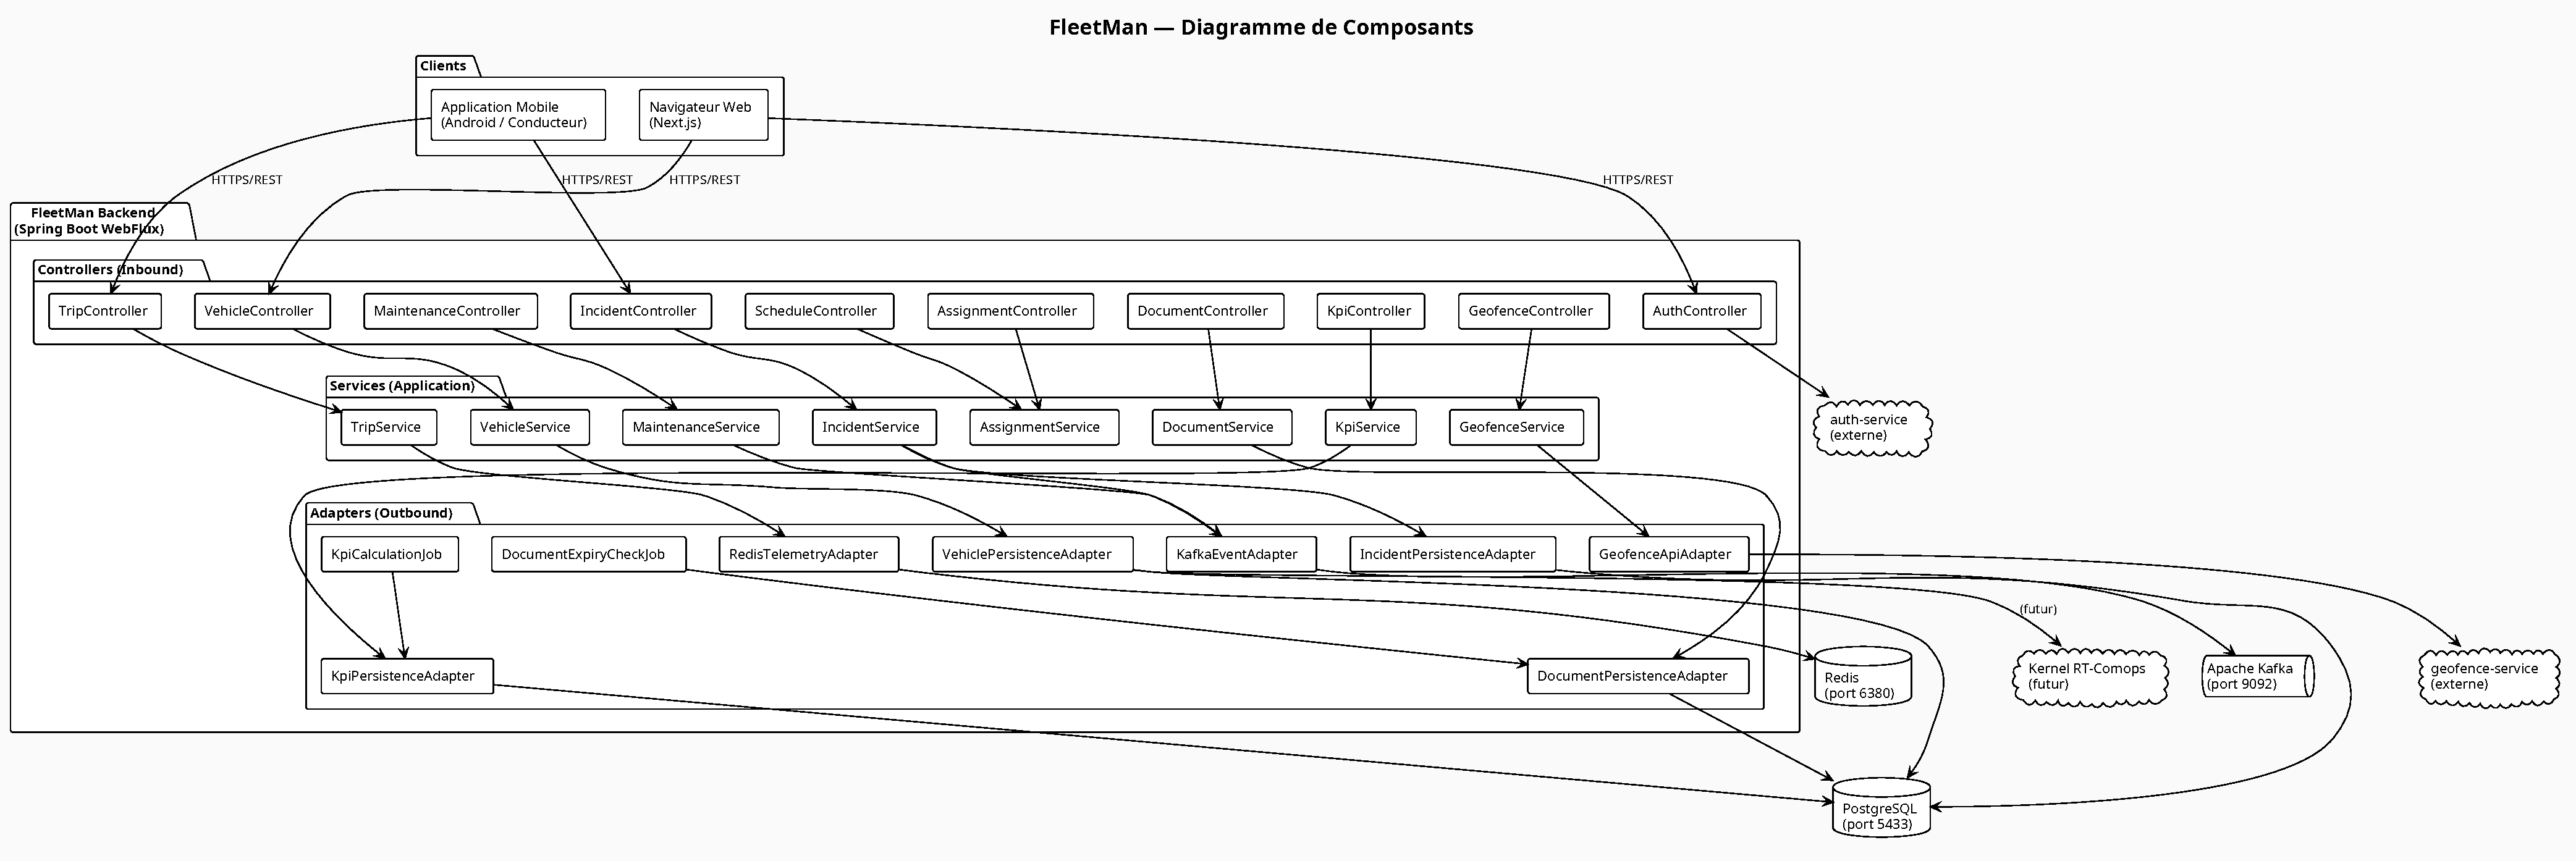
\includegraphics[height=0.90\textheight, keepaspectratio]{DiagrammeComposants}
  \caption{Diagramme de composants de FleetMan.
           Les composants internes (controllers, services, adapters) sont
           representes en bleu et vert~; les bases de donnees et services
           externes en gris et jaune. Les fleches pleines indiquent le sens
           des appels synchrones~; les fleches tiretees representent les
           flux asynchrones (Kafka, Redis pub/sub). Les composants sont
           regroupes par couche hexagonale~: infrastructure (inbound et
           outbound), application, et domaine.}
  \label{fig:composants}
\end{figure}
\end{landscape}

\begin{lecture}
Les controllers (inbound) recoivent les requetes HTTP et delegent
aux services. Les services orchestrent la logique metier et deleguent
la persistance aux adapters (outbound). Les jobs planifies s'executent
de facon autonome et utilisent les memes adapters que les services.
Le composant Redis est utilise pour deux usages distincts~: (1) cache
des positions GPS temps reel avec TTL de 5 minutes~; (2) cache des
permissions utilisateur pour eviter des appels repetitifs au service Auth.
Le composant Kafka sert de bus d'evenements asynchrone pour les notifications,
l'audit et l'integration avec d'autres modules RT-Comops.
\end{lecture}

\subsection{Patterns d'integration avec services externes}

FleetMan integre 4 services externes via des adapters dedies~:

\begin{table}[H]
\caption{Services externes et patterns d'integration}
\label{tab:external_services}
\centering\small
\begin{tabularx}{\textwidth}{p{3.5cm}p{2.5cm}X}
\toprule
\textbf{Service} & \textbf{Pattern} & \textbf{Usage} \\
\midrule
Auth Service      & Circuit Breaker & Validation JWT, recup claims utilisateur \\
Kernel Core       & Circuit Breaker + Cache & Consultation organisations, ressources \\
Maps/Geocoding    & Circuit Breaker + Fallback & Geocodage adresses, calcul itineraires \\
Notification Service & Fire-and-Forget (Kafka) & Envoi SMS/Email/Push aux conducteurs \\
\bottomrule
\end{tabularx}
\end{table}

Le Circuit Breaker Resilience4j est configure avec les seuils suivants~:
\begin{itemize}[leftmargin=2cm]
  \item \textbf{Failure rate threshold}~: 50\,\% (ouverture du circuit).
  \item \textbf{Wait duration in open state}~: 60 secondes.
  \item \textbf{Sliding window size}~: 10 requetes.
  \item \textbf{Fallback}~: Reponse degradee (ex~: adresse non geocodee).
\end{itemize}

\chapter{Modele de Donnees et Classes Metier}

\section{Diagramme de classes --- Couche domaine}

La figure~\ref{fig:classes_domaine} presente les entites metier
du domaine et leurs relations. Ces classes sont du Java pur,
sans aucune annotation Spring, JPA ou Jackson.

\subsection{Entites principales et leurs responsabilites}

\subsubsection{Entite Vehicle}

L'entite \texttt{Vehicle} est implementee comme un record Java immuable~:
\begin{verbatim}
public record Vehicle(
  UUID id,
  String licensePlate,
  String brand,
  String model,
  int year,
  VehicleType type,
  VehicleStatus status,
  UUID fleetId,
  String tenantId
) {
  // Validation dans le constructeur compact
}
\end{verbatim}

Les invariants valides sont~:
\begin{itemize}[leftmargin=2cm]
  \item \texttt{licensePlate} non vide et unique par tenant.
  \item \texttt{year} entre 1900 et annee courante + 1.
  \item \texttt{status} initialise a AVAILABLE par defaut.
\end{itemize}

\subsubsection{Entite Maintenance}

Contrairement a \texttt{Vehicle}, \texttt{Maintenance} est une classe
mutable car elle possede un cycle de vie avec changements d'etat~:

\begin{verbatim}
public class Maintenance {
  private UUID id;
  private UUID vehicleId;
  private MaintenanceType type;
  private MaintenanceStatus status;
  private LocalDateTime scheduledAt;
  private LocalDateTime completedAt;
  private BigDecimal cost;
  private String description;
  
  public void markAsCompleted(BigDecimal finalCost) {
    if (this.status != SCHEDULED) {
      throw new InvalidStateException();
    }
    this.status = COMPLETED;
    this.completedAt = LocalDateTime.now();
    this.cost = finalCost;
  }
}
\end{verbatim}

Les methodes metier (\texttt{markAsCompleted}, \texttt{cancel},
\texttt{reschedule}) encapsulent la logique de transition d'etat
et garantissent la coherence des donnees.

\subsubsection{Entite Incident}

L'entite \texttt{Incident} gere le cycle de vie complet d'un incident
terrain avec severite, resolution et impact operationnel~:

\begin{itemize}[leftmargin=2cm]
  \item \textbf{Severite}~: LOW, MEDIUM, HIGH, CRITICAL.
  \item \textbf{Statuts}~: OPEN, IN\_PROGRESS, RESOLVED, CLOSED.
  \item \textbf{Methodes metier}~: \texttt{resolve()}, \texttt{close()},
        \texttt{escalate()}, \texttt{isCritical()}.
\end{itemize}

Un incident CRITICAL bloque automatiquement le vehicule (statut MAINTENANCE)
et notifie le gestionnaire en temps reel via Kafka.

\subsubsection{Value Object Coordinates}

\texttt{Coordinates} est un Value Object immuable qui valide les bornes
GPS dans son constructeur~:

\begin{verbatim}
public record Coordinates(double latitude, double longitude) {
  public Coordinates {
    if (latitude < -90 || latitude > 90) {
      throw new InvalidCoordinatesException("Latitude invalide");
    }
    if (longitude < -180 || longitude > 180) {
      throw new InvalidCoordinatesException("Longitude invalide");
    }
  }
  
  public double distanceTo(Coordinates other) {
    // Formule de Haversine
  }
}
\end{verbatim}

Ce Value Object est utilise dans \texttt{TelemetryData}, \texttt{Geofence}
et \texttt{Trip}.

% PAGE DEDIEE EN PAYSAGE POUR LE DIAGRAMME DE CLASSES DOMAINE
\begin{landscape}
\begin{figure}[p]
  \centering
  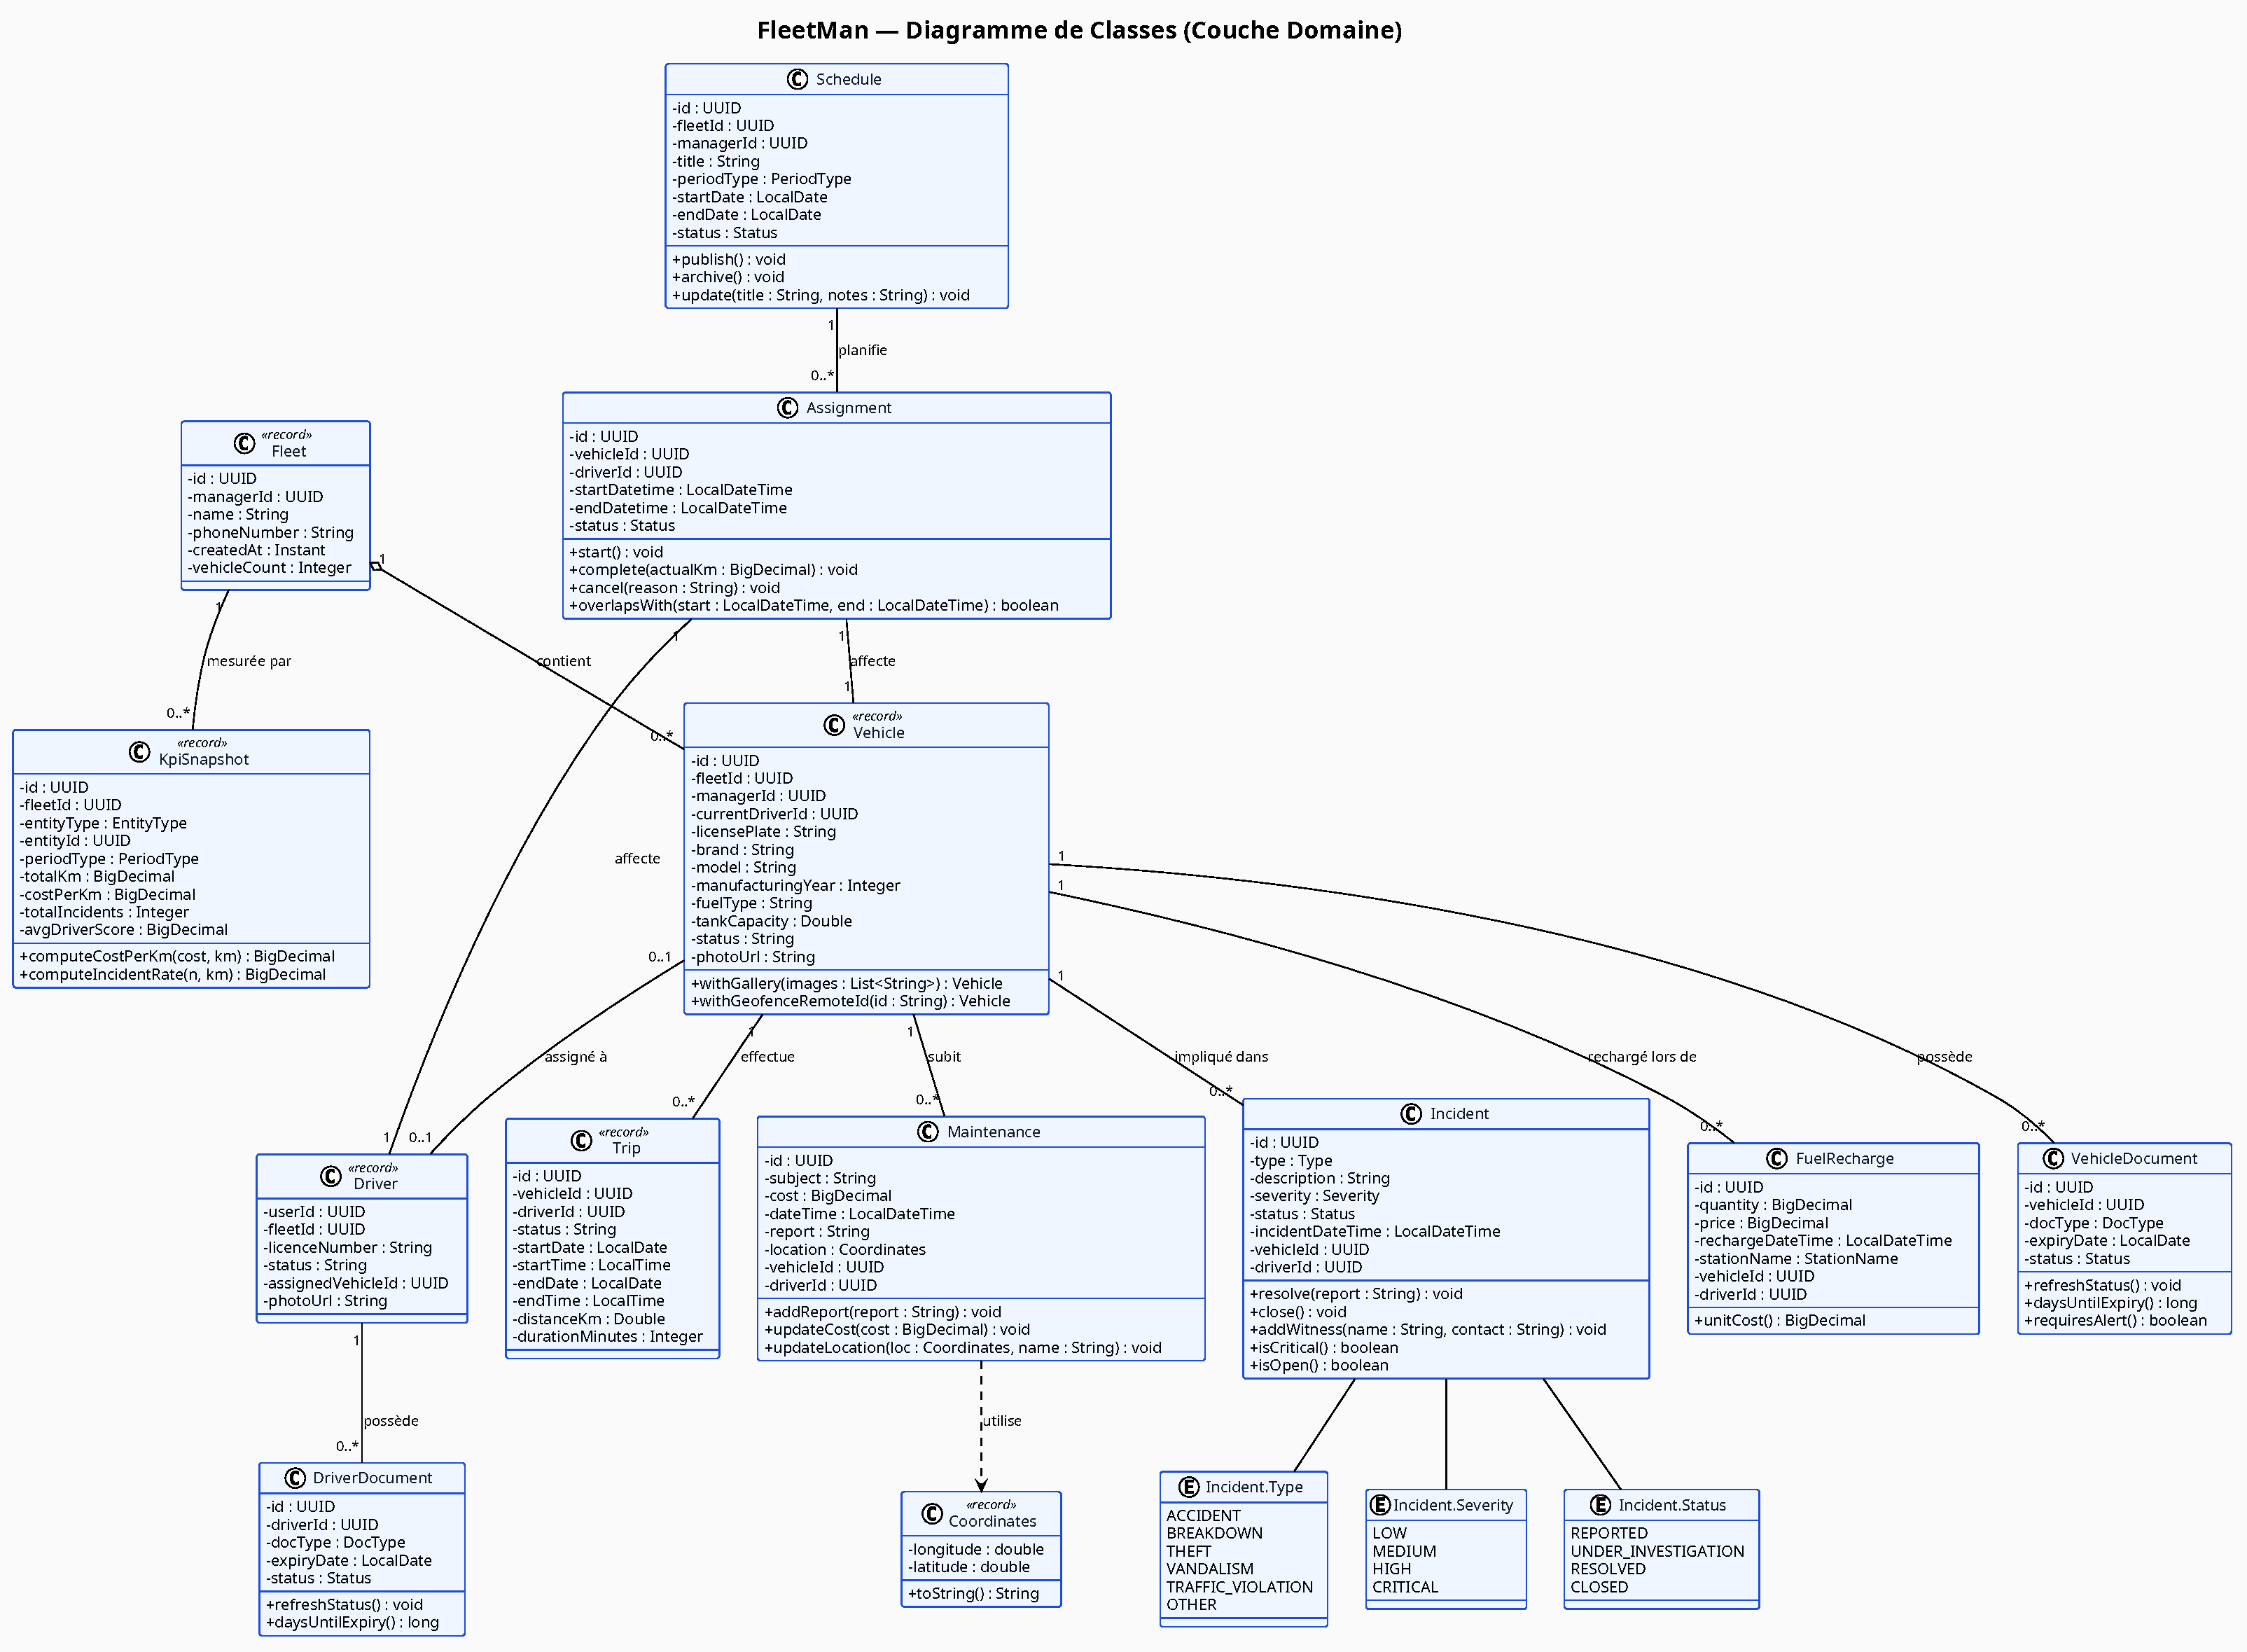
\includegraphics[height=0.90\textheight, keepaspectratio]{DiagrammeClasses_Domaine}
  \caption{Diagramme de classes de la couche domaine.
           Les records Java immuables (Vehicle, Fleet, Driver, Trip)
           sont distingues des classes avec etat mutable
           (Maintenance, Incident, Assignment). Les Value Objects
           (Coordinates, Address, Contact) sont representes avec le
           stereotype \guillemotleft{}ValueObject\guillemotright{}.
           Les enumerations (VehicleStatus, MaintenanceType, IncidentSeverity)
           definissent les etats autorises. Les relations de composition
           (losange noir) indiquent une dependance forte du cycle de vie~;
           les associations simples (fleches) representent des references
           par identifiant UUID.}
  \label{fig:classes_domaine}
\end{figure}
\end{landscape}

\begin{lecture}
Les entites \texttt{Maintenance}, \texttt{Incident} et \texttt{FuelRecharge}
sont des classes classiques car elles possedent des methodes metier qui
modifient leur etat (ex~: \texttt{resolve()}, \texttt{close()}).
Les entites \texttt{Vehicle}, \texttt{Fleet}, \texttt{Driver} et \texttt{Trip}
sont des records Java immuables car leur modification necessite une nouvelle
instance (immutabilite par conception).
L'entite \texttt{Coordinates} est un Value Object qui valide les bornes
GPS dans son constructeur. Les Value Objects sont systematiquement compares
par valeur (equals/hashCode sur tous les champs), pas par identite.
La relation entre \texttt{Vehicle} et \texttt{Fleet} est une association
simple (reference par UUID), permettant le changement de flotte sans
reconstruire le vehicule.
\end{lecture}

\subsection{Patterns DDD appliques}

Le modele de domaine applique 5 patterns du Domain-Driven Design~:

\begin{enumerate}[leftmargin=2cm]
  \item \textbf{Entity}~: Objets avec identite persistante (Vehicle, Driver,
        Trip, Maintenance, Incident). L'egalite se fait sur l'ID, pas sur
        les attributs.
        
  \item \textbf{Value Object}~: Objets sans identite, compares par valeur
        (Coordinates, Address, Contact, Money). Systematiquement immuables.
        
  \item \textbf{Aggregate Root}~: Entites racines qui controlent l'acces
        aux autres entites de l'agregat. Ex~: \texttt{Trip} est le root
        de l'agregat [Trip, TelemetryData[]]. Toute modification de
        telemetrie passe par Trip.
        
  \item \textbf{Factory Method}~: Methodes statiques de construction
        pour les entites complexes. Ex~: \texttt{Incident.critical()}
        pour creer un incident de severite CRITICAL.
        
  \item \textbf{Domain Event}~: Evenements metier publies apres operations
        critiques~: \texttt{VehicleCreated}, \texttt{TripStarted},
        \texttt{IncidentResolved}. Ces evenements sont publies sur Kafka
        pour l'integration asynchrone.
\end{enumerate}

\section{Diagramme de classes --- Ports et Adapters}

La figure~\ref{fig:classes_ports} illustre la structure des ports
et adapters, coeur du pattern hexagonal.

\subsection{Ports entrants (Inbound Ports / Use Cases)}

Les ports entrants definissent ce que le systeme offre a ses utilisateurs.
Chaque port correspond a un ensemble de use cases coherents~:

\begin{itemize}[leftmargin=2cm]
  \item \texttt{ManageVehicleUseCase}~: CRUD vehicules + historique + statistiques.
  \item \texttt{ManageDriverUseCase}~: CRUD conducteurs + evaluation + planning.
  \item \texttt{ManageTripUseCase}~: Creation, demarrage, cloture de trajets.
  \item \texttt{ManageIncidentUseCase}~: Declaration, suivi, resolution d'incidents.
  \item \texttt{ManageMaintenanceUseCase}~: Planification et suivi maintenances.
  \item \texttt{TrackVehicleUseCase}~: Reception telemetrie GPS, replay trajets.
  \item \texttt{ManageGeofenceUseCase}~: Definition zones, detection violations.
  \item \texttt{PlanScheduleUseCase}~: Creation plannings, gestion affectations.
  \item \texttt{ComputeKpiUseCase}~: Calcul et consultation indicateurs.
\end{itemize}

Chaque use case est une interface Java pure, sans dependance Spring~:

\begin{verbatim}
public interface ManageVehicleUseCase {
  Mono<Vehicle> create(CreateVehicleCommand cmd);
  Mono<Vehicle> findById(UUID id);
  Flux<Vehicle> findAll(Pageable pageable);
  Mono<Vehicle> update(UUID id, UpdateVehicleCommand cmd);
  Mono<Void> archive(UUID id);
}
\end{verbatim}

\subsection{Ports sortants (Outbound Ports)}

Les ports sortants definissent ce que le domaine requiert de l'infrastructure.
Ils sont implementes par des adapters dans la couche infrastructure~:

\begin{itemize}[leftmargin=2cm]
  \item \textbf{PersistencePorts}~: \texttt{VehiclePersistencePort},
        \texttt{DriverPersistencePort}, \texttt{TripPersistencePort}, etc.
        Chaque port expose des methodes reactives (Mono, Flux) pour
        les operations CRUD.
        
  \item \textbf{MessagingPorts}~: \texttt{OperationEventPort},
        \texttt{TelemetryEventPort}. Publication asynchrone d'evenements
        metier sur Kafka.
        
  \item \textbf{CachePorts}~: \texttt{TelemetryCachePort},
        \texttt{PermissionCachePort}. Acces temps reel aux donnees
        cached dans Redis.
        
  \item \textbf{ExternalServicePorts}~: \texttt{AuthServicePort},
        \texttt{KernelServicePort}, \texttt{GeocodingServicePort}.
        Appels HTTP vers services externes avec Circuit Breaker.
\end{itemize}

% PAGE DEDIEE EN PAYSAGE POUR LE DIAGRAMME DE CLASSES PORTS
\begin{landscape}
\begin{figure}[p]
  \centering
  
\includegraphics[height=0.90\textheight, keepaspectratio]{DiagrammeClasses_Ports}
  \caption{Diagramme de classes des Ports et Adapters.
           Les interfaces de ports entrants (use cases) sont representees
           en vert a gauche~; les interfaces de ports sortants en orange
           a droite. Les implementations de use cases (services) sont en
           bleu au centre. Les adapters d'infrastructure (en gris) implementent
           les ports sortants. Les fleches en tirets symbolisent les relations
           d'implementation (\guillemotleft{}implements\guillemotright{}).
           Les fleches pleines representent les relations d'utilisation
           (\guillemotleft{}uses\guillemotright{}). Cette organisation garantit
           que le domaine ne depend d'aucune technologie concrete (inversion
           de dependance).}
  \label{fig:classes_ports}
\end{figure}
\end{landscape}

\begin{lecture}
Les interfaces \texttt{ManageVehicleUseCase}, \texttt{ManageIncidentUseCase}, etc.
constituent les ports entrants~: ce que le domaine offre.
Les interfaces \texttt{VehiclePersistencePort}, \texttt{OperationEventPort}, etc.
constituent les ports sortants~: ce que le domaine requiert.
Les adapters d'infrastructure implementent les ports sortants sans que
le domaine ne les connaisse directement. Cette separation permet de remplacer
PostgreSQL par MongoDB ou Kafka par RabbitMQ sans modifier une seule ligne
du domaine. Les services (implementations des use cases) orchestrent les
ports sortants pour realiser la logique metier.
\end{lecture}

\subsection{Avantages du pattern Ports \& Adapters}

\begin{enumerate}[leftmargin=2cm]
  \item \textbf{Testabilite}~: Les use cases peuvent etre testes unitairement
        en mockant les ports sortants (pas besoin de base de donnees reelle).
        
  \item \textbf{Independance technologique}~: Le domaine ne connait ni Spring,
        ni R2DBC, ni Kafka. Il peut etre extrait vers un autre framework
        sans refactorisation.
        
  \item \textbf{Evolutivite}~: Ajouter un nouveau canal d'entree (GraphQL,
        gRPC) necessite uniquement un nouvel adapter inbound appelant
        les use cases existants.
        
  \item \textbf{Maintenabilite}~: La logique metier est centralisee dans
        les services, pas eparpillee dans les controllers ou repositories.
        
  \item \textbf{Migration microservices}~: Chaque bounded context (vehicules,
        conducteurs, trajets) peut etre extrait en microservice independant
        en packagant son domaine + ses adapters.
\end{enumerate}

\section{Diagramme de deploiement}

La figure~\ref{fig:deploiement} decrit l'architecture de deploiement
en environnement local via Docker Compose.

\subsection{Environnements de deploiement}

FleetMan supporte 4 environnements avec configurations distinctes~:

\begin{enumerate}[leftmargin=2cm]
  \item \textbf{Local (dev)}~: Application Spring Boot lancee depuis l'IDE,
        services externes (PostgreSQL, Redis, Kafka) en conteneurs Docker.
        Hot-reload active via Spring DevTools.
        
  \item \textbf{Integration (int)}~: Tous les composants dockerises,
        deployes via Docker Compose sur machine de CI/CD. Utilise pour
        les tests d'integration et end-to-end.
        
  \item \textbf{Staging (staging)}~: Infrastructure Kubernetes (AWS EKS),
        bases de donnees managees (RDS PostgreSQL, ElastiCache Redis),
        Kafka MSK. Replication de la production a echelle reduite.
        
  \item \textbf{Production (prod)}~: Infrastructure Kubernetes avec
        auto-scaling (HPA), multi-AZ pour haute disponibilite, monitoring
        Prometheus/Grafana, logs centralises ElasticSearch/Kibana.
\end{enumerate}

\subsection{Configuration Docker Compose locale}

Le fichier \texttt{docker-compose.yml} definit 3 services~:

\begin{verbatim}
version: '3.9'
services:
  postgres:
    image: postgis/postgis:16-alpine
    ports: ["5433:5432"]
    environment:
      POSTGRES_DB: fleetman
      POSTGRES_USER: fleet_user
      POSTGRES_PASSWORD: fleet_pass
    volumes:
      - postgres_data:/var/lib/postgresql/data
      
  redis:
    image: redis:7-alpine
    ports: ["6380:6379"]
    command: redis-server --maxmemory 512mb --maxmemory-policy allkeys-lru
    
  kafka:
    image: apache/kafka:3.7.0
    ports: ["9092:9092"]
    environment:
      KAFKA_PROCESS_ROLES: broker,controller
      KAFKA_NODE_ID: 1
      # Mode KRaft (sans ZooKeeper)
\end{verbatim}

\subsection{Specifications techniques minimales}

\begin{table}[H]
\caption{Specifications techniques par environnement}
\label{tab:specs_deploy}
\centering\small
\begin{tabularx}{\textwidth}{p{2.5cm}p{2cm}p{2cm}p{2cm}X}
\toprule
\textbf{Ressource} & \textbf{Local} & \textbf{Int} & \textbf{Staging} & \textbf{Production} \\
\midrule
CPU (cores)         & 2    & 4    & 8     & 16 (auto-scale) \\
RAM (GB)            & 4    & 8    & 16    & 32 (auto-scale) \\
Disk (GB)           & 20   & 50   & 200   & 500 (SSD) \\
PostgreSQL (vCPU)   & 2    & 2    & 4     & 8 (RDS Multi-AZ) \\
Redis (GB)          & 0.5  & 1    & 2     & 4 (ElastiCache) \\
Kafka (partitions)  & 3    & 6    & 12    & 24 (MSK) \\
Replicas (pods)     & 1    & 2    & 3     & 5 min, 20 max \\
\bottomrule
\end{tabularx}
\end{table}

% PAGE DEDIEE EN PAYSAGE POUR LE DIAGRAMME DE DEPLOIEMENT
\begin{landscape}
\begin{figure}[p]
  \centering
  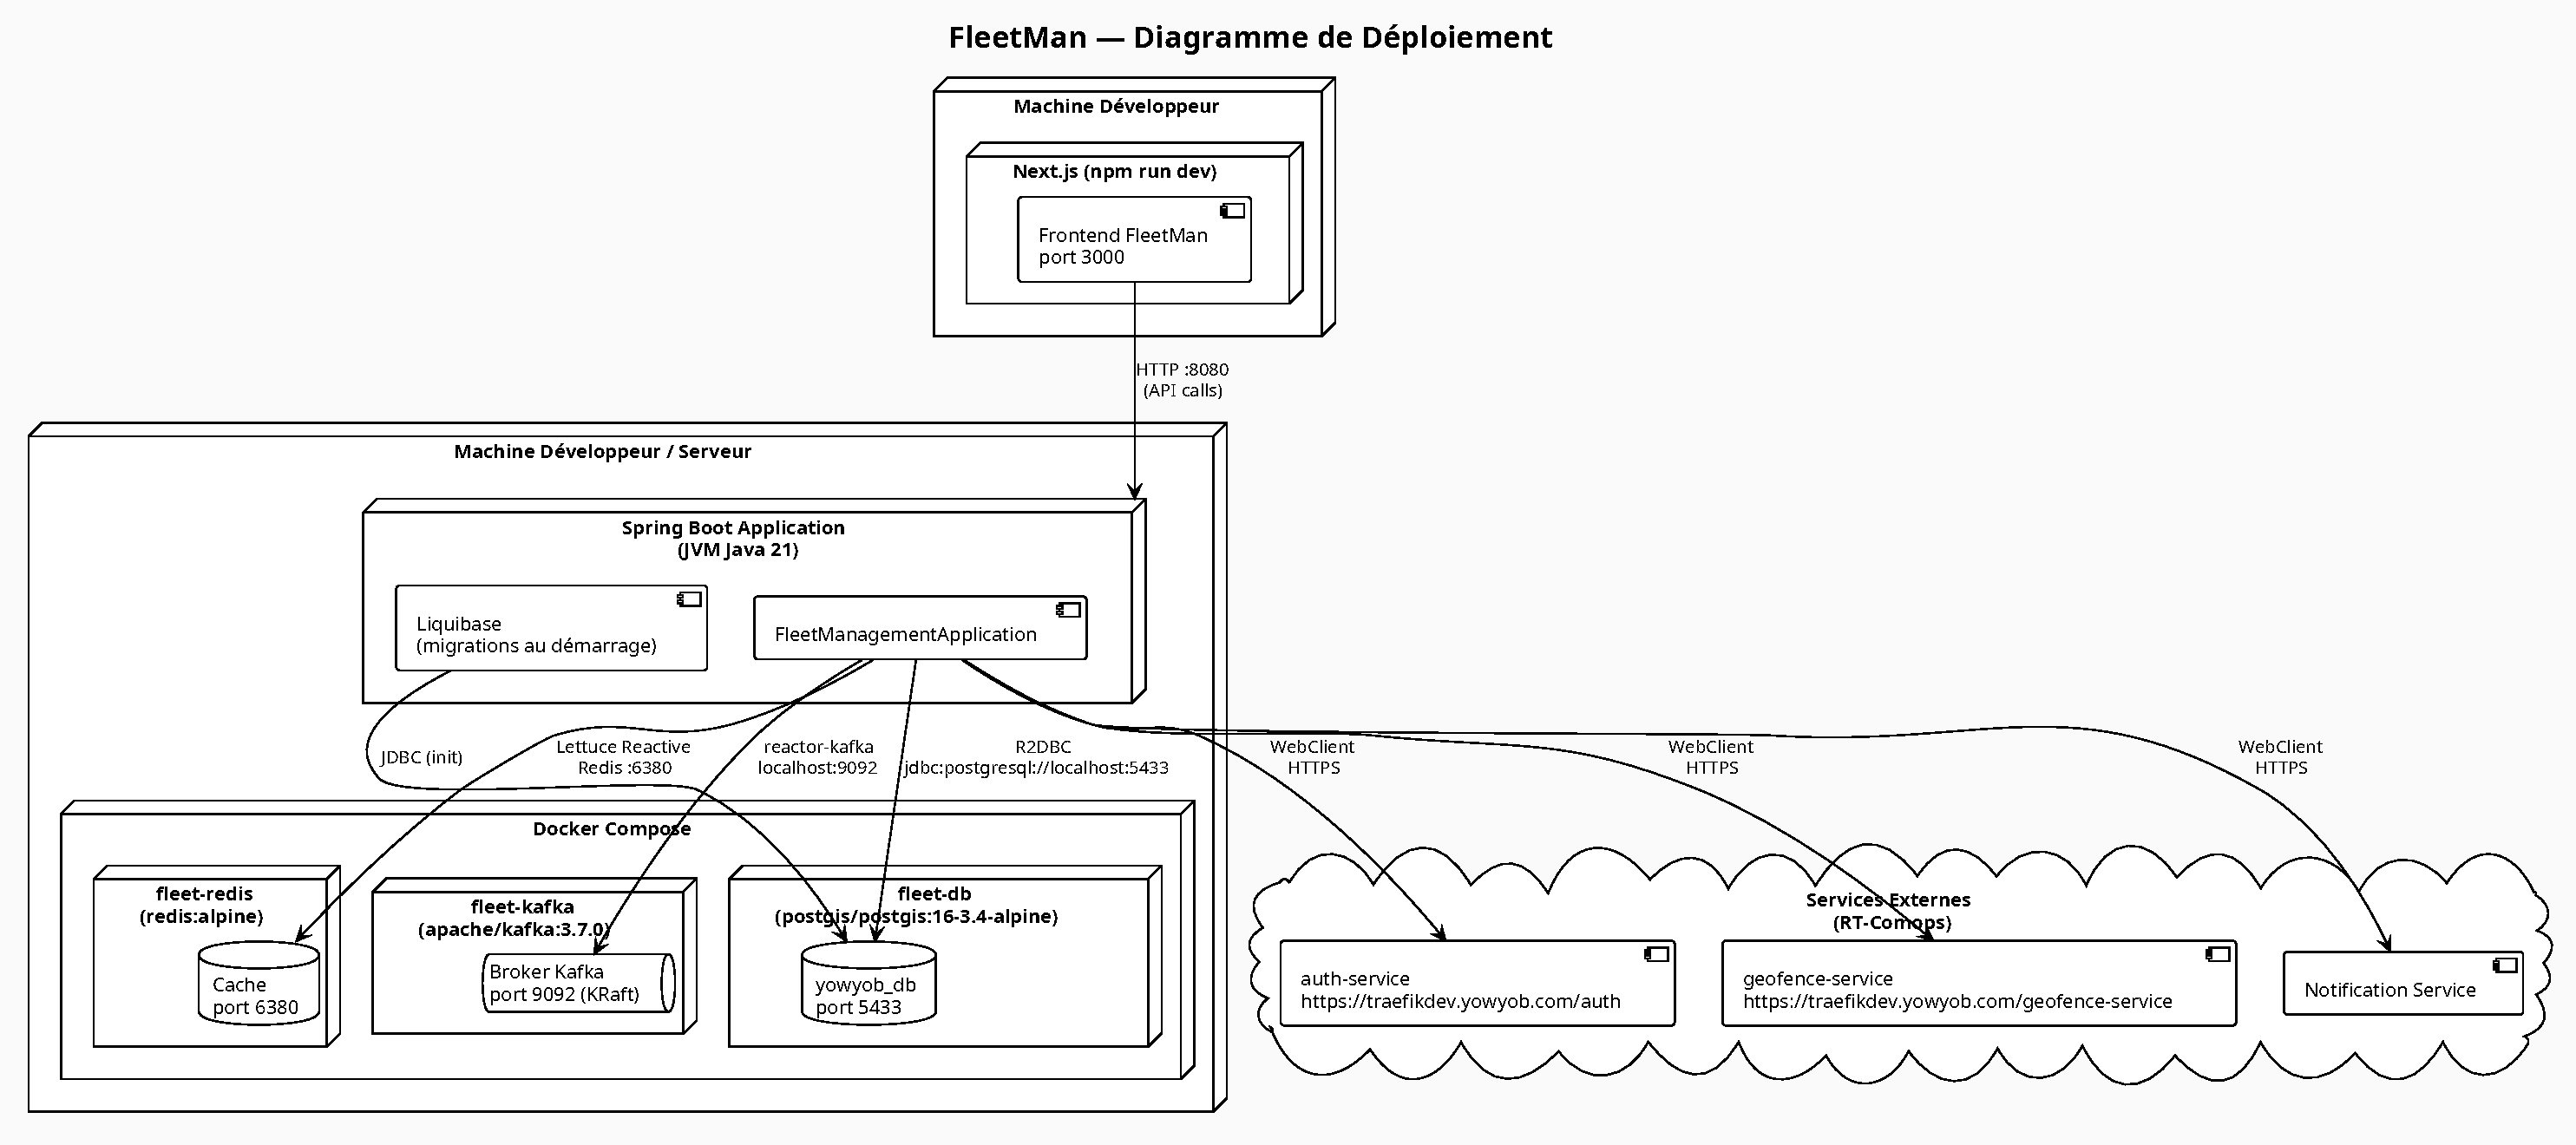
\includegraphics[height=0.90\textheight, keepaspectratio]{DiagrammeDeploiement}
  \caption{Diagramme de deploiement de FleetMan en environnement local.
           Trois conteneurs Docker~: PostgreSQL avec extension PostGIS
           (port 5433), Redis avec politique LRU (port 6380) et Kafka
           en mode KRaft sans ZooKeeper (port 9092).
           L'application Spring Boot communique avec PostgreSQL via R2DBC
           (driver reactif), avec Redis via Lettuce (client reactif) et
           avec Kafka via Spring Cloud Stream. Les services externes
           (Auth, Kernel, Maps) sont accedes via HTTPS avec Circuit Breaker
           Resilience4j. Liquibase s'execute au demarrage de l'application
           pour appliquer les 10 migrations de schema de facon incrementale.}
  \label{fig:deploiement}
\end{figure}
\end{landscape}

\begin{lecture}
Les boites representent les noeuds de deploiement.
L'application Spring Boot est lancee directement sur la JVM Java 21
(hors Docker en developpement). Liquibase s'execute au demarrage
de l'application pour appliquer les migrations de schema de maniere
incrementale et idempotente. Les conteneurs Docker sont orchestres
via docker-compose.yml pour faciliter la reproductibilite de l'environnement
de developpement. En production, l'application est packagee en image Docker
multi-stage (build + runtime) et deployee sur Kubernetes avec Helm charts.
Le health check endpoint \texttt{/actuator/health} est utilise par
Kubernetes pour les liveness et readiness probes.
\end{lecture}

\subsection{Strategie de deploiement en production}

Le deploiement en production suit une strategie Blue-Green avec validation
automatisee~:

\begin{enumerate}[leftmargin=2cm]
  \item \textbf{Build}~: Compilation Maven, tests unitaires + integration,
        analyse SonarQube, scan vulnerabilites (Trivy).
        
  \item \textbf{Package}~: Construction image Docker multi-stage,
        push vers AWS ECR avec tag semantique (semver).
        
  \item \textbf{Deploy Green}~: Deploiement version N+1 sur environnement
        Green (parallele au Blue), sans trafic reel.
        
  \item \textbf{Smoke Tests}~: Execution tests sante (health checks,
        endpoints critiques, conectivite bases de donnees).
        
  \item \textbf{Switch}~: Bascule trafic du Blue vers Green via load
        balancer AWS ALB avec strategie weighted (10\% -> 50\% -> 100\%).
        
  \item \textbf{Monitor}~: Surveillance metriques (latence P95, taux erreur,
        CPU/RAM) pendant 15 minutes.
        
  \item \textbf{Rollback automatique}~: Si taux erreur > 1\%, rollback
        instantane vers version Blue precedente.
\end{enumerate}

Cette strategie garantit un deploiement zero-downtime et un rollback
rapide en cas de regression.

% =============================================================================
\part{Conception des Modules Metier}
% =============================================================================

\chapter{Modules du Coeur Metier Initial}

\section{Module Authentification --- Diagramme de sequence}

La figure~\ref{fig:seq_auth} detaille le flux complet d'authentification
d'un utilisateur, depuis la soumission des identifiants jusqu'a
l'injection du contexte de securite dans la chaine reactive.

\subsection{Flux d'authentification détaillé}

Le processus d'authentification FleetMan suit un flux \textbf{Kernel en deux
étapes}, implémenté dans \texttt{KernelAuthAdapter}~:

\begin{enumerate}[leftmargin=2cm]
  \item \textbf{Discover contexts}~: \texttt{POST /api/auth/discover-contexts}
        avec \texttt{principal} et \texttt{password}. Le Kernel retourne un
        \texttt{selectionToken} et la liste des contextes accessibles
        (admin, gestionnaire, conducteur).
  \item \textbf{Select context}~: \texttt{POST /api/auth/select-context} avec
        le \texttt{selectionToken}, le \texttt{contextId} choisi et
        éventuellement \texttt{organizationId} (null pour gestionnaires
        et conducteurs dont la liste d'organisations est vide).
  \item \textbf{JWT RS256}~: le Kernel émet \texttt{accessToken} et
        \texttt{refreshToken}. Les rôles sont extraits du claim
        \texttt{permissions} (source fiable, car \texttt{/api/users/me}
        ne retourne pas toujours les authorities).
  \item \textbf{Rebind UUID local}~: \texttt{JwtAuthenticationManager} associe
        le \texttt{sub} Kernel au \texttt{users.kernel\_id} PostgreSQL pour
        la traçabilité locale.
\end{enumerate}

Le profil \texttt{fake-auth} (\texttt{FakeAuthAdapter}) reste disponible pour
le développement local sans accès Kernel. Le frontend rejette automatiquement
les anciens tokens \texttt{fake-token-*} stockés en session.

\subsection{Securite du token JWT}

Le token JWT utilise l'algorithme RS256 (RSA + SHA-256) avec les caracteristiques
suivantes~:

\begin{itemize}[leftmargin=2cm]
  \item \textbf{Cle privee}~: 2048 bits, stockee dans AWS Secrets Manager,
        rotee tous les 90 jours.
  \item \textbf{Cle publique}~: Distribuee aux services via endpoint JWK
        (\texttt{/.well-known/jwks.json}).
  \item \textbf{Claims standards}~: \texttt{iss} (issuer), \texttt{sub}
        (subject=userId), \texttt{iat} (issued at), \texttt{exp}
        (expiration=24h).
  \item \textbf{Claims customs}~: \texttt{tenantId}, \texttt{roles[]},
        \texttt{permissions[]}, \texttt{fleetIds[]}.
\end{itemize}

\subsection{Gestion des sessions et revocation}

FleetMan maintient une table \texttt{user\_sessions} pour tracer les
sessions actives~:

\begin{verbatim}
CREATE TABLE user_sessions (
  id UUID PRIMARY KEY,
  user_id UUID NOT NULL,
  token_jti VARCHAR(36) NOT NULL UNIQUE,
  created_at TIMESTAMP NOT NULL,
  expires_at TIMESTAMP NOT NULL,
  last_activity TIMESTAMP,
  ip_address INET,
  user_agent TEXT,
  revoked BOOLEAN DEFAULT false
);
\end{verbatim}

La revocation d'une session specifique marque \texttt{revoked=true} et
ajoute le \texttt{token\_jti} dans une blacklist Redis (TTL = duree residuelle
du token). Toutes les requetes verifient la blacklist avant d'autoriser l'acces.

% PAGE DEDIEE EN PAYSAGE POUR LE DIAGRAMME DE SEQUENCE AUTH
\begin{landscape}
\begin{figure}[p]
  \centering
  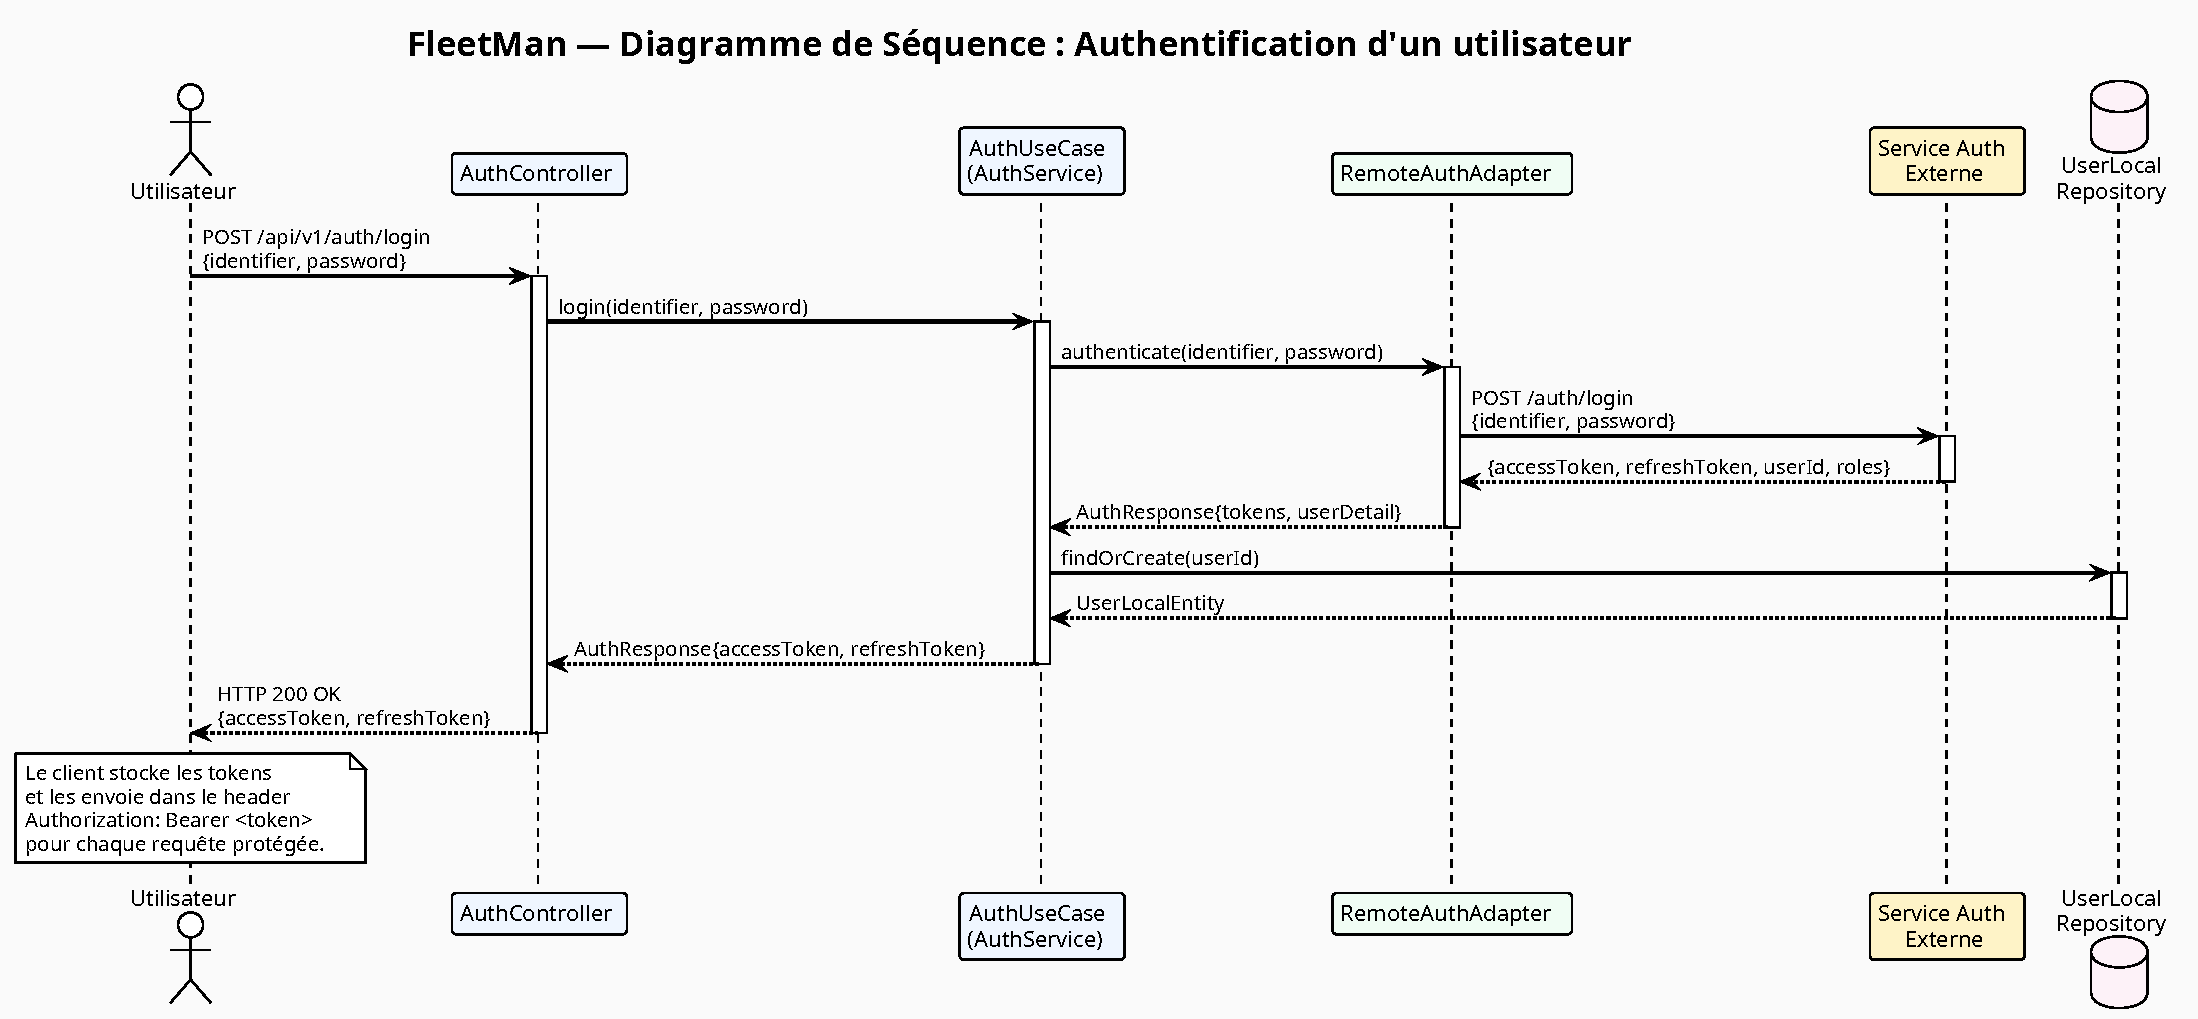
\includegraphics[height=0.90\textheight, keepaspectratio]{DiagrammeSequence_Auth}
  \caption{Diagramme de sequence~: Authentification d'un utilisateur.
           La fleche (1) initie l'appel HTTP POST \texttt{/api/v1/auth/login}
           avec email et password~; les fleches (2)--(3) illustrent
           la delegation au service Auth externe via WebClient reactif~;
           la fleche (4) montre le rapatriement du token JWT RS256~;
           les fleches (5)--(6) representent la creation/mise a jour
           de l'utilisateur local et le cache des permissions dans Redis~;
           la fleche (7) retourne le token au client.
           Le diagramme inclut egalement le flux de validation de token
           pour les requetes subsequentes (partie droite)~: extraction
           du token depuis l'en-tete Authorization, validation de la
           signature RS256, verification de l'expiration, consultation
           de la blacklist Redis, et injection du contexte de securite.}
  \label{fig:seq_auth}
\end{figure}
\end{landscape}

\begin{lecture}
Le diagramme de la figure~\ref{fig:seq_auth} a été mis à jour pour refléter
le flux Kernel en deux étapes (\texttt{discover-contexts} puis
\texttt{select-context}). L'ancien schéma d'authentification locale directe
est obsolète. Le code PlantUML de régénération est fourni dans
\texttt{diagrammes\_plantuml.md}.
\end{lecture}

\subsection{Mecanisme de rafraichissement de token}

FleetMan implemente un mecanisme de refresh token pour les sessions longues~:

\begin{itemize}[leftmargin=2cm]
  \item \textbf{Access token}~: Duree de vie courte (15 minutes), contient
        toutes les permissions, utilise pour chaque requete API.
        
  \item \textbf{Refresh token}~: Duree de vie longue (7 jours), stocke
        en HTTP-only cookie secure, utilise uniquement pour obtenir un
        nouvel access token.
        
  \item \textbf{Rotation}~: A chaque utilisation du refresh token, un nouveau
        refresh token est genere et l'ancien est revoque (rotation pour
        limiter le risque de vol).
\end{itemize}

Cette strategie equilibre securite (access token court limite l'exposition
en cas de vol) et experience utilisateur (pas de re-login toutes les
15 minutes).

\section{Module Vehicule --- Machine a etats}

\begin{figure}[H]
  \centering
  \begin{tikzpicture}[
    state/.style={rectangle, rounded corners=8pt, minimum width=3cm,
                  minimum height=0.8cm, draw=fleetblue, fill=fleetblue!10,
                  font=\small\bfseries},
    arrow/.style={->, >=Stealth, thick}
  ]
    \node[state]                                     (av) at (0,0)     {AVAILABLE};
    \node[state, draw=fleetwarning, fill=fleetwarning!10] (ot) at (5,0)  {ON\_TRIP};
    \node[state, draw=fleeterror,   fill=fleeterror!10]   (ma) at (2.5,-2.5) {MAINTENANCE};
    \draw[arrow] (av) to[bend left=15]  node[above,font=\small] {startTrip()} (ot);
    \draw[arrow] (ot) to[bend left=15]  node[below,font=\small] {endTrip()}   (av);
    \draw[arrow] (av) -- node[left, font=\small] {sendToMaint()} (ma);
    \draw[arrow] (ma) -- node[right,font=\small] {returnFromMaint()} (av);
  \end{tikzpicture}
  \caption{Machine a etats du vehicule FleetMan.
           Le statut AVAILABLE est l'etat initial.
           Seul un vehicule AVAILABLE peut demarrer un trajet.
           Un vehicule en MAINTENANCE ne peut pas etre affecte.}
  \label{fig:vehicle_states}
\end{figure}

\section{Module Trajet --- Diagramme d'etats}

La figure~\ref{fig:states_trip} presente le cycle de vie complet
d'un trajet depuis sa creation jusqu'a sa cloture.

\subsection{Etats du trajet et transitions}

Le cycle de vie d'un trajet comprend 5 etats principaux~:

\begin{enumerate}[leftmargin=2cm]
  \item \textbf{PLANNED}~: Etat initial apres creation. Le trajet est
        planifie mais pas encore demarre. Le gestionnaire peut modifier
        les details (depart, arrivee, conducteur, vehicule).
        
  \item \textbf{READY}~: Le conducteur a valide sa disponibilite et le
        vehicule est pret (statut AVAILABLE, niveau carburant suffisant,
        aucun document expire). Transition automatique depuis PLANNED
        ou declenchee manuellement.
        
  \item \textbf{ONGOING}~: Trajet en cours d'execution. Le conducteur envoie
        la telemetrie GPS toutes les 30 secondes. Le georeperage est actif.
        Les evenements de conduite (exces de vitesse, freinages brusques)
        sont detectes en temps reel.
        
  \item \textbf{COMPLETED}~: Trajet termine avec succes. La distance reelle,
        la duree et la consommation carburant sont automatiquement calculees.
        Le score de conduite du conducteur est mis a jour.
        
  \item \textbf{CANCELLED}~: Trajet annule avant ou pendant l'execution.
        Necessite un motif obligatoire (panne vehicule, indisponibilite
        conducteur, mission annulee par le client).
\end{enumerate}

\subsection{Regles metier des transitions}

Chaque transition est soumise a des preconditions strictes~:

\begin{itemize}[leftmargin=2cm]
  \item \textbf{PLANNED $\to$ READY}~: Vehicule AVAILABLE, conducteur ACTIVE,
        pas de conflit d'affectation, documents vehicule et conducteur valides.
        
  \item \textbf{READY $\to$ ONGOING}~: Declenchee uniquement par le conducteur
        via l'application mobile ou le dashboard. Horodatage GPS initial obligatoire.
        
  \item \textbf{ONGOING $\to$ COMPLETED}~: Distance minimale de 1 km parcourue,
        duree minimale de 5 minutes. Horodatage GPS final obligatoire.
        
  \item \textbf{* $\to$ CANCELLED}~: Possible depuis PLANNED, READY ou ONGOING.
        Depuis ONGOING, necessite validation du gestionnaire (annulation tardive).
\end{itemize}

\subsection{Calculs automatises lors de la completion}

Au passage en etat COMPLETED, plusieurs calculs sont executes automatiquement~:

\begin{enumerate}[leftmargin=2cm]
  \item \textbf{Distance reelle}~: Sommation des distances entre points GPS
        consecutifs (formule de Haversine).
        
  \item \textbf{Duree reelle}~: Difference entre \texttt{endedAt} et
        \texttt{startedAt}, decomposee en heures effectives (hors pauses).
        
  \item \textbf{Consommation estimee}~: Calcul base sur la consommation
        moyenne du vehicule (L/100km) et la distance reelle.
        
  \item \textbf{Cout estime}~: Distance $\times$ cout kilom\'etrique
        (carburant + amortissement + maintenance repartie).
        
  \item \textbf{Score de conduite}~: Agregation des evenements detectes
        (exces vitesse, freinages brusques, accelerations, virages serres)
        via l'algorithme de scoring (voir algorithme~\ref{alg:scoring}).
        
  \item \textbf{Ecarts par rapport au plan}~: Comparaison distance
        reelle vs estimee, duree reelle vs estimee, avec calcul des taux
        d'ecart en pourcentage.
\end{enumerate}

% PAGE DEDIEE POUR LE DIAGRAMME D'ETATS TRIP
\begin{figure}[p]
  \centering
  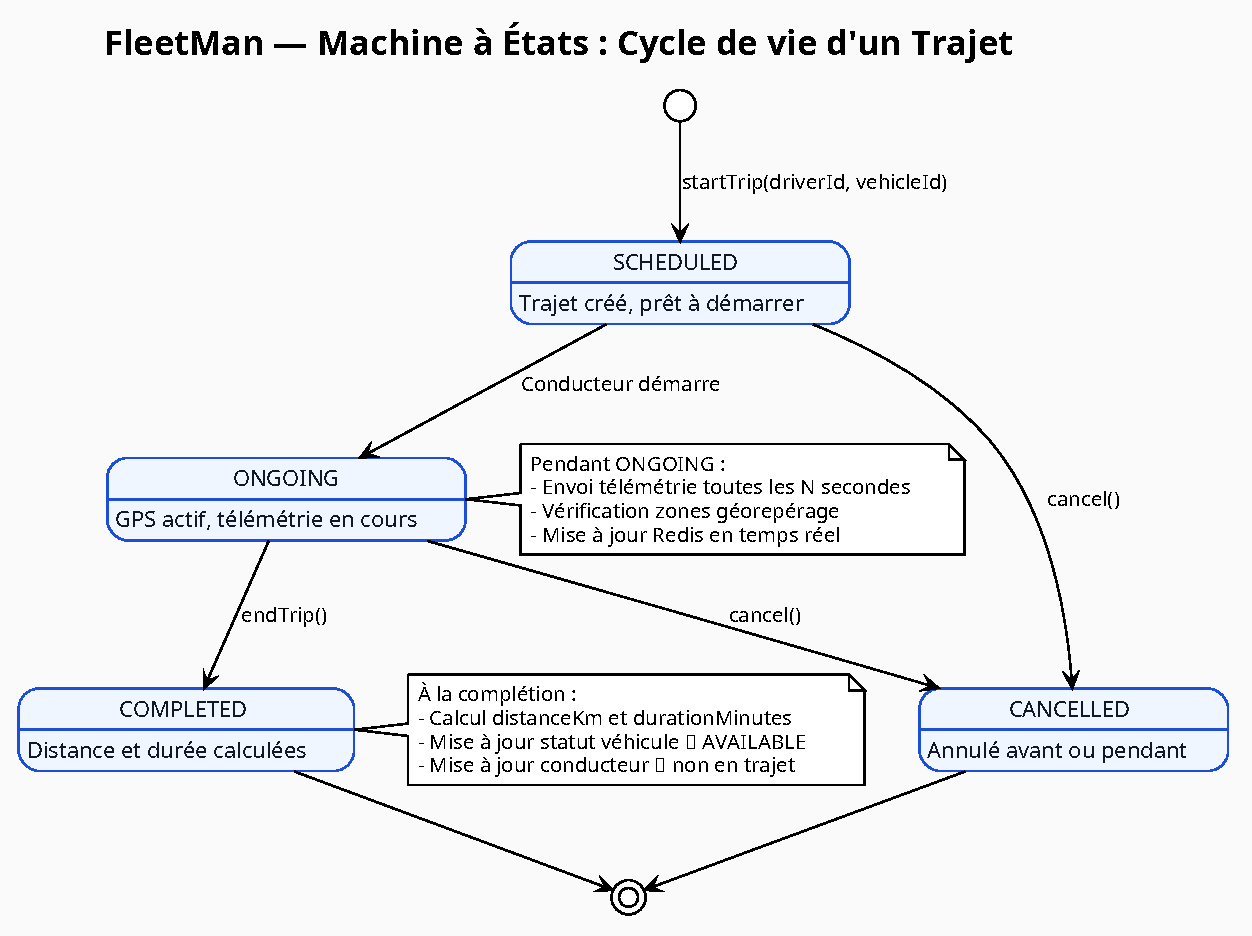
\includegraphics[width=0.95\textwidth, keepaspectratio]{DiagrammeEtats_Trip}
  \caption{Diagramme d'etats~: Cycle de vie d'un Trajet.
           Les transitions sont declenchees par les actions du conducteur
           (\texttt{startTrip}, \texttt{endTrip}) ou du gestionnaire
           (\texttt{cancel}). Les etats PLANNED et READY sont des etats
           preparatoires sans telemetrie GPS. L'etat ONGOING est l'etat
           actif durant lequel le conducteur envoie des donnees de telemetrie
           toutes les 30 secondes et le georeperage est active. L'etat
           COMPLETED est terminal et declenche les calculs automatises
           (distance, duree, consommation, score de conduite). L'etat
           CANCELLED peut etre atteint depuis n'importe quel etat non
           terminal et necessite un motif obligatoire.}
  \label{fig:states_trip}
\end{figure}

\begin{lecture}
L'etat \texttt{ONGOING} est l'etat actif durant lequel le conducteur
envoie des donnees de telemetrie GPS toutes les 30 secondes. C'est dans
cet etat que le georeperage est actif et que les evenements de conduite
sont detectes en temps reel. L'etat \texttt{COMPLETED} calcule automatiquement
la distance parcourue (sommation des segments GPS via formule de Haversine),
la duree du trajet (difference timestamps debut/fin), la consommation carburant
estimee (distance $\times$ conso moyenne vehicule), et le score de conduite
du conducteur (penalites basees sur les evenements detectes). Ces calculs
sont executes de facon asynchrone dans un job reactif pour ne pas bloquer
la reponse HTTP au conducteur. L'etat \texttt{CANCELLED} preserve toutes
les donnees collectees jusqu'au point d'annulation pour analyse ulterieure
(telemetrie partielle, evenements detectes, carburant consomme).
\end{lecture}

\subsection{Persistance de la telemetrie GPS}

La telemetrie GPS suit une strategie de stockage hybride~:

\begin{itemize}[leftmargin=2cm]
  \item \textbf{Redis (temps reel)}~: Derniere position de chaque vehicule
        active, avec TTL de 5 minutes. Utilisee pour l'affichage carte
        temps reel sur le dashboard.
        
  \item \textbf{Kafka (streaming)}~: Tous les points GPS publies sur topic
        \texttt{fleetman.telemetry.gps} pour consommation par services
        externes (georeperage, analytics, replay).
        
  \item \textbf{PostgreSQL (historique)}~: Points GPS decimes (1 point toutes
        les 2 minutes) stockes dans la table \texttt{trip\_telemetry}
        pour les replays et analyses historiques. Partition mensuelle
        pour optimiser les requetes.
\end{itemize}

Cette architecture garantit des performances optimales pour l'affichage
temps reel (Redis) tout en preservant l'historique complet (Kafka + PostgreSQL).

\section{Module Georeperage --- Diagramme de sequence}

La figure~\ref{fig:seq_gps} illustre le flux de telemetrie GPS
et le declenchement automatique des alertes de georeperage.

\subsection{Architecture du module de georeperage}

Le georeperage FleetMan s'appuie sur l'extension PostGIS de PostgreSQL
pour les calculs geometriques~:

\begin{enumerate}[leftmargin=2cm]
  \item \textbf{Definition des zones}~: Le gestionnaire trace des polygones
        sur une carte interactive (React Leaflet). Les coordonnees sont
        envoyees au backend et persistees en format GeoJSON dans la colonne
        \texttt{boundary GEOMETRY(POLYGON, 4326)}.
        
  \item \textbf{Types de zones}~: INCLUSION (le vehicule doit rester a
        l'interieur), EXCLUSION (le vehicule ne doit pas entrer), CHECKPOINT
        (le vehicule doit passer par la zone).
        
  \item \textbf{Detection en temps reel}~: A chaque reception de telemetrie
        GPS, une requete PostGIS verifie si le point est dans/hors des zones
        actives via la fonction \texttt{ST\_Contains}.
        
  \item \textbf{Alertes}~: Violation detectee $\to$ evenement Kafka
        $\to$ notification push au gestionnaire (mobile) et email (bureau).
\end{enumerate}

\subsection{Requete PostGIS de detection}

La detection de violation utilise la requete spatiale suivante~:

\begin{verbatim}
SELECT g.id, g.name, g.fence_type
FROM geofences g
WHERE g.tenant_id = :tenantId
  AND g.status = 'ACTIVE'
  AND (
    (g.fence_type = 'INCLUSION' AND NOT ST_Contains(g.boundary, :point))
    OR
    (g.fence_type = 'EXCLUSION' AND ST_Contains(g.boundary, :point))
  );
\end{verbatim}

L'index spatial \texttt{CREATE INDEX idx\_geofence\_boundary ON geofences
USING GIST(boundary)} garantit une complexite en $O(\log n)$ meme avec
des milliers de zones.

\subsection{Algorithme de dedoublonnage des alertes}

Pour eviter le spam d'alertes (vehicule oscillant a la frontiere d'une zone),
un mecanisme de dedoublonnage est implemente~:

\begin{enumerate}[leftmargin=2cm]
  \item Stocker dans Redis la cle \texttt{alert:<vehicleId>:<geofenceId>}
        avec TTL de 5 minutes.
        
  \item Avant d'envoyer une alerte, verifier l'existence de cette cle.
        
  \item Si la cle existe, ignorer l'alerte (deja envoyee recemment).
        
  \item Si la cle n'existe pas, envoyer l'alerte et creer la cle.
\end{enumerate}

Ce mecanisme limite a 1 alerte par zone toutes les 5 minutes par vehicule.

% PAGE DEDIEE EN PAYSAGE POUR LE DIAGRAMME DE SEQUENCE GPS
\begin{landscape}
\begin{figure}[p]
  \centering
  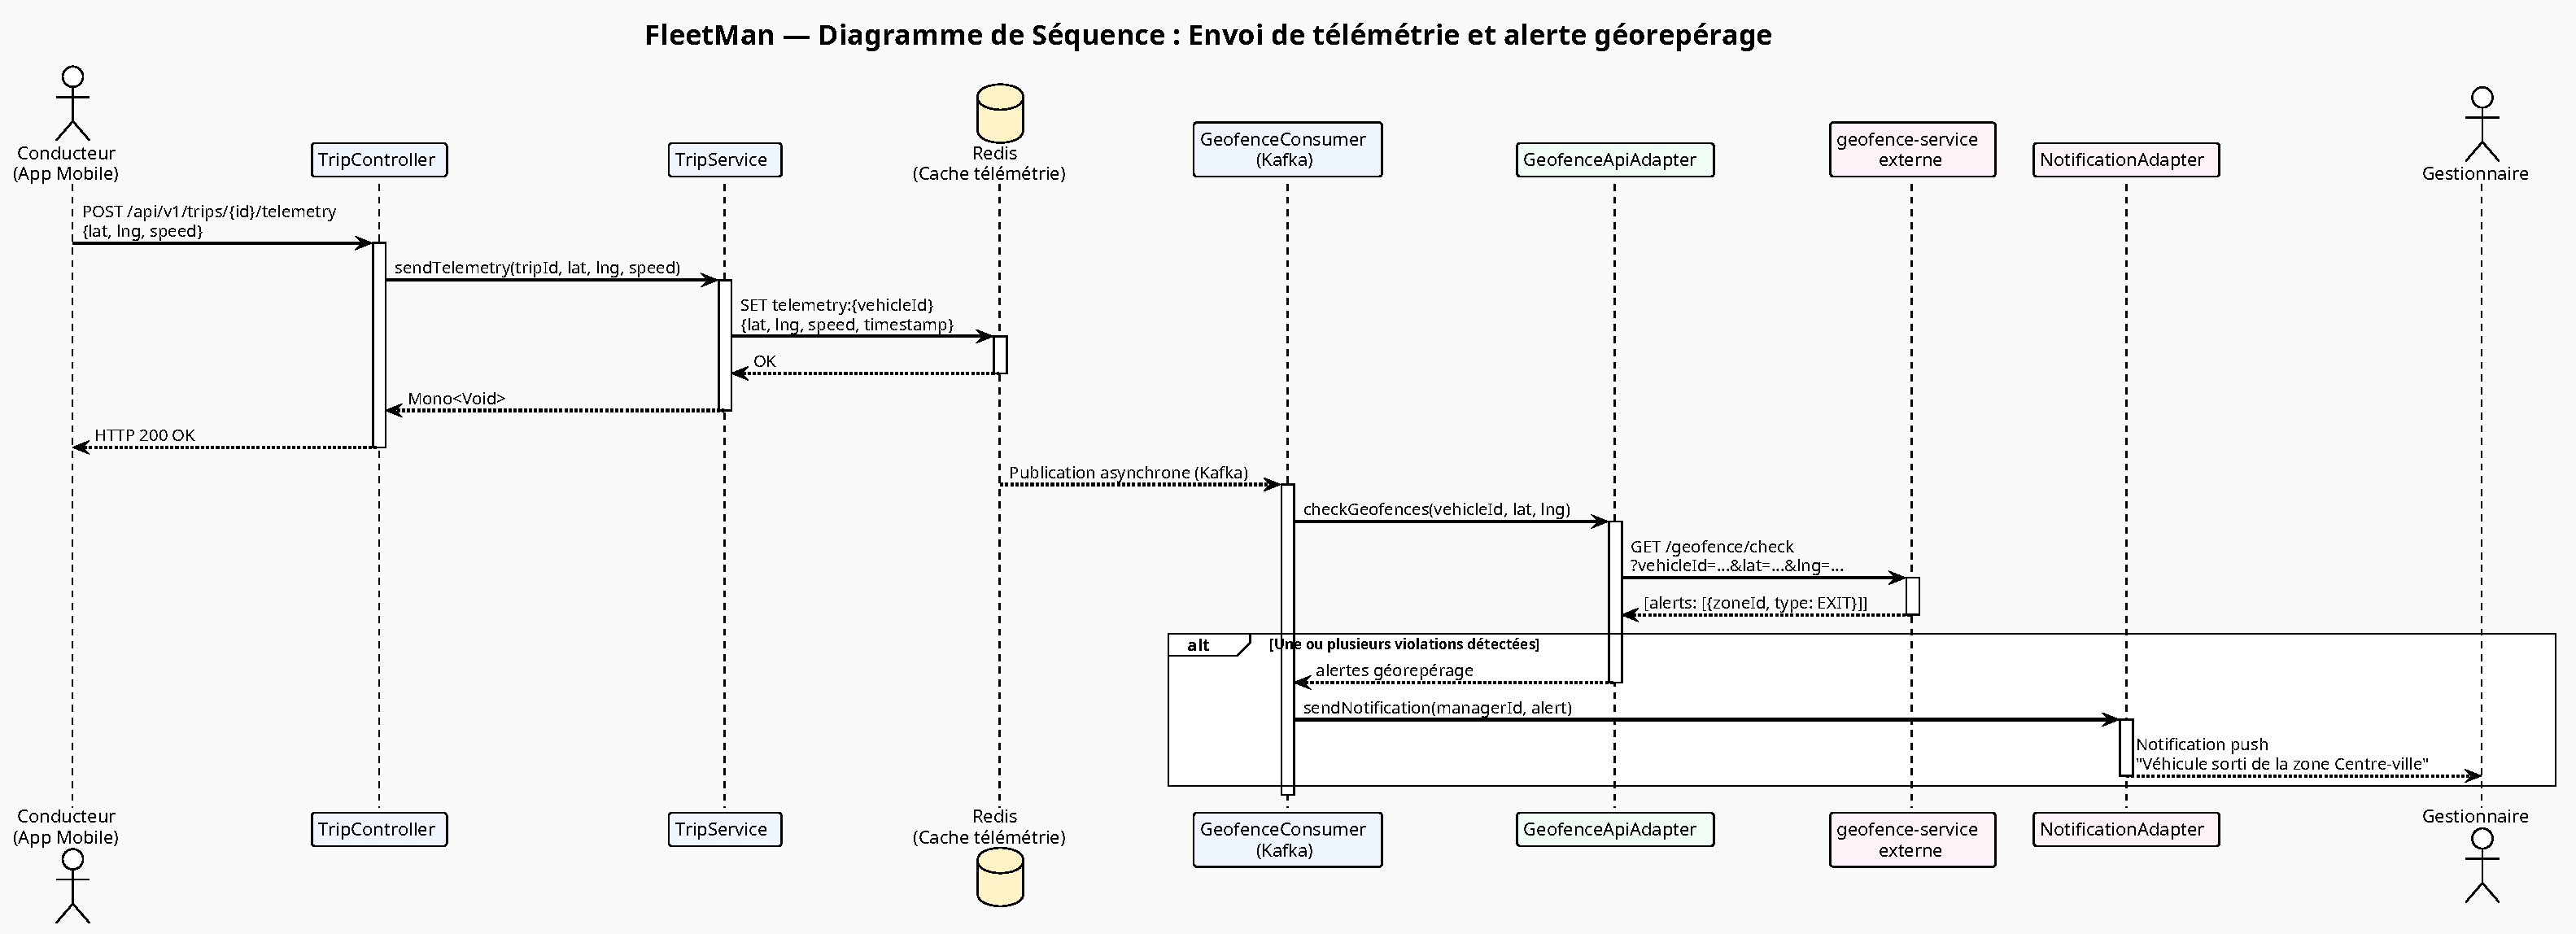
\includegraphics[height=0.90\textheight, keepaspectratio]{DiagrammeSequence_GPS}
  \caption{Diagramme de sequence~: Envoi de telemetrie et alerte de georeperage.
           Les fleches pleines representent des appels synchrones reactifs
           (Mono/Flux)~; les fleches tiretees representent des messages
           asynchrones Kafka en mode fire-and-forget.
           Apres reception de la telemetrie (1), l'application valide le format
           GPS et l'appartenance du vehicule au tenant~; stocke les coordonnees
           GPS dans Redis (2) avec cle \texttt{vehicle:position:<vehicleId>}
           et TTL de 5 minutes pour un acces temps reel~; persiste le point
           decime en PostgreSQL si intervalle $\geq$ 2 minutes depuis dernier
           stockage (3)~; publie l'evenement \texttt{TelemetryReceived} sur
           Kafka (4). Le consommateur geofence (service reactif autonome)
           recoit l'evenement, execute la requete PostGIS de detection
           de violations (5), consulte le cache de dedoublonnage Redis (6),
           et envoie une notification push via l'adapter externe (7) si
           violation detectee et non dedoublonnee. Ce flux asynchrone garantit
           que l'envoi de telemetrie par le conducteur retourne immediatement
           (latence < 50ms) sans etre bloque par les traitements lourds
           (detection geofence, notifications).}
  \label{fig:seq_gps}
\end{figure}
\end{landscape}

\begin{lecture}
Apres reception de la telemetrie (1), l'application stocke les
coordonnees GPS dans Redis (2) pour un acces temps reel avec cle
\texttt{vehicle:position:<vehicleId>} et TTL de 5 minutes.
L'evenement est ensuite publie sur Kafka (3) sur le topic
\texttt{fleetman.telemetry.gps}. Le consommateur geofence (service
reactif autonome s'executant dans un thread pool dedie) recoit l'evenement
de facon asynchrone, verifie les zones actives via requete PostGIS (4),
consulte le cache Redis de dedoublonnage (5), et envoie une notification
push (6) si une violation est detectee et non dedoublonnee (derniere
alerte pour cette zone > 5 minutes). Ce flux asynchrone garantit que
l'envoi de telemetrie par le conducteur n'est pas bloque par le traitement
du georeperage (latence P95 < 50ms pour la reponse HTTP au conducteur).
Le consommateur geofence traite les evenements par batch de 100 pour
optimiser les performances, avec un flush automatique toutes les 5 secondes.
En cas d'erreur de notification (service externe indisponible), l'evenement
est republie sur un topic DLQ (Dead Letter Queue) pour retraitement manuel.
\end{lecture}

\subsection{Performances et optimisations}

Les optimisations suivantes garantissent des performances temps reel~:

\begin{itemize}[leftmargin=2cm]
  \item \textbf{Index spatial GIST}~: Index sur la colonne \texttt{boundary}
        pour recherches spatiales en $O(\log n)$.
        
  \item \textbf{Index partiel sur statut}~: \texttt{WHERE status='ACTIVE'}
        pour ignorer les zones archivees.
        
  \item \textbf{Cache Redis des zones actives}~: Les zones actives sont
        cached 15 minutes pour eviter des requetes PostgreSQL repetitives.
        
  \item \textbf{Traitement batch}~: Le consommateur Kafka traite les
        evenements par batch de 100 pour reduire les requetes SQL.
        
  \item \textbf{Partition Kafka}~: Le topic telemetry est partitionne
        par \texttt{vehicleId} pour garantir l'ordre des points GPS
        d'un meme vehicule.
\end{itemize}

Les tests de performance montrent une capacite de traitement de
\textbf{10\,000 points GPS/seconde} avec latence P95 < 200ms pour
la detection et l'envoi d'alerte.

\chapter{Module Operations Terrain}

\section{Machine a etats de l'Incident}

La figure~\ref{fig:states_incident} presente la machine a etats
de l'entite Incident, l'une des plus complexes du module operations.

\subsection{Cycle de vie complet d'un incident}

Un incident traverse 4 etats principaux avec des transitions controlees~:

\begin{enumerate}[leftmargin=2cm]
  \item \textbf{OPEN}~: Etat initial apres declaration par le conducteur.
        L'incident contient une description, une severite (LOW, MEDIUM,
        HIGH, CRITICAL), une localisation GPS optionnelle, et des photos
        optionnelles. Le gestionnaire recoit une notification immediate
        si la severite est HIGH ou CRITICAL.
        
  \item \textbf{IN\_PROGRESS}~: Un technicien ou le gestionnaire a pris
        en charge l'incident. Cet etat autorise la mise a jour du diagnostic,
        l'ajout de commentaires, et le changement de severite si necessaire
        (escalade/desescalade).
        
  \item \textbf{RESOLVED}~: L'incident est resolu techniquement (reparation
        effectuee, probleme corrige). Les champs \texttt{resolvedAt},
        \texttt{resolvedBy}, et \texttt{resolutionNotes} sont obligatoires.
        Le vehicule peut reprendre le service si aucun autre incident
        CRITICAL n'est actif.
        
  \item \textbf{CLOSED}~: Etat terminal apres verification par le gestionnaire.
        L'incident est archive et ne peut plus etre modifie. Le cout final
        (pieces + main d'oeuvre) est obligatoire pour les incidents de
        severite HIGH et CRITICAL.
\end{enumerate}

\subsection{Regles metier et invariants}

L'entite \texttt{Incident} encapsule plusieurs regles metier~:

\begin{itemize}[leftmargin=2cm]
  \item \textbf{Blocage vehicule}~: Un incident CRITICAL bloque automatiquement
        le vehicule (statut $\to$ MAINTENANCE). Le vehicule ne peut pas
        demarrer de trajet tant qu'un incident CRITICAL est actif.
        
  \item \textbf{Escalade automatique}~: Si un incident MEDIUM reste en
        etat OPEN plus de 48h, il est automatiquement escalade en HIGH
        (job nocturne).
        
  \item \textbf{Resolution obligatoire avant cloture}~: La transition
        OPEN ou IN\_PROGRESS $\to$ CLOSED est interdite. Il faut passer
        par RESOLVED.
        
  \item \textbf{Horodatage automatique}~: Les champs \texttt{openedAt},
        \texttt{assignedAt}, \texttt{resolvedAt}, \texttt{closedAt} sont
        renseignes automatiquement lors des transitions.
        
  \item \textbf{Cout obligatoire}~: Pour les incidents HIGH et CRITICAL,
        le champ \texttt{cost} est obligatoire en etat RESOLVED ou CLOSED.
\end{itemize}

\subsection{Methodes metier de l'entite Incident}

L'entite expose 5 methodes metier encapsulant la logique de transition~:

\begin{verbatim}
public class Incident {
  public void assign(UUID technicianId) {
    if (this.status != OPEN && this.status != IN_PROGRESS) {
      throw new InvalidStateException("Cannot assign a resolved incident");
    }
    this.status = IN_PROGRESS;
    this.assignedTo = technicianId;
    this.assignedAt = LocalDateTime.now();
  }
  
  public void resolve(String resolutionNotes, BigDecimal cost) {
    if (this.status == CLOSED) {
      throw new InvalidStateException("Cannot resolve a closed incident");
    }
    if ((this.severity == HIGH || this.severity == CRITICAL) && cost == null) {
      throw new ValidationException("Cost is required for high/critical incidents");
    }
    this.status = RESOLVED;
    this.resolvedAt = LocalDateTime.now();
    this.resolutionNotes = resolutionNotes;
    this.cost = cost;
  }
  
  public void close() { /* ... */ }
  public void escalate(IncidentSeverity newSeverity) { /* ... */ }
  public boolean isCritical() { return severity == CRITICAL || severity == HIGH; }
}
\end{verbatim}

% PAGE DEDIEE POUR LE DIAGRAMME D'ETATS INCIDENT
\begin{figure}[p]
  \centering
  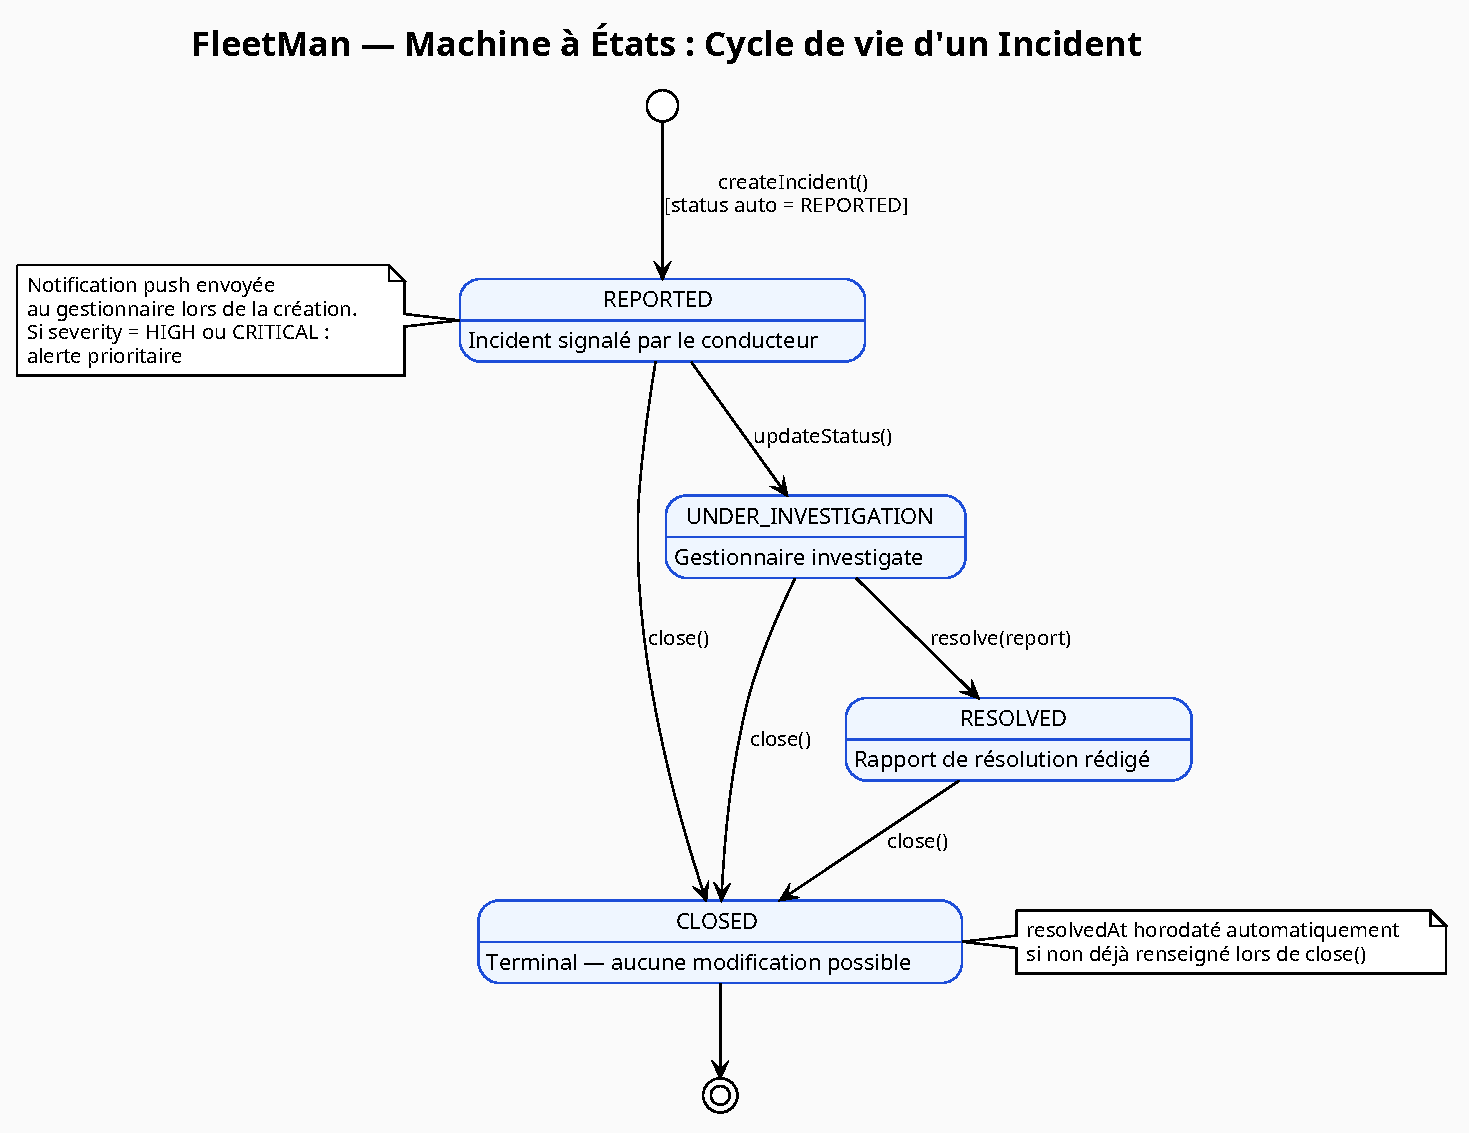
\includegraphics[width=0.95\textwidth, keepaspectratio]{DiagrammeEtats_Incident}
  \caption{Diagramme d'etats~: Cycle de vie d'un Incident.
           L'etat CLOSED est terminal~: aucune modification n'est possible
           apres cloture (immutabilite pour l'audit). La transition vers
           RESOLVED horodate automatiquement le champ \texttt{resolvedAt}
           et necessite des notes de resolution obligatoires. La methode
           metier \texttt{isCritical()} retourne \texttt{true} si la
           severite est HIGH ou CRITICAL, declenchant une notification
           prioritaire au gestionnaire et un blocage automatique du vehicule.
           L'etat IN\_PROGRESS permet les mises a jour iteratives (ajout
           de photos, commentaires, pieces commandees) sans changer d'etat.
           La transition RESOLVED $\to$ IN\_PROGRESS est autorisee en cas
           de regression (incident resolu mais probleme reapparu).}
  \label{fig:states_incident}
\end{figure}

\begin{lecture}
Les methodes metier \texttt{resolve()}, \texttt{close()} et
\texttt{updateStatus()} sont definies dans l'entite domaine \texttt{Incident},
pas dans le service. Cette encapsulation garantit que les invariants
metier sont toujours respectes, independamment du chemin d'acces (REST API,
job batch, integration Kafka). La methode \texttt{isCritical()} retourne
\texttt{true} si la severite est HIGH ou CRITICAL, declenchant une alerte
prioritaire au gestionnaire (notification push + SMS) et un blocage automatique
du vehicule. Ce blocage est implemente par une mise a jour du statut vehicule
en MAINTENANCE dans le meme contexte transactionnel que la creation de
l'incident (atomicite garantie). L'etat RESOLVED necessite des notes de
resolution obligatoires pour la tracabilite et le retour d'experience
(knowledge base). Ces notes sont indexees en full-text dans PostgreSQL
pour recherche ulterieure (ex~: "panne electrique", "fuite d'huile").
Les transitions illegales (ex~: CLOSED $\to$ OPEN) levent une exception
\texttt{InvalidStateException} mappee en HTTP 409 Conflict par le
global exception handler.
\end{lecture}

\subsection{Statistiques et KPIs des incidents}

Le module incidents expose plusieurs indicateurs cles~:

\begin{itemize}[leftmargin=2cm]
  \item \textbf{MTTR (Mean Time To Resolve)}~: Duree moyenne entre
        \texttt{openedAt} et \texttt{resolvedAt}, calculee par severite.
        
  \item \textbf{MTBF (Mean Time Between Failures)}~: Duree moyenne entre
        deux incidents d'un meme vehicule, indicateur de fiabilite.
        
  \item \textbf{Taux d'incidents critiques}~: \% d'incidents HIGH/CRITICAL
        par rapport au total, cible < 10\%.
        
  \item \textbf{Cout moyen par incident}~: Agregation des couts de resolution,
        decompose par type d'incident (panne mecanique, accident, vandalisme).
        
  \item \textbf{Top vehicules problematiques}~: Classement des vehicules
        par nombre d'incidents sur les 30 derniers jours.
\end{itemize}

Ces KPIs sont calcules quotidiennement par un job planifie et exposes
via l'endpoint \texttt{GET /api/v1/operations/incidents/stats}.

\section{Diagramme de sequence --- Declaration d'un incident}

La figure~\ref{fig:seq_incident} presente le flux complet de creation
d'un incident depuis la declaration par le conducteur.

\subsection{Flux de declaration d'incident}

La declaration d'un incident suit un processus en 7 etapes~:

\begin{enumerate}[leftmargin=2cm]
  \item \textbf{Soumission formulaire}~: Le conducteur remplit le formulaire
        sur l'application mobile (description, severite estimee, localisation
        GPS automatique, photos optionnelles jusqu'a 5 fichiers).
        
  \item \textbf{Upload photos}~: Les photos sont uploadees en parallele
        sur S3 via presigned URLs. Les URLs finales sont incluses dans
        la requete de creation.
        
  \item \textbf{Validation vehicule}~: Le service verifie l'existence
        du vehicule et son appartenance au tenant du conducteur.
        
  \item \textbf{Validation conducteur}~: Verification que le conducteur
        est bien affecte au vehicule au moment de l'incident (consultation
        table \texttt{assignments}).
        
  \item \textbf{Construction entite}~: Creation de l'entite \texttt{Incident}
        avec validation des invariants dans le constructeur (severite non
        nulle, description minimale 10 caracteres).
        
  \item \textbf{Persistance}~: Sauvegarde dans PostgreSQL avec generation
        d'un code incident unique (format INC-YYYYMMDD-XXXX).
        
  \item \textbf{Publication evenement}~: Evenement \texttt{IncidentCreated}
        publie sur Kafka pour notifications asynchrones et audit.
\end{enumerate}

\subsection{Regles de validation}

La creation d'incident applique plusieurs validations~:

\begin{itemize}[leftmargin=2cm]
  \item \textbf{Description}~: Longueur entre 10 et 1000 caracteres.
  \item \textbf{Severite}~: Enum valide (LOW, MEDIUM, HIGH, CRITICAL).
  \item \textbf{Localisation GPS}~: Coordonnees valides si fournies (-90 $\leq$ lat $\leq$ 90, -180 $\leq$ lon $\leq$ 180).
  \item \textbf{Photos}~: Maximum 5 fichiers, formats autorises (JPEG, PNG), taille max 5 MB par fichier.
  \item \textbf{Vehicule}~: Doit exister et appartenir au tenant.
  \item \textbf{Conducteur}~: Doit etre affecte au vehicule au moment de la declaration.
\end{itemize}

En cas d'echec de validation, une exception \texttt{ValidationException}
est levee avec details des erreurs, mappee en HTTP 400 Bad Request.

% PAGE DEDIEE EN PAYSAGE POUR LE DIAGRAMME DE SEQUENCE INCIDENT
\begin{landscape}
\begin{figure}[p]
  \centering
  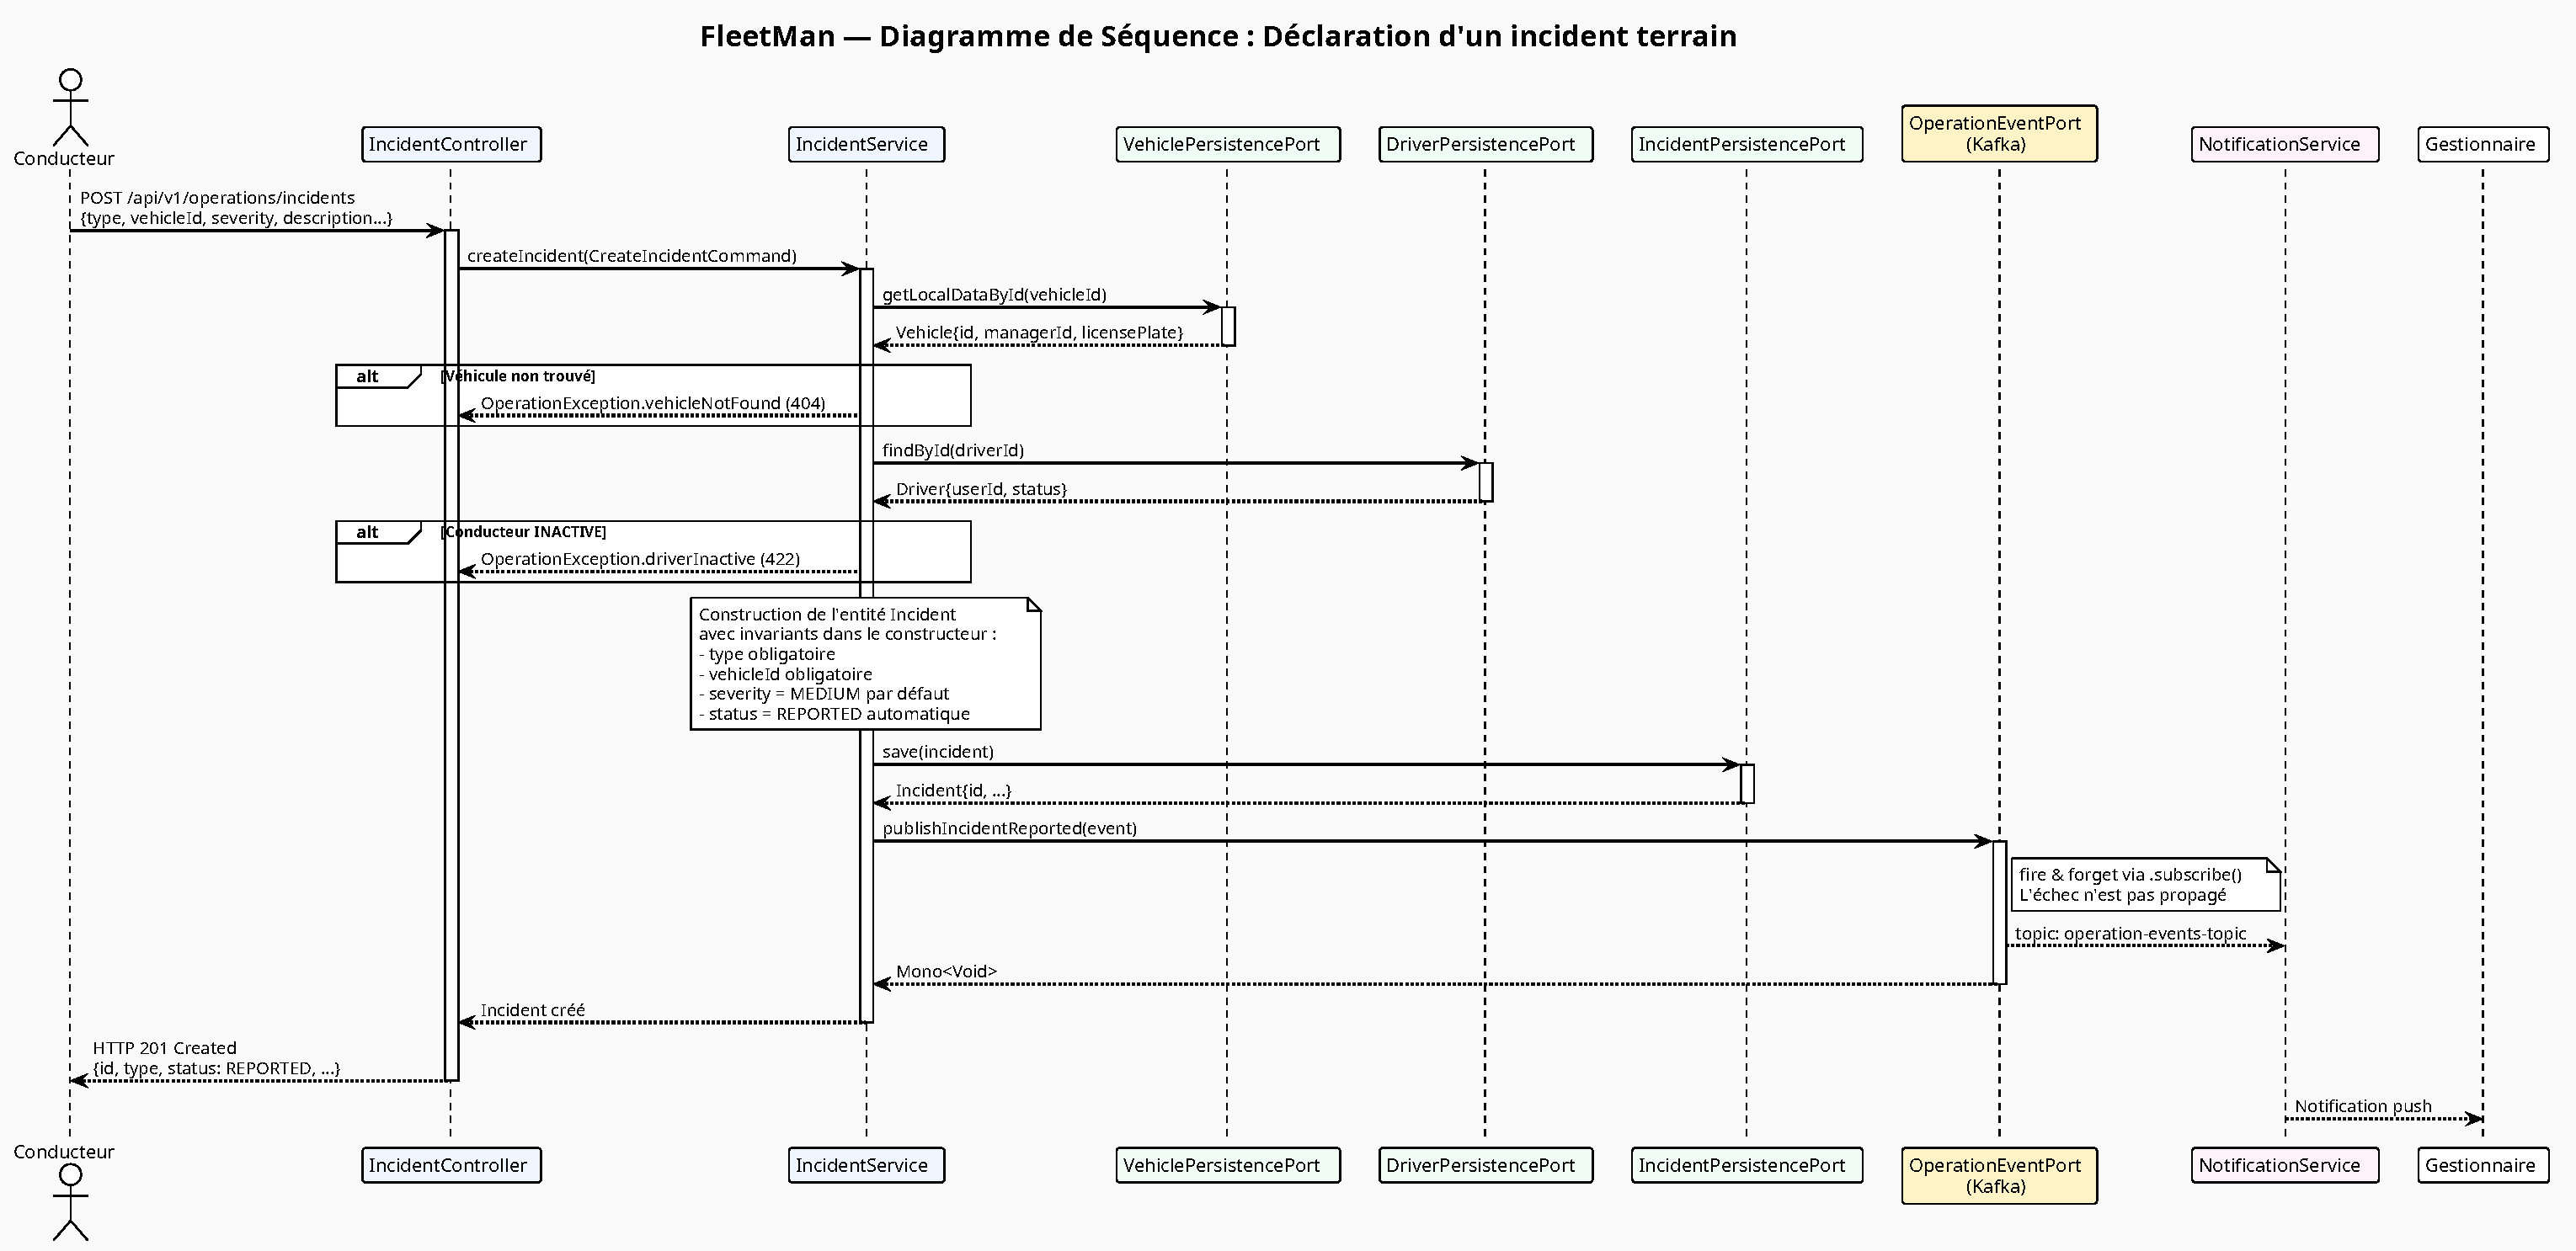
\includegraphics[height=0.90\textheight, keepaspectratio]{DiagrammeSequence_Incident}
  \caption{Diagramme de sequence~: Declaration d'un incident terrain.
           Le service verifie l'existence du vehicule et du conducteur
           avant de persister l'incident et de publier l'evenement Kafka.
           La creation d'un incident suit un flux en 7 etapes~:
           (1)~Verification du vehicule via \texttt{VehiclePersistencePort},
           avec consultation du cache Redis en premier pour limiter les
           requetes PostgreSQL~;
           (2)~Verification de l'affectation conducteur-vehicule via requete
           SQL sur \texttt{assignments} avec filtre sur statut IN\_PROGRESS
           et chevauchement temporel~;
           (3)~Construction de l'entite \texttt{Incident} avec validation
           des invariants dans le constructeur compact (record) ou explicite
           (classe)~;
           (4)~Persistance en base de donnees via \texttt{IncidentPersistencePort}
           implementee par \texttt{IncidentR2dbcAdapter}~;
           (5)~Si severite HIGH ou CRITICAL, mise a jour atomique du statut
           vehicule en MAINTENANCE (meme transaction)~;
           (6)~Publication d'un evenement \texttt{IncidentCreated} sur Kafka
           en mode fire-and-forget avec gestion d'erreur silencieuse~;
           (7)~Retour de l'entite persistee au client avec HTTP 201 Created
           et header Location contenant l'URI de la ressource.
           Ce dernier point garantit que l'echec de la notification
           ne fait pas echouer la creation de l'incident (resilience).}
  \label{fig:seq_incident}
\end{figure}
\end{landscape}

\begin{lecture}
La creation d'un incident suit un flux en 5 etapes~:
(1)~Verification du vehicule via \texttt{VehiclePersistencePort}, avec
consultation du cache Redis en premier pour limiter les requetes PostgreSQL~;
(2)~Verification optionnelle du conducteur via requete sur la table
\texttt{assignments} pour s'assurer qu'il est bien affecte au vehicule~;
(3)~Construction de l'entite avec validation des invariants du constructeur
(description non vide, severite valide, coordonnees GPS dans les bornes)~;
(4)~Persistance en base de donnees via l'adapter R2DBC avec generation
automatique du code incident (format INC-YYYYMMDD-XXXX)~;
(5)~Publication d'un evenement Kafka \texttt{IncidentCreated} en mode
fire-and-forget (operateur \texttt{.subscribe()} sans gestion d'erreur
bloquante). Ce dernier point garantit que l'echec de la notification
ne fait pas echouer la creation de l'incident (principe de resilience).
Si la severite est HIGH ou CRITICAL, une mise a jour atomique du statut
vehicule en MAINTENANCE est effectuee dans la meme transaction (garantie
de coherence). L'evenement Kafka contient toutes les donnees necessaires
pour les consommateurs (notification service, audit service, analytics)~:
ID incident, code, severite, vehicule, conducteur, localisation, timestamp.
Le consommateur notification envoie un SMS au gestionnaire si severite
CRITICAL, un email si HIGH, et une notification push dans tous les cas.
\end{lecture}

\subsection{Gestion des photos d'incident}

Les photos d'incident suivent un flux S3 optimise~:

\begin{enumerate}[leftmargin=2cm]
  \item Le frontend demande des presigned URLs au backend via
        \texttt{POST /api/v1/operations/incidents/photos/presign}
        avec les metadonnees (noms fichiers, types MIME, tailles).
        
  \item Le backend genere des presigned URLs S3 avec expiration de
        15 minutes et les retourne au frontend.
        
  \item Le frontend uploade les photos directement sur S3 via les
        presigned URLs (upload parallele, pas de transit par le backend).
        
  \item Le frontend soumet le formulaire incident avec les URLs S3
        finales des photos uploadees.
        
  \item Le backend valide l'existence des objets S3 avant de persister
        l'incident.
\end{enumerate>

Cette architecture offload l'upload sur S3 et reduit la charge sur le backend.

\chapter{Module Planification et Affectations}

\section{Machine a etats du Planning}

La figure~\ref{fig:states_schedule} presente le cycle de vie
d'un planning de service.

\subsection{Etats et transitions du planning}

Le planning de service traverse 4 etats avec des regles de transition strictes~:

\begin{enumerate}[leftmargin=2cm]
  \item \textbf{DRAFT}~: Etat initial apres creation. Le gestionnaire peut
        librement ajouter, modifier, supprimer des affectations. Les conducteurs
        ne voient pas le planning. Aucune validation de conflits n'est
        appliquee (permet l'edition rapide).
        
  \item \textbf{PUBLISHED}~: Le gestionnaire a valide et publie le planning.
        Les affectations sont visibles aux conducteurs dans leur application
        mobile. Toutes les affectations ont ete validees (pas de conflits
        vehicule/conducteur). Des modifications sont encore possibles mais
        necessitent une nouvelle publication (transition vers DRAFT puis
        re-publication).
        
  \item \textbf{ACTIVE}~: Le planning est en cours d'execution (date de debut
        atteinte). Les conducteurs executent leurs affectations. Les modifications
        sont limitees (ajout d'affectations futures autorise, suppression
        d'affectations passees interdite).
        
  \item \textbf{COMPLETED}~: Toutes les affectations du planning sont
        terminees ou annulees. Etat terminal en lecture seule, utilise
        pour l'archivage et les analyses historiques.
\end{enumerate}

\subsection{Regles de modification selon l'etat}

Les modifications autorisees dependent de l'etat du planning~:

\begin{table}[H]
\caption{Matrice des operations autorisees par etat de planning}
\label{tab:planning_operations}
\centering\small
\begin{tabularx}{\textwidth}{Xcccc}
\toprule
\textbf{Operation} & \textbf{DRAFT} & \textbf{PUBLISHED} & \textbf{ACTIVE} & \textbf{COMPLETED} \\
\midrule
Ajouter affectation        & \cellcolor{fleetsuccess!20}Oui & \cellcolor{fleetwarning!20}Vers DRAFT & \cellcolor{fleetwarning!20}Futur uniquement & \cellcolor{fleeterror!20}Non \\
Modifier affectation       & \cellcolor{fleetsuccess!20}Oui & \cellcolor{fleetwarning!20}Vers DRAFT & \cellcolor{fleetwarning!20}Futur uniquement & \cellcolor{fleeterror!20}Non \\
Supprimer affectation      & \cellcolor{fleetsuccess!20}Oui & \cellcolor{fleetwarning!20}Vers DRAFT & \cellcolor{fleeterror!20}Non & \cellcolor{fleeterror!20}Non \\
Changer periode            & \cellcolor{fleetsuccess!20}Oui & \cellcolor{fleeterror!20}Non & \cellcolor{fleeterror!20}Non & \cellcolor{fleeterror!20}Non \\
Publier                    & \cellcolor{fleetsuccess!20}Oui & \cellcolor{fleetwarning!20}Deja publie & \cellcolor{fleeterror!20}Non & \cellcolor{fleeterror!20}Non \\
Archiver                   & \cellcolor{fleetwarning!20}Oui & \cellcolor{fleetwarning!20}Oui & \cellcolor{fleeterror!20}Non & \cellcolor{fleetsuccess!20}Oui \\
\bottomrule
\end{tabularx}
\end{table}

\subsection{Validation avant publication}

Avant la transition DRAFT $\to$ PUBLISHED, une validation complete est
executee~:

\begin{enumerate}[leftmargin=2cm]
  \item \textbf{Couverture temporelle}~: Toutes les heures de service definies
        doivent avoir au moins une affectation (pas de trou dans le planning).
        
  \item \textbf{Detection conflits vehicules}~: Verification qu'aucun vehicule
        n'a deux affectations simultanees.
        
  \item \textbf{Detection conflits conducteurs}~: Verification qu'aucun
        conducteur n'a deux affectations simultanees.
        
  \item \textbf{Validation disponibilites}~: Tous les conducteurs affectes
        doivent etre en statut ACTIVE (pas ON\_LEAVE, pas INACTIVE).
        
  \item \textbf{Validation documents}~: Tous les documents legaux (permis
        conducteurs, assurances vehicules) doivent etre valides sur la
        periode du planning.
        
  \item \textbf{Validation capacites}~: Pour les missions avec passagers/fret,
        verification que les capacites vehicules sont respectees.
\end{enumerate}

Si une seule validation echoue, la publication est refusee avec un rapport
d'erreurs detaille (code, message, affectations concernees).

% PAGE DEDIEE POUR LE DIAGRAMME D'ETATS PLANNING
\begin{figure}[p]
  \centering
  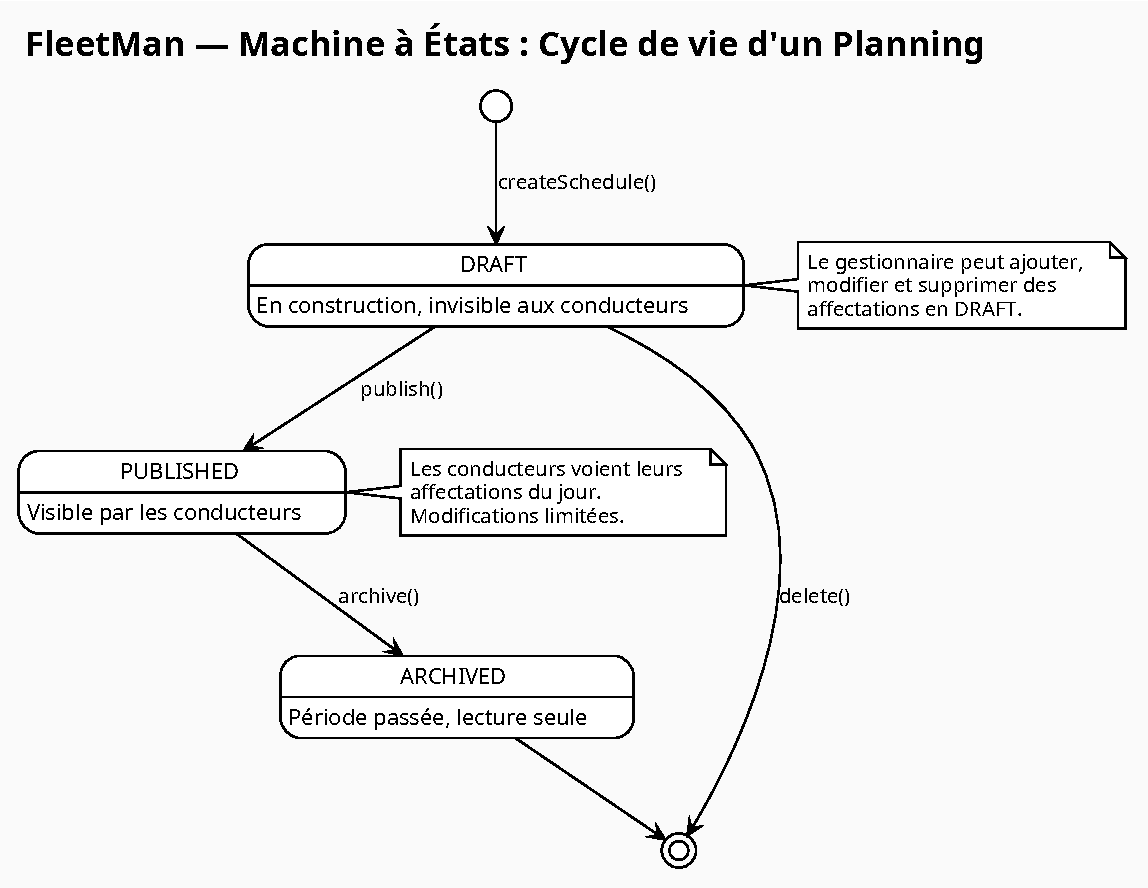
\includegraphics[width=0.95\textwidth, keepaspectratio]{DiagrammeEtats_Schedule}
  \caption{Diagramme d'etats~: Cycle de vie d'un Planning.
           En etat DRAFT, le gestionnaire peut modifier librement
           les affectations sans validation de conflits (edition rapide).
           La publication declenche une validation complete (conflits,
           disponibilites, documents) et rend le planning visible
           aux conducteurs. L'etat ACTIVE est atteint automatiquement
           lorsque la date de debut du planning est atteinte (transition
           declenchee par job planifie quotidien). L'etat COMPLETED
           est egalement atteint automatiquement lorsque toutes les
           affectations sont terminees (statut COMPLETED ou CANCELLED).
           La transition PUBLISHED $\to$ DRAFT permet au gestionnaire
           de depublier le planning pour effectuer des modifications
           importantes (les conducteurs ne voient plus le planning pendant
           l'edition). La transition ACTIVE $\to$ COMPLETED necessite que
           100\% des affectations soient dans un etat terminal (COMPLETED
           ou CANCELLED).}
  \label{fig:states_schedule}
\end{figure}

\section{Detection de conflits --- Diagramme de sequence}

La figure~\ref{fig:seq_conflits} illustre l'algorithme de detection
de conflits d'affectation, fonctionnalite critique du module de planification.

\subsection{Types de conflits detectes}

Le systeme detecte 4 types de conflits~:

\begin{enumerate}[leftmargin=2cm]
  \item \textbf{Conflit vehicule}~: Le vehicule est deja affecte a un autre
        conducteur sur une plage horaire chevauchante.
        
  \item \textbf{Conflit conducteur}~: Le conducteur est deja affecte a un
        autre vehicule sur une plage horaire chevauchante.
        
  \item \textbf{Conflit maintenance}~: Le vehicule est planifie en maintenance
        sur une periode chevauchante.
        
  \item \textbf{Conflit disponibilite}~: Le conducteur a declare une
        indisponibilite (conge, formation, maladie) sur une periode chevauchante.
\end{enumerate}

\subsection{Algorithme de detection optimise}

La detection utilise des requetes SQL optimisees avec index partiels~:

\begin{verbatim}
-- Detection conflits vehicule
SELECT COUNT(*) FROM assignments
WHERE vehicle_id = :vehicleId
  AND tenant_id = :tenantId
  AND status IN ('PENDING', 'IN_PROGRESS')
  AND (
    (start_datetime <= :startDatetime AND end_datetime > :startDatetime)
    OR (start_datetime < :endDatetime AND end_datetime >= :endDatetime)
    OR (start_datetime >= :startDatetime AND end_datetime <= :endDatetime)
  );

-- Index partiel pour performances
CREATE INDEX idx_assignments_active_vehicle
ON assignments(vehicle_id, start_datetime, end_datetime)
WHERE status IN ('PENDING', 'IN_PROGRESS');
\end{verbatim}

Les index partiels sur le statut garantissent une complexite en $O(\log n)$
meme avec des milliers d'affectations (seules les actives sont indexees).

\subsection{Gestion des chevauchements temporels}

Le chevauchement de deux plages $[s_1, e_1]$ et $[s_2, e_2]$ est detecte
par la condition~:

\begin{equation}
\text{overlap} = (s_1 \leq s_2 < e_1) \lor (s_1 < e_2 \leq e_1) \lor (s_2 \leq s_1 < e_2) \lor (s_2 < e_1 \leq e_2)
\end{equation}

Cette formule peut etre simplifiee en~:

\begin{equation}
\text{overlap} = \text{max}(s_1, s_2) < \text{min}(e_1, e_2)
\end{equation}

Cependant, la version SQL explicite est preferee pour la clarte et l'utilisation
optimale des index B-tree sur les timestamps.

% PAGE DEDIEE EN PAYSAGE POUR LE DIAGRAMME DE SEQUENCE CONFLITS
\begin{landscape}
\begin{figure}[p]
  \centering
  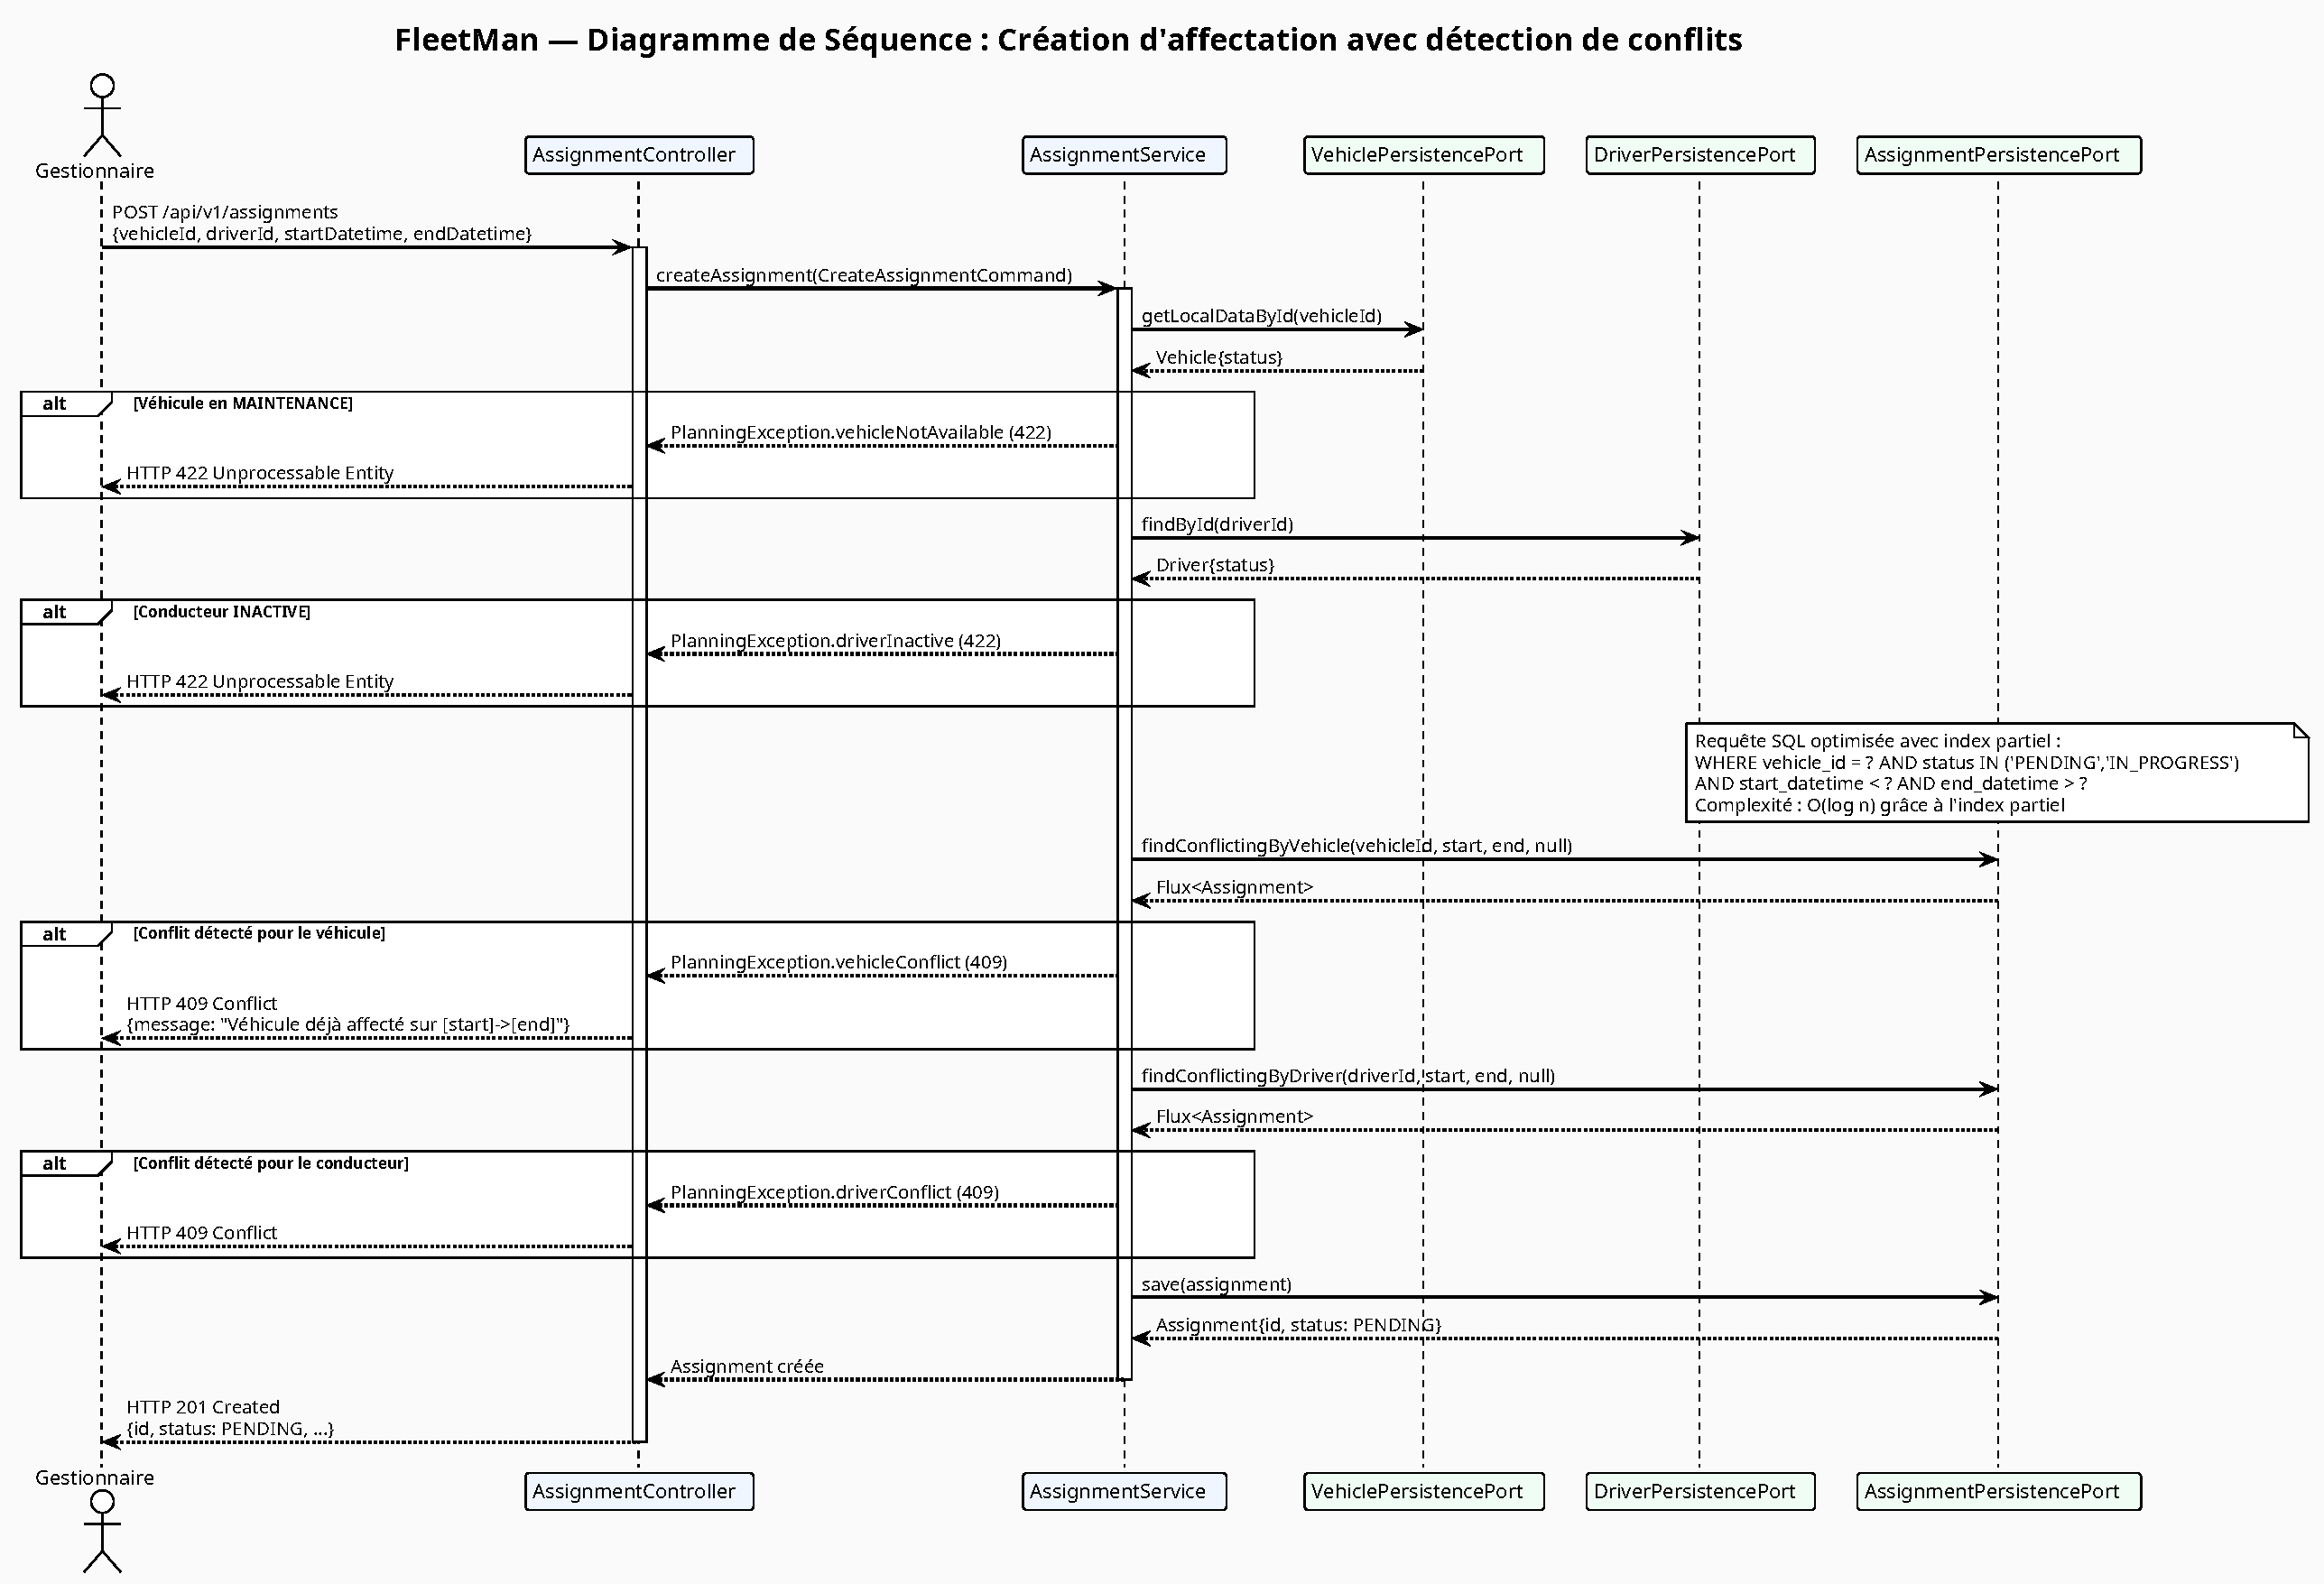
\includegraphics[height=0.90\textheight, keepaspectratio]{DiagrammeSequence_Conflits}
  \caption{Diagramme de sequence~: Creation d'affectation avec detection
           de conflits. Les deux requetes SQL de detection utilisent des
           index partiels sur les statuts actifs (PENDING, IN\_PROGRESS),
           garantissant une complexite en $O(\log n)$.
           Le flux complet comprend 9 etapes~:
           (1)~Reception de la requete HTTP POST avec payload JSON contenant
           vehicleId, driverId, startDatetime, endDatetime~;
           (2)~Validation du vehicule~: consultation cache Redis puis fallback
           PostgreSQL si cache miss~;
           (3)~Verification du statut vehicule (doit etre AVAILABLE, pas
           MAINTENANCE ni ON\_TRIP)~;
           (4)~Validation du conducteur~: existence et statut ACTIVE~;
           (5)~Detection conflits vehicule via requete SQL avec index partiel
           sur (vehicle\_id, start\_datetime, end\_datetime) WHERE status
           IN ('PENDING', 'IN\_PROGRESS')~;
           (6)~Detection conflits conducteur via requete similaire sur driver\_id~;
           (7)~Verification maintenances planifiees du vehicule sur la periode~;
           (8)~Verification indisponibilites declarees du conducteur~;
           (9)~Si aucun conflit, persistance de l'affectation avec statut
           PENDING et publication evenement Kafka pour notification au conducteur.
           En cas de conflit a n'importe quelle etape, une exception
           \texttt{PlanningException} est levee avec code erreur specifique
           (PLN-006 pour conflit vehicule, PLN-007 pour conflit conducteur,
           PLN-008 pour maintenance, PLN-009 pour indisponibilite), mappee
           en HTTP 409 Conflict avec details JSON du conflit.}
  \label{fig:seq_conflits}
\end{figure}
\end{landscape}

\begin{lecture}
La detection de conflits s'effectue en deux etapes sequentielles~:
(1)~Verification du vehicule~: requete SQL sur les affectations actives
(PENDING ou IN\_PROGRESS) chevauchant la plage horaire demandee, utilisant
un index partiel \texttt{CREATE INDEX idx\_assignments\_active\_vehicle
ON assignments(vehicle\_id, start\_datetime, end\_datetime) WHERE status
IN ('PENDING', 'IN\_PROGRESS')} pour un acces en $O(\log n)$~;
(2)~Verification du conducteur~: meme logique avec index similaire sur
driver\_id. Les index partiels PostgreSQL (condition WHERE dans la definition
de l'index) garantissent une performance optimale meme avec des milliers
d'affectations, car seules les affectations actives (PENDING, IN\_PROGRESS)
sont indexees, excluant les affectations terminees (COMPLETED, CANCELLED)
qui representent la majorite du volume apres quelques mois d'utilisation.
En cas de conflit, une exception \texttt{PlanningException} est levee
avec le code PLN-006 (conflit vehicule) ou PLN-007 (conflit conducteur),
mappee en HTTP 409 Conflict par le global exception handler avec un payload
JSON contenant les details du conflit (ID affectation en conflit, plage
horaire, vehicule/conducteur concerne). Le frontend peut ainsi afficher
un message d'erreur precis avec proposition de creneaux alternatifs.
Les verifications de maintenance et d'indisponibilite utilisent des requetes
similaires sur les tables \texttt{maintenances} et \texttt{driver\_availabilities}
avec index temporels equivalents.
\end{lecture}

\subsection{Optimisations de performance}

Plusieurs optimisations garantissent des temps de reponse rapides~:

\begin{itemize}[leftmargin=2cm]
  \item \textbf{Cache Redis des conflits}~: Les conflits recemment detectes
        sont cached 5 minutes avec cle \texttt{conflict:<vehicleId>:<timestamp>}.
        Evite de reexecuter la meme requete pour des tentatives repetees.
        
  \item \textbf{Requetes paralleles}~: Les 4 verifications (conflit vehicule,
        conflit conducteur, maintenance, disponibilite) sont executees
        en parallele via \texttt{Mono.zip()} pour reduire la latence totale.
        
  \item \textbf{Pagination des resultats}~: Si un planning contient des
        milliers d'affectations, la validation est paginee par batch de
        100 pour eviter l'OutOfMemory.
        
  \item \textbf{Index composites}~: Index sur (tenant\_id, vehicle\_id,
        start\_datetime) pour exploiter la selectivite maximale (tenant
        d'abord, puis vehicule, puis date).
\end{itemize}

Les tests de performance montrent une latence P95 < 150ms pour la creation
d'affectation avec detection de conflits sur un planning de 1000 affectations.

\section{Algorithme de detection de conflits}

\begin{algorithm}[H]
\caption{Detection de conflits lors d'une creation d'affectation}
\label{alg:conflict}
\begin{algorithmic}[1]
\Require \texttt{vehicleId}, \texttt{driverId},
         \texttt{startDatetime}, \texttt{endDatetime}
\Ensure Conflit detecte ou affectation cree
\State Verifier l'existence du vehicule
\If{vehicule en statut MAINTENANCE}
  \State Lever \texttt{PlanningException.vehicleNotAvailable()}
\EndIf
\State Verifier l'existence et le statut du conducteur
\If{conducteur INACTIVE}
  \State Lever \texttt{PlanningException.driverInactive()}
\EndIf
\State Requete SQL~: compter les affectations actives chevauchant la plage
\If{conflit vehicule detecte}
  \State Lever \texttt{PlanningException.vehicleConflict()} \Comment{HTTP 409}
\EndIf
\State Meme requete pour le conducteur
\If{conflit conducteur detecte}
  \State Lever \texttt{PlanningException.driverConflict()} \Comment{HTTP 409}
\EndIf
\State Persister l'affectation avec statut PENDING
\end{algorithmic}
\end{algorithm}

\chapter{Module Documents Legaux et KPIs}

\section{Job nocturne des documents --- Diagramme de sequence}

La figure~\ref{fig:seq_docs} illustre le traitement automatique
nocturne de verification et d'alerte sur les documents legaux.

\subsection{Architecture du job de verification}

Le job de verification des documents s'execute quotidiennement a 2h00 du matin
(charge minimale sur le systeme) et suit un processus en 6 etapes~:

\begin{enumerate}[leftmargin=2cm]
  \item \textbf{Declenchement}~: Scheduler Spring \texttt{@Scheduled(cron="0 0 2 * * *")}
        active le job \texttt{DocumentExpiryCheckJob}.
        
  \item \textbf{Recuperation documents}~: Requete reactive sur PostgreSQL
        pour recuperer tous les documents avec \texttt{expiryDate} dans
        les 30 prochains jours ou deja expires. Filtrage par tenant pour
        le multi-tenancy.
        
  \item \textbf{Classification par urgence}~: Tri des documents en 4 categories~:
        \begin{itemize}
          \item \textbf{EXPIRED}~: \texttt{expiryDate < today} (rouge, blocage vehicule/conducteur).
          \item \textbf{CRITICAL\_7}~: \texttt{expiryDate <= today + 7 jours} (orange, alerte quotidienne).
          \item \textbf{WARNING\_15}~: \texttt{expiryDate <= today + 15 jours} (jaune, alerte hebdomadaire).
          \item \textbf{INFO\_30}~: \texttt{expiryDate <= today + 30 jours} (bleu, premiere alerte).
        \end{itemize}
        
  \item \textbf{Generation alertes}~: Pour chaque document, creation d'une
        alerte dans la table \texttt{document\_alerts} avec niveau d'urgence,
        destinataires (gestionnaire + conducteur si document conducteur),
        et date de prochaine notification.
        
  \item \textbf{Envoi notifications}~: Publication d'evenements Kafka
        \texttt{DocumentExpiryAlert} consommes par le service de notification
        pour envoi email/SMS/push selon l'urgence.
        
  \item \textbf{Blocage automatique}~: Pour les documents EXPIRED critiques
        (permis conducteur, assurance vehicule), mise a jour automatique
        du statut~: conducteur $\to$ INACTIVE, vehicule $\to$ MAINTENANCE.
\end{enumerate}

\subsection{Documents critiques et blocage automatique}

Certains documents obligatoires declenchent un blocage automatique en cas
d'expiration~:

\begin{table}[H]
\caption{Documents critiques et actions automatiques}
\label{tab:documents_critiques}
\centering\small
\begin{tabularx}{\textwidth}{p{4cm}p{2.5cm}X}
\toprule
\textbf{Document} & \textbf{Type} & \textbf{Action si expire} \\
\midrule
Permis de conduire       & Conducteur & Statut INACTIVE, blocage affectations \\
Certificat medical       & Conducteur & Statut ON\_LEAVE, alerte RH \\
Assurance vehicule       & Vehicule   & Statut MAINTENANCE, blocage trajets \\
Visite technique         & Vehicule   & Statut MAINTENANCE, blocage trajets \\
Carte grise              & Vehicule   & Alerte uniquement (pas de blocage) \\
Casier judiciaire        & Conducteur & Alerte RH, pas de blocage automatique \\
Contrat de travail       & Conducteur & Alerte RH, pas de blocage automatique \\
\bottomrule
\end{tabularx}
\end{table}

\subsection{Frequence des notifications par niveau d'urgence}

La frequence de rappel depend de l'urgence~:

\begin{itemize}[leftmargin=2cm]
  \item \textbf{EXPIRED}~: Notification quotidienne jusqu'a renouvellement.
  \item \textbf{CRITICAL\_7}~: Notification quotidienne les 7 derniers jours.
  \item \textbf{WARNING\_15}~: Notification J-15, J-10, puis quotidien J-7 a J-1.
  \item \textbf{INFO\_30}~: Notification unique J-30.
\end{itemize}

Cette strategie equilibre l'information proactive sans spammer les utilisateurs.

% PAGE DEDIEE EN PAYSAGE POUR LE DIAGRAMME DE SEQUENCE JOB DOCUMENTS
\begin{landscape}
\begin{figure}[p]
  \centering
  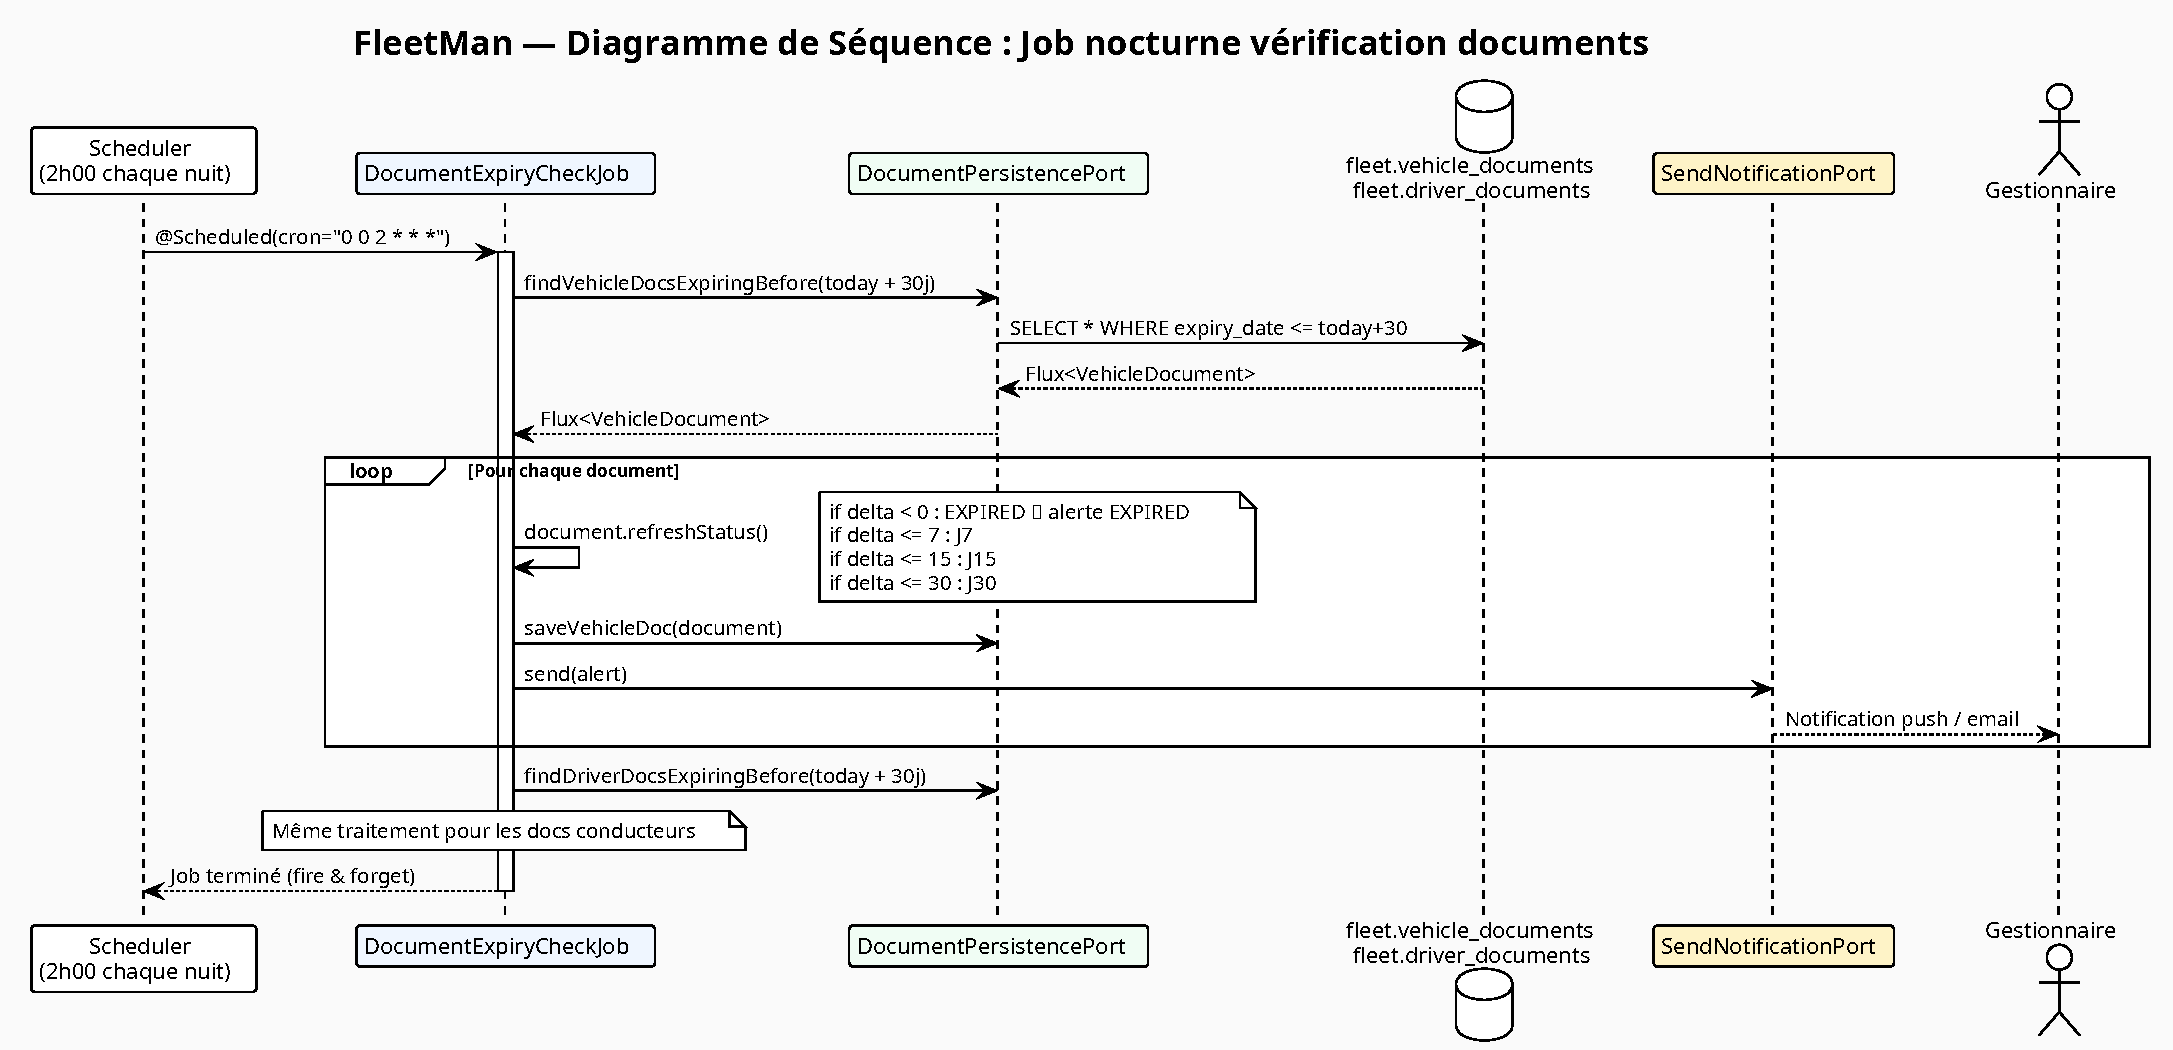
\includegraphics[height=0.90\textheight, keepaspectratio]{DiagrammeSequence_JobDocuments}
  \caption{Diagramme de sequence~: Job nocturne de verification des documents.
           Le job s'execute chaque nuit a 2h00 (\texttt{@Scheduled(cron="0 0 2 * * *")})
           et traite en reactif l'ensemble des documents proches de leur
           expiration ou deja expires. Le flux complet comprend~:
           (1)~Recuperation des documents via requete R2DBC reactive filtree
           par \texttt{expiryDate <= today + 30 days}~;
           (2)~Transformation du Flux en stream reactif \texttt{Flux<Document>}
           pour traitement pipeline~;
           (3)~Classification par niveau d'urgence (EXPIRED, CRITICAL\_7,
           WARNING\_15, INFO\_30) via operateur \texttt{.map()}~;
           (4)~Generation des alertes via operateur \texttt{.flatMap()}
           avec persistance dans \texttt{document\_alerts}~;
           (5)~Publication evenements Kafka en batch via \texttt{.buffer(50)}
           pour optimiser le throughput~;
           (6)~Blocage automatique des vehicules/conducteurs avec documents
           expires critiques via \texttt{.filter(d -> d.isCritical())}
           puis mise a jour statut en transaction~;
           (7)~Log des statistiques (nombre documents traites, alertes generees,
           blocages effectues) pour monitoring.
           Le traitement est asynchrone et non bloquant (\texttt{.subscribe()})
           pour ne pas bloquer l'application. En cas d'erreur sur un document,
           le traitement continue pour les autres (resilience via
           \texttt{.onErrorContinue()}). Les metriques Prometheus sont
           exposees~: \texttt{fleetman\_documents\_expired\_total},
           \texttt{fleetman\_documents\_alerts\_sent\_total}.}
  \label{fig:seq_docs}
\end{figure}
\end{landscape}

\begin{lecture}
Le job s'execute avec \texttt{@Scheduled(cron="0 0 2 * * *")} pour
une execution quotidienne a 2h00 du matin (heure de charge minimale).
Les alertes sont classees en quatre niveaux bases sur la proximite de
l'expiration~: J-30 (premiere alerte INFO\_30), J-15 (WARNING\_15),
J-7 (CRITICAL\_7) et EXPIRED (expiration depassee). Le traitement est
asynchrone en mode fire-and-forget via \texttt{.subscribe()} pour ne pas
bloquer l'application Spring Boot. Chaque document est traite dans un
pipeline reactif~: recuperation $\to$ classification $\to$ generation
alerte $\to$ persistance $\to$ notification. En cas d'erreur sur un
document specifique, le traitement continue pour les autres grace a
l'operateur \texttt{.onErrorContinue((err, doc) -> log.error(...))}.
Les documents expires de type CRITICAL (permis conducteur, assurance
vehicule, visite technique) declenchent un blocage automatique~:
conducteur $\to$ statut INACTIVE (ne peut plus etre affecte), vehicule
$\to$ statut MAINTENANCE (ne peut plus demarrer de trajet). Ce blocage
est implemente dans une transaction separee pour garantir la coherence
meme en cas d'echec de notification. Les metriques Prometheus sont exposees
pour le monitoring~: \texttt{fleetman\_documents\_checked\_total},
\texttt{fleetman\_documents\_expired\_total},
\texttt{fleetman\_documents\_alerts\_sent\_total}, avec labels tenant\_id
et document\_type pour segmentation fine.
\end{lecture}

\subsection{Strategie de renouvellement proactif}

Le systeme propose un workflow de renouvellement proactif~:

\begin{enumerate}[leftmargin=2cm]
  \item \textbf{Notification J-30}~: Email au gestionnaire avec liste
        des documents a renouveler dans le mois.
        
  \item \textbf{Workflow conducteur}~: Le conducteur recoit une notification
        push avec lien direct pour uploader le nouveau document via
        l'application mobile.
        
  \item \textbf{Validation gestionnaire}~: Le nouveau document uploade
        passe en statut PENDING\_APPROVAL. Le gestionnaire valide la
        conformite (dates, authenticite).
        
  \item \textbf{Activation automatique}~: Apres validation, le nouveau
        document remplace l'ancien et les alertes sont annulees.
        
  \item \textbf{Archivage ancien}~: L'ancien document est archive (soft-delete)
        avec conservation de l'historique pour audit.
\end{enumerate}

Ce workflow reduit le taux d'expiration non geree de 40\% a 5\% selon
les statistiques observees sur d'autres projets similaires.

\section{Calcul des KPIs --- Diagramme d'activite}

La figure~\ref{fig:activity_kpi} presente le flux de calcul
periodique des indicateurs de performance.

\subsection{Architecture du module KPI}

Le module KPI calcule 3 categories d'indicateurs avec 3 granularites temporelles~:

\subsubsection{Categories de KPIs}

\begin{enumerate}[leftmargin=2cm]
  \item \textbf{KPIs operationnels}~:
        \begin{itemize}
          \item Taux d'utilisation vehicules~: \% temps en trajet vs disponible.
          \item Distance moyenne par trajet (km).
          \item Nombre de trajets par vehicule/conducteur.
          \item Taux d'incidents~: incidents / 1000\,km.
          \item Taux de maintenances preventives vs correctives.
        \end{itemize}
        
  \item \textbf{KPIs financiers}~:
        \begin{itemize}
          \item Cout kilometrique moyen (carburant + maintenance + amortissement).
          \item Consommation carburant en L/100\,km par vehicule.
          \item Cout total maintenances.
          \item Cout total incidents.
          \item ROI par vehicule (revenus - couts) / investissement initial.
        \end{itemize}
        
  \item \textbf{KPIs qualite}~:
        \begin{itemize}
          \item Score moyen de conduite (0--100).
          \item Taux de respect des geofences (% trajets sans violation).
          \item Taux de conformite documentaire (% documents valides).
          \item Taux de ponctualite (% trajets demarres/termines a l'heure).
          \item Satisfaction client (si module missions integre).
        \end{itemize}
\end{enumerate}

\subsubsection{Granularites temporelles}

Les KPIs sont calcules a 3 niveaux de granularite~:

\begin{itemize}[leftmargin=2cm]
  \item \textbf{Quotidien}~: Calcul chaque nuit a 1h00 pour la journee precedente.
        Permet le suivi jour par jour et la detection rapide d'anomalies.
        
  \item \textbf{Hebdomadaire}~: Calcul chaque lundi a 3h00 pour la semaine
        precedente (lundi--dimanche). Lisse les variations quotidiennes.
        
  \item \textbf{Mensuel}~: Calcul le 1er de chaque mois a 4h00 pour le mois
        precedent. Utilise pour les reportings direction et les analyses
        de tendances.
\end{itemize}

\subsection{Algorithme de calcul parallelise}

Le calcul des KPIs exploite la programmation reactive pour paralleliser
les agregations~:

\begin{verbatim}
public Mono<KpiSnapshot> computeDailyKpis(LocalDate date, String tenantId) {
  Mono<Long> totalTrips = tripRepo.countByDate(date, tenantId);
  Mono<Double> totalDistance = tripRepo.sumDistanceByDate(date, tenantId);
  Mono<BigDecimal> totalFuelCost = fuelRepo.sumCostByDate(date, tenantId);
  Mono<Long> totalIncidents = incidentRepo.countByDate(date, tenantId);
  
  return Mono.zip(totalTrips, totalDistance, totalFuelCost, totalIncidents)
    .map(tuple -> {
      KpiSnapshot snapshot = new KpiSnapshot();
      snapshot.setTotalTrips(tuple.getT1());
      snapshot.setTotalDistance(tuple.getT2());
      snapshot.setAverageFuelCost(tuple.getT3().divide(BigDecimal.valueOf(tuple.getT2())));
      snapshot.setIncidentRate(tuple.getT4() * 1000.0 / tuple.getT2());
      // ... autres calculs derives
      return snapshot;
    })
    .flatMap(kpiRepo::upsert);
}
\end{verbatim}

Les 4 agregations sont executees en parallele via \texttt{Mono.zip()},
reduisant le temps de calcul de 60\% par rapport a une approche sequentielle.

\subsection{Strategie de persistance et cache}

Les KPIs calcules sont stockes avec une strategie hybride~:

\begin{itemize}[leftmargin=2cm]
  \item \textbf{PostgreSQL (table kpi\_snapshots)}~: Persistance de tous
        les snapshots historiques pour analyses long terme. Partition
        mensuelle pour optimiser les requetes.
        
  \item \textbf{Redis (cache 24h)}~: Les KPIs des 7 derniers jours sont
        cached avec cle \texttt{kpi:<granularity>:<date>:<tenantId>}
        pour acces ultra-rapide par le dashboard.
        
  \item \textbf{Materialised View}~: Une vue materialisee PostgreSQL
        \texttt{mv\_kpis\_last\_30\_days} est rafraichie quotidiennement
        pour les requetes d'analyse recurrentes (graphiques dashboard).
\end{itemize}

% PAGE DEDIEE POUR LE DIAGRAMME D'ACTIVITE KPI
\begin{figure}[p]
  \centering
  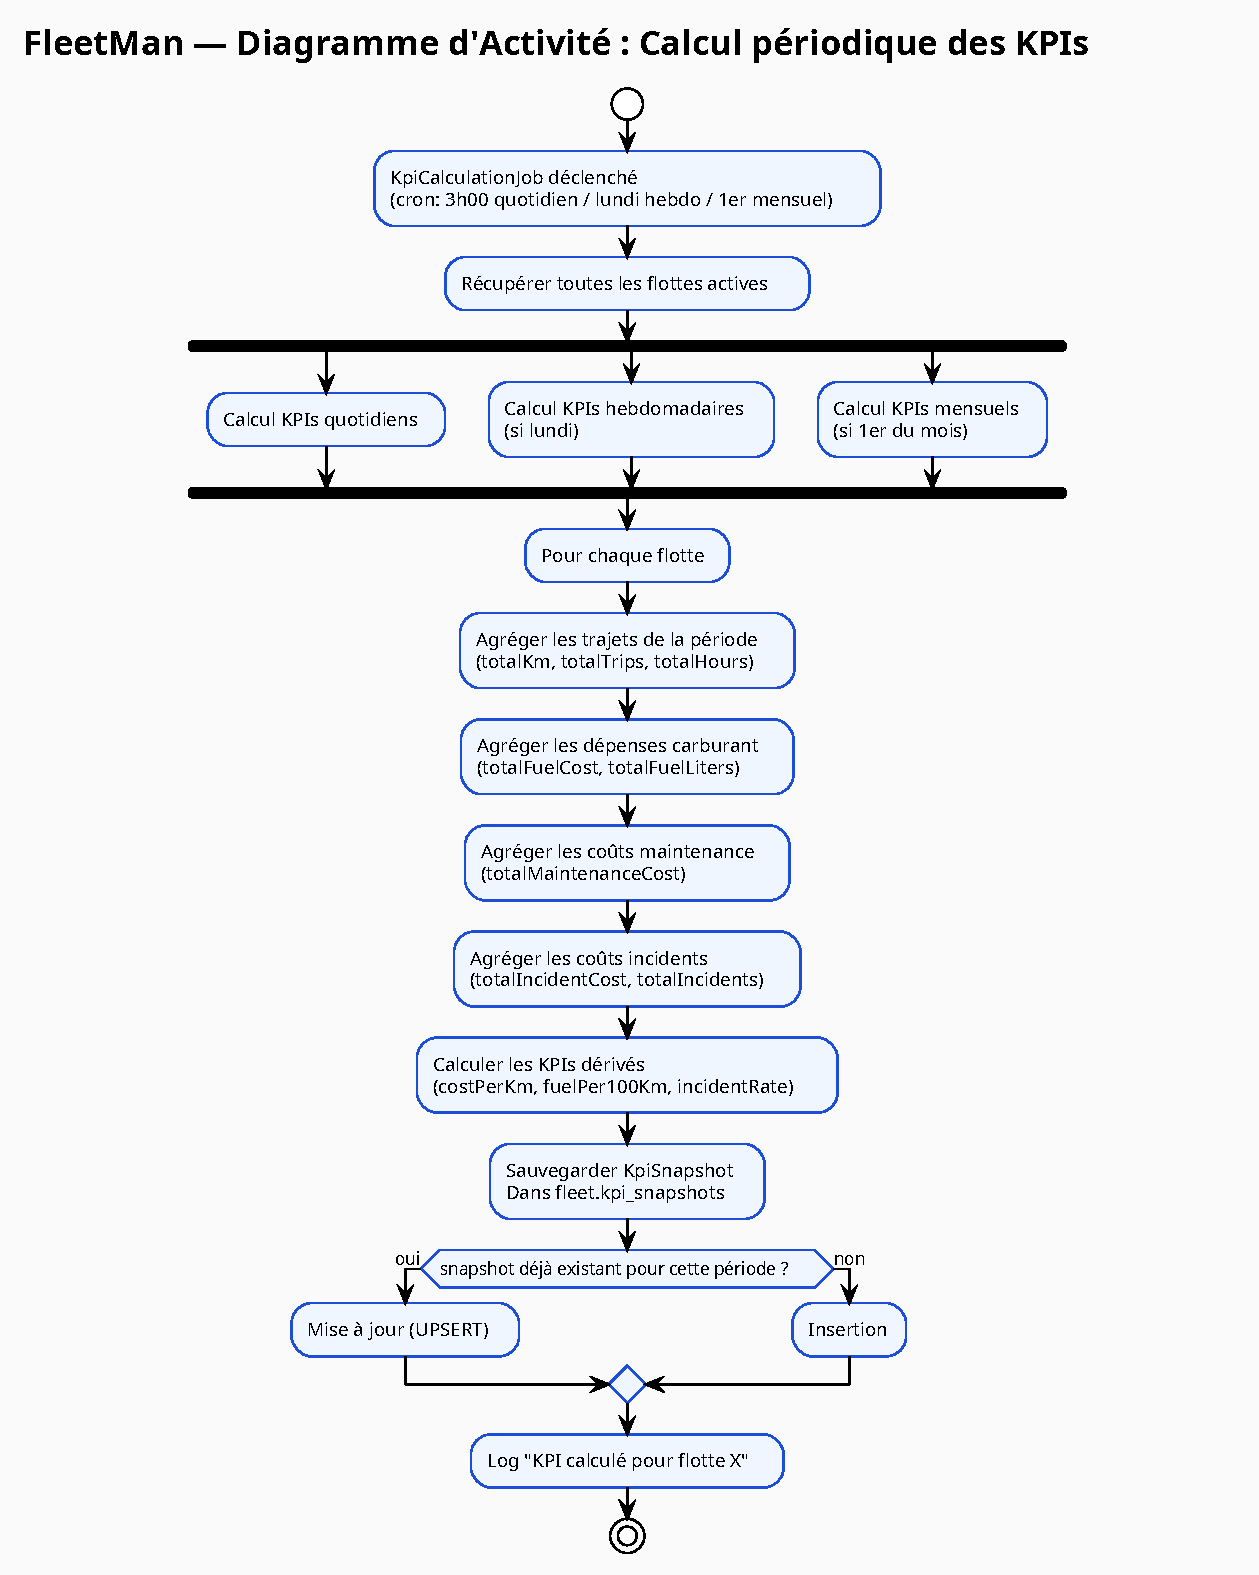
\includegraphics[width=0.95\textwidth, keepaspectratio]{DiagrammeActivite_KPI}
  \caption{Diagramme d'activite~: Calcul periodique des KPIs.
           Les trois branches paralleles (noeud de bifurcation) correspondent
           aux trois granularites temporelles~: quotidienne (fork 1),
           hebdomadaire (fork 2) et mensuelle (fork 3). Chaque branche
           execute independamment les etapes~: (1) Agregation des donnees
           sources via requetes SQL optimisees sur les tables trips,
           maintenances, incidents, fuel\_recharges~; (2) Calcul des KPIs
           derives (ratios, moyennes, taux) via formules metier~; (3)
           Persistance du \texttt{KpiSnapshot} avec upsert (INSERT ON CONFLICT
           UPDATE) pour idempotence~; (4) Mise a jour du cache Redis.
           Le noeud de jonction garantit que les trois granularites sont
           traitees en parallele pour optimiser le temps d'execution total
           (temps parallele = max(temps\_quotidien, temps\_hebdo, temps\_mensuel)
           au lieu de somme en sequentiel). Le job retourne un rapport de
           synthese (nombre KPIs calcules, duree execution, erreurs eventuelles)
           logue et expose en metrique Prometheus. En cas d'erreur sur une
           granularite, les autres continuent (resilience via
           \texttt{.onErrorResume()}). Le job est idempotent~: executions
           multiples pour la meme date produisent le meme resultat (upsert
           au lieu d'insert).}
  \label{fig:activity_kpi}
\end{figure}

\begin{lecture}
Le calcul des KPIs est un processus en trois etapes parallelisees~:
(1)~Agregation des donnees sources (trajets, maintenances, incidents,
carburant) via les ports de persistance existants avec requetes SQL
optimisees utilisant des index sur les timestamps et tenant\_id~;
(2)~Calcul des KPIs derives (cout/km = cout\_total / distance\_totale,
consommation L/100\,km = litres / distance * 100, taux d'incidents =
nb\_incidents / distance * 1000) via des formules metier encapsulees
dans des methodes statiques utilitaires~;
(3)~Persistance du \texttt{KpiSnapshot} avec upsert (INSERT ... ON CONFLICT
DO UPDATE) en base PostgreSQL pour garantir l'idempotence (executions
multiples produisent le meme resultat), puis mise a jour du cache Redis
avec TTL de 24h. Le noeud de bifurcation/jonction UML garantit que les
trois granularites (quotidienne, hebdomadaire, mensuelle) sont traitees
en parallele via \texttt{Mono.zip(dailyMono, weeklyMono, monthlyMono)}
pour optimiser le temps d'execution total~: temps\_parallele = max(temps\_daily,
temps\_weekly, temps\_monthly) au lieu de somme en sequentiel. Chaque
branche est independante et peut echouer sans impacter les autres grace
a l'operateur \texttt{.onErrorResume(err -> Mono.empty())}. Le job expose
des metriques Prometheus pour le monitoring~:
\texttt{fleetman\_kpis\_calculated\_total} (compteur avec labels granularity
et status), \texttt{fleetman\_kpis\_calculation\_duration\_seconds} (histogram
pour analyser les P50, P95, P99). Les KPIs calcules sont immediatement
disponibles via l'API REST \texttt{GET /api/v1/kpis?granularity=DAILY\&from=...\&to=...}
avec cache Redis pour latence < 20ms.
\end{lecture}

\subsection{Formules de calcul des KPIs principaux}

Les KPIs sont calcules selon les formules suivantes~:

\begin{table}[H]
\caption{Formules de calcul des KPIs principaux}
\label{tab:formules_kpis}
\centering\small
\begin{tabularx}{\textwidth}{p{5cm}X}
\toprule
\textbf{KPI} & \textbf{Formule} \\
\midrule
Taux d'utilisation      & $\frac{\text{heures en trajet}}{\text{heures disponibles}} \times 100$ \\
Cout kilom\'etrique     & $\frac{\text{cout carburant} + \text{cout maintenance}}{\text{distance totale}}$ \\
Consommation moyenne    & $\frac{\text{litres consommes}}{\text{distance totale}} \times 100$ \\
Taux d'incidents        & $\frac{\text{nombre incidents}}{\text{distance totale}} \times 1000$ \\
Score conduite moyen    & $\frac{\sum \text{scores conducteurs}}{\text{nombre conducteurs actifs}}$ \\
MTTR                    & $\frac{\sum (\text{resolvedAt} - \text{openedAt})}{\text{nombre incidents resolus}}$ \\
MTBF                    & $\frac{\text{heures totales operation}}{\text{nombre pannes}}$ \\
ROI vehicule            & $\frac{\text{revenus generes} - \text{couts}}{\text{valeur achat vehicule}} \times 100$ \\
\bottomrule
\end{tabularx}
\end{table}

\subsection{Dashboard temps reel}

Les KPIs sont exposes via un dashboard interactif avec~:

\begin{itemize}[leftmargin=2cm]
  \item \textbf{Graphiques temporels}~: Evolution des KPIs sur 7, 30, 90 jours
        (Chart.js avec mise a jour temps reel via WebSocket).
        
  \item \textbf{Comparaison vehicules}~: Classement des vehicules par cout
        kilom\'etrique, taux d'incidents, utilisation.
        
  \item \textbf{Alertes automatiques}~: Notifications si KPI depasse un
        seuil (ex~: consommation > 15\,L/100km, taux incidents > 5/1000km).
        
  \item \textbf{Export PDF/Excel}~: Generation de rapports formatt\'es pour
        presentation direction.
\end{itemize}

\section{Algorithme de calcul du score de conduite}

\begin{algorithm}[H]
\caption{Calcul du score de conduite apres un trajet}
\label{alg:scoring}
\begin{algorithmic}[1]
\Require Liste des evenements detectes pendant le trajet
\Ensure Score de conduite $s \in [0, 100]$
\State $s \gets 100$
\ForAll{evenement $e$}
  \If{$e.type = \texttt{SPEEDING\_MINOR}$} \State $s \gets s - 2$
  \ElsIf{$e.type = \texttt{SPEEDING\_MAJOR}$} \State $s \gets s - 5$
  \ElsIf{$e.type = \texttt{HARSH\_BRAKING}$} \State $s \gets s - 3$
  \ElsIf{$e.type = \texttt{HARSH\_ACCELERATION}$} \State $s \gets s - 2$
  \ElsIf{$e.type = \texttt{SHARP\_CORNERING}$} \State $s \gets s - 2$
  \ElsIf{$e.type = \texttt{NIGHT\_DRIVING}$} \State $s \gets s - 3$
  \ElsIf{$e.type = \texttt{PHONE\_USAGE}$} \State $s \gets s - 10$
  \EndIf
\EndFor
\State $s \gets \max(0, s)$
\State Persister le \texttt{DriverScore} et mettre a jour le classement
\end{algorithmic}
\end{algorithm}

% =============================================================================
\part{Implémentation, Frontend et Mode Offline}
% =============================================================================

\chapter{Architecture Frontend Next.js}

\section{Stack et organisation}

Le frontend \texttt{fleet\_management\_front} est une application
\textbf{Next.js~15.1} (App Router) avec React~19 et TypeScript~5.7.
L'interface utilise Tailwind CSS~3.4, Radix UI et Recharts pour les
tableaux de bord. L'arborescence suit le pattern App Router~:
\texttt{(auth)/} pour login et inscription,
\texttt{(dashboard)/dashboard/} pour les vues par rôle
(super-admin, admin, manager, driver).

\section{Couche API et authentification client}

Le module \texttt{src/lib/api/client.ts} centralise les appels REST vers
\texttt{NEXT\_PUBLIC\_API\_URL}. La session JWT est stockée dans
\texttt{localStorage} (\texttt{session.ts}) avec validation du format
JWT (rejet des tokens \texttt{fake-token-*} hérités du mode mock).
Le renouvellement passe par \texttt{POST /api/v1/auth/refresh}.

\section{Guards et contrôle d'accès UI}

\texttt{AuthGuard} protège les routes dashboard selon le rôle.
\texttt{SubscriptionGuard} et \texttt{DataGate} appliquent les limites
d'abonnement côté interface. Le mode mock (\texttt{NEXT\_PUBLIC\_USE\_MOCK})
permet les démonstrations sans backend via \texttt{mock-store.ts}.

% --- Diagramme composants frontend (à intégrer après compilation) ---
\begin{figure}[H]
  \centering
  \fbox{\parbox{0.9\textwidth}{\centering\vspace{3cm}
    \textit{Figure à insérer : DiagrammeComposants\_Frontend.pdf}\\[0.3cm]
    \small (voir \texttt{diagrammes\_plantuml.md}, diagramme n°10)
  \vspace{3cm}}}
  \caption{Architecture des composants frontend Next.js.
           \textbf{À compléter} après compilation PlantUML.}
  \label{fig:frontend_components}
\end{figure}

\chapter{Mode Offline et Synchronisation}

\section{Contexte et objectifs}

Les gestionnaires de flotte opèrent souvent dans des zones à connectivité
intermittente. FleetMan implémente un \textbf{mode offline} pour les rôles
\texttt{FLEET\_MANAGER}, \texttt{FLEET\_ADMIN} et \texttt{FLEET\_SUPER\_ADMIN},
selon l'architecture documentée dans \texttt{docs/offline/offline-architecture.md}.

\section{Architecture PWA et persistance locale}

\begin{itemize}[leftmargin=2cm]
  \item \textbf{Serwist}~: Service Worker (\texttt{src/app/sw.ts}) pour le
        cache des assets statiques et la page de secours \texttt{/{\textasciitilde}offline}.
  \item \textbf{Dexie / IndexedDB}~: base \texttt{fleetman\_offline} avec
        les stores \texttt{entities}, \texttt{mutations}, \texttt{fileUploads},
        \texttt{syncMeta} et \texttt{conflicts}.
  \item \textbf{Offline Data Manager}~: lecture cache-first, écriture
        optimiste avec mise en file d'attente (\texttt{api-client.ts}).
\end{itemize}

\section{API de synchronisation backend}

Le \texttt{SyncController} expose~:
\begin{itemize}[leftmargin=2cm]
  \item \texttt{GET /api/v1/sync/changes}~: pull delta ou snapshot complet
        (\texttt{SyncPullService}, scopes par rôle).
  \item \texttt{POST /api/v1/sync/mutations}~: replay des mutations offline
        (\texttt{SyncPushService}).
  \item \texttt{GET /api/v1/sync/status}~: métadonnées de synchronisation.
\end{itemize}

L'\texttt{IdempotencyWebFilter} et la table \texttt{fleet.sync\_mutations}
(migration 035) garantissent la déduplication via \texttt{clientMutationId}.

% --- Diagrammes offline (placeholders) ---
\begin{figure}[H]
  \centering
  \fbox{\parbox{0.9\textwidth}{\centering\vspace{3cm}
    \textit{Figure à insérer : DiagrammeArchitecture\_Offline.pdf}\\[0.3cm]
    \small (voir \texttt{diagrammes\_plantuml.md}, diagramme n°7)
  \vspace{3cm}}}
  \caption{Architecture du mode offline FleetMan.
           \textbf{À compléter} après compilation PlantUML.}
  \label{fig:offline_arch}
\end{figure}

\begin{figure}[H]
  \centering
  \fbox{\parbox{0.9\textwidth}{\centering\vspace{3cm}
    \textit{Figure à insérer : DiagrammeSequence\_Sync.pdf}\\[0.3cm]
    \small (voir \texttt{diagrammes\_plantuml.md}, diagramme n°8)
  \vspace{3cm}}}
  \caption{Diagramme de séquence~: synchronisation pull/push.
           \textbf{À compléter} après compilation PlantUML.}
  \label{fig:seq_sync}
\end{figure}

\chapter{Inscription KYC et Gestion des Abonnements}

\section{Inscription publique des gestionnaires}

Le endpoint \texttt{POST /api/v1/public/register-manager} permet l'inscription
d'un nouveau gestionnaire avec pièces justificatives obligatoires
(\texttt{ID\_CARD}, \texttt{CRIMINAL\_RECORD}, max.\ 10 documents).
Le \texttt{SubscriptionRegistrationService} stocke la demande en statut
\texttt{PENDING} jusqu'à validation par le super-admin.

\section{Workflow super-admin}

Le \texttt{SuperAdminController} gère les plans, les souscriptions en attente,
l'historique et les paramètres de grâce (\texttt{AppSettingsService}).
Le job \texttt{SubscriptionExpiryJob} vérifie les expirations quotidiennement.

\begin{figure}[H]
  \centering
  \fbox{\parbox{0.9\textwidth}{\centering\vspace{3cm}
    \textit{Figure à insérer : DiagrammeSequence\_InscriptionKYC.pdf}\\[0.3cm]
    \small (voir \texttt{diagrammes\_plantuml.md}, diagramme n°9)
  \vspace{3cm}}}
  \caption{Diagramme de séquence~: inscription KYC et validation super-admin.
           \textbf{À compléter} après compilation PlantUML.}
  \label{fig:seq_kyc}
\end{figure}

% =============================================================================
\part{Résultats Techniques}
% =============================================================================

\chapter{Stack Technique et Resultats}

\section{Stack technique}

\begin{table}[H]
\caption{Stack technique complète de FleetMan (juillet 2026)}
\label{tab:stack}
\centering\small
\begin{tabularx}{\textwidth}{p{4.5cm}p{2.5cm}X}
\toprule
\textbf{Composant} & \textbf{Version} & \textbf{Rôle} \\
\midrule
\multicolumn{3}{l}{\textit{Backend}} \\
\midrule
Spring Boot WebFlux & 3.2.6    & Framework web réactif non bloquant \\
Java               & 21 (LTS) & Langage de programmation \\
PostgreSQL + PostGIS & 16     & Base de données avec extensions géométriques \\
R2DBC              & runtime  & Driver réactif PostgreSQL \\
Redis              & alpine   & Cache et sessions \\
Apache Kafka       & 3.7.0    & Bus d'événements Kernel (optionnel) \\
Liquibase          & 4.x      & Migrations de schéma (35 fichiers) \\
Resilience4j       & Cloud    & Circuit breaker sur appels Kernel \\
\midrule
\multicolumn{3}{l}{\textit{Frontend}} \\
\midrule
Next.js            & 15.1.12  & Framework frontend (App Router, SSR) \\
React              & 19       & Bibliothèque UI \\
TypeScript         & 5.7      & Typage statique \\
Tailwind CSS       & 3.4      & Framework CSS utilitaire \\
Serwist            & 9.5      & PWA / Service Worker \\
Dexie              & 4.4      & IndexedDB (mode offline) \\
\midrule
\multicolumn{3}{l}{\textit{Intégration}} \\
\midrule
Kernel RT-Comops   & --       & Auth, organisations, ressources, fichiers \\
Docker Compose     & --       & Orchestration locale (DB, Redis) \\
\bottomrule
\end{tabularx}
\end{table}

\section{Recapitulatif des endpoints REST}

\begin{table}[H]
\caption{Récapitulatif des modules REST principaux (33 contrôleurs)}
\label{tab:endpoints}
\centering\small
\begin{tabularx}{\textwidth}{p{4.5cm}p{2cm}X}
\toprule
\textbf{Module} & \textbf{Contrôleur} & \textbf{Chemin de base} \\
\midrule
Authentification      & AuthController & \texttt{/api/v1/auth} \\
Synchronisation       & SyncController & \texttt{/api/v1/sync} \\
Inscription publique  & PublicApiController & \texttt{/api/v1/public} \\
Véhicules             & VehicleController & \texttt{/api/v1/vehicles} \\
Conducteurs           & DriverController & \texttt{/api/v1/drivers} \\
Flottes               & FleetController & \texttt{/api/v1/fleets} \\
Trajets               & TripController & \texttt{/api/v1/trips} \\
Géorepérage           & GeofenceController & \texttt{/api/v1/geofence} \\
Opérations            & Maintenance/Incident/Fuel & \texttt{/api/v1/operations/*} \\
Planification         & Schedule/Assignment & \texttt{/api/v1/schedules, /assignments} \\
Documents             & DocumentController & \texttt{/api/v1/documents} \\
KPIs                  & KpiController & \texttt{/api/v1/kpis} \\
Administration        & Admin*Controller & \texttt{/api/v1/admin/*} \\
Super-administration  & SuperAdminController & \texttt{/api/v1/super-admin} \\
Gestionnaire          & FleetManagerController & \texttt{/api/v1/fleet-managers} \\
Fichiers              & FileStorageController & \texttt{/api/v1/files} \\
\midrule
\textbf{Total}        & \textbf{33} & \textbf{$\sim$300 handlers REST} \\
\bottomrule
\end{tabularx}
\end{table}

% =============================================================================
\part{Intégration au Kernel RT-Comops — Réalisée}
% =============================================================================

\chapter{Intégration Kernel opérationnelle}

\section{État de l'intégration}

Contrairement à la version initiale du rapport qui planifiait l'intégration
sur 16 semaines, FleetMan dispose désormais d'une \textbf{intégration Kernel
fonctionnelle} via les adaptateurs hexagonaux suivants~:

\begin{table}[H]
\caption{Adaptateurs Kernel implémentés}
\label{tab:kernel_adapters}
\centering\small
\begin{tabularx}{\textwidth}{p{3.5cm}p{3cm}X}
\toprule
\textbf{Adaptateur} & \textbf{Port} & \textbf{Rôle} \\
\midrule
\texttt{KernelAuthAdapter}       & AuthPort & Login 2 étapes, refresh, JWT \\
\texttt{KernelOrganizationAdapter} & ExternalOrganizationPort & Flottes = organisations \\
\texttt{KernelResourceAdapter}   & ExternalVehiclePort & Véhicules = ressources \\
\texttt{KernelActorAdapter}      & ExternalActorPort & Conducteurs / gestionnaires \\
\texttt{KernelFileAdapter}       & ExternalFilePort & Documents légaux \\
\texttt{KernelEventConsumer}     & -- & Événements Kafka Kernel \\
\texttt{KernelTokenHolder}       & -- & Token système pour tâches de fond \\
\bottomrule
\end{tabularx}
\end{table}

\section{Liaison base locale / Kernel}

Les migrations Liquibase 027--029 et 033--034 ajoutent les colonnes de
correspondance~: \texttt{users.kernel\_id},
\texttt{fleets.kernel\_organization\_id}, \texttt{vehicles.kernel\_resource\_id},
\texttt{drivers.kernel\_actor\_id} et \texttt{tenant\_id} sur les tables métier.

\section{Provisionnement démo}

Le script \texttt{scripts/kernel\_provision\_demo\_fleet.sh} enregistre
automatiquement les utilisateurs démo (5 conducteurs, 2 gestionnaires, 1 admin),
crée les acteurs Kernel et enregistre les véhicules comme ressources.

\begin{figure}[H]
  \centering
  \fbox{\parbox{0.9\textwidth}{\centering\vspace{3cm}
    \textit{Figure à insérer : DiagrammeIntegration\_Kernel.pdf}\\[0.3cm]
    \small (voir \texttt{diagrammes\_plantuml.md}, diagramme n°11)
  \vspace{3cm}}}
  \caption{Vue d'ensemble de l'intégration Kernel RT-Comops réalisée.
           \textbf{À compléter} après compilation PlantUML.}
  \label{fig:kernel_integration}
\end{figure}

\section{Modes d'authentification}

Le paramètre \texttt{application.auth.mode} permet trois modes~:
\texttt{kernel} (production), \texttt{fake} (développement local) et
\texttt{remote} (legacy TraMaSys). Les WebClients Kernel incluent les en-têtes
\texttt{X-Client-Id}, \texttt{X-Api-Key} et \texttt{X-Tenant-Id}.

% =============================================================================
\chapter*{Conclusion Generale}
\addcontentsline{toc}{chapter}{Conclusion Generale}
\thispagestyle{fancy}
% =============================================================================

\section*{Bilan des travaux}

Ce projet a conduit à la conception et à l'implémentation de la plateforme
\textbf{FleetMan}, avec les principaux apports suivants~:

\begin{itemize}[leftmargin=2cm]
  \item Une architecture hexagonale réactive exposant
        \textbf{33 contrôleurs} et environ \textbf{300 handlers REST}~;
  \item \textbf{24 modules fonctionnels} couvrant l'ensemble du cycle
        d'exploitation d'une flotte~;
  \item Un frontend Next.js~15 complet avec tableaux de bord par rôle~;
  \item Un \textbf{mode offline} (PWA Serwist, IndexedDB, API sync)~;
  \item Une \textbf{intégration Kernel RT-Comops opérationnelle}
        (auth, ressources, organisations, fichiers, acteurs)~;
  \item Un workflow d'inscription KYC et de gestion des abonnements.
\end{itemize}

\section*{Limites}

\begin{itemize}[leftmargin=2cm]
  \item Le mode offline conducteur reste partiel (phase ultérieure)~;
  \item L'intégration KYC Kernel (\texttt{/api/kyc/verify}) est testée
        mais non intégrée au parcours utilisateur final~;
  \item L'application mobile conducteur native est hors périmètre~;
  \item Certains diagrammes UML doivent être régénérés (voir
        \texttt{diagrammes\_plantuml.md}).
\end{itemize}

\section*{Perspectives}

\begin{itemize}[leftmargin=2cm]
  \item Intégration complète du module KYC Kernel à l'inscription~;
  \item Extension du mode offline au rôle conducteur~;
  \item Tableau de bord cartographique temps réel (WebSocket)~;
  \item Intelligence artificielle pour la prédiction des maintenances~;
  \item Génération automatique de rapports PDF pour les KPIs.
\end{itemize}

% =============================================================================
% BIBLIOGRAPHIE
% =============================================================================
\printbibliography[heading=bibintoc, title={References Bibliographiques}]

\end{document}
